% NOTE(mrksr): KOMA says about 60-70 letters per line and about 30 lines
% per page are desireable. Pretty much all theses have more so we also stay a
% bit above with about 85 letters and 40 lines for 17x24 and DIV=14. That's not
% so far from the standard typearea of a4paper with about 95 letters and 40
% lines.
\documentclass[
    paper=17cm:24cm,
    % paper=18cm:25.5cm,
    % paper=19cm:27cm,
    % a4paper,
    DIV=14,
    11pt,
    twoside,
    parskip=half,
    headsepline,
    toc=bibnumbered,
    listof=leveldown,
    captions=tableheading,
    chapterprefix=on,
    numbers=noendperiod,
]{scrbook}

% Standalone
\usepackage{currfile}
\usepackage{xstring} % standalone path magic

% Math
\usepackage{amsmath}
\usepackage{amssymb}
\usepackage{mathtools}
\usepackage{xfrac}

% Style
\usepackage[hypertexnames=false, unicode, pdfusetitle]{hyperref}
\usepackage[headsepline]{scrlayer-scrpage}
\usepackage{xcolor}
\usepackage{graphicx}
\usepackage[nobreak]{mdframed}

% Layout
\usepackage[font=small, labelfont=bf, format=plain, indention=1em]{caption}
\usepackage[skip=3pt]{subcaption}
\usepackage[standard,hyperref]{ntheorem}
\usepackage{booktabs}
\usepackage{tabularx}
\usepackage{colortbl}
\usepackage{siunitx}

% Navigation
\usepackage{url}
\usepackage[capitalise, nameinlink, noabbrev]{cleveref}
\crefformat{equation}{(#2#1#3)}
\usepackage[style=alphabetic, backend=biber, url=false, maxcitenames=1]{biblatex}

% Misc
\usepackage{pdfpages}
\usepackage{blindtext}

% TUM color theme
% Base Colors Corporate Design
\definecolor{tumblue}{HTML}{0065BD}
\definecolor{tumgreen}{HTML}{A2AD00}
\definecolor{tumorange}{HTML}{E37222}
\definecolor{tumivory}{HTML}{DAD7CB}
\definecolor{tumred}{HTML}{E53418} % not in Styleguide
\definecolor{tumviolet}{HTML}{69085A} % not in Styleguide

% Derived Colors
% https://kuler.adobe.com/create/color-wheel/
% https://portal.mytum.de/corporatedesign/print/styleguide/
% Grays - TUM
\definecolor{tumgray0}{HTML}{000000}
\definecolor{tumgray1}{HTML}{58585A}
\definecolor{tumgray2}{HTML}{9C9D9F}
\definecolor{tumgray3}{HTML}{D9DADB}
\definecolor{tumgray4}{HTML}{FFFFFF}

% Blues - TUM
\definecolor{tumblue0}{HTML}{003359}
\definecolor{tumblue1}{HTML}{005293}
\definecolor{tumblue2}{HTML}{0073CF}
\definecolor{tumblue3}{HTML}{64A0C8}
\definecolor{tumblue4}{HTML}{98C6EA}

% Greens - Adobe
\definecolor{tumgreen0}{HTML}{EAF900}
\definecolor{tumgreen1}{HTML}{AEBA00}
\definecolor{tumgreen2}{HTML}{8A9300}
\definecolor{tumgreen3}{HTML}{525800}

% Reds - Adobe
\definecolor{tumred0}{HTML}{F23719}
\definecolor{tumred1}{HTML}{CB2E15}
\definecolor{tumred2}{HTML}{90210F}
\definecolor{tumred3}{HTML}{65170B}

% Oranges - Adobe
\definecolor{tumorange0}{HTML}{F07824}
\definecolor{tumorange1}{HTML}{C9651E}
\definecolor{tumorange2}{HTML}{8E4715}
\definecolor{tumorange3}{HTML}{63320F}


% Siemens color theme
% Primary
\definecolor{sPetrol}{RGB}{0,153,153}
\definecolor{sStoneDark}{RGB}{60,70,75}
\definecolor{sStoneLight}{RGB}{135,155,170}
\definecolor{sStone}{RGB}{190,205,215}
\definecolor{sSandDark}{RGB}{115,100,90}
\definecolor{sSandLight}{RGB}{170,170,150}
\definecolor{sSand}{RGB}{215,215,205}
\definecolor{sSnow}{RGB}{255,255,255}

% Accent
\definecolor{sTealDark}{RGB}{0,100,110}
\definecolor{sTealLight}{RGB}{65,170,170}
\definecolor{sBlueDark}{RGB}{0,95,135}
\definecolor{sBlueLight}{RGB}{80,190,215}
\definecolor{sGreenDark}{RGB}{100,125,45}
\definecolor{sGreenLight}{RGB}{170,180,20}
\definecolor{sYellowDark}{RGB}{235,120,10}
\definecolor{sYellowLight}{RGB}{255,185,0}
\definecolor{sRedDark}{RGB}{100,25,70}
\definecolor{sRedLight}{RGB}{175,35,95}


% Custom colors
\definecolor{hannah0}{HTML}{d89d1c}
\definecolor{hannah1}{HTML}{d8801c}
\definecolor{hannah2}{HTML}{d8511c}
\definecolor{hannah3}{HTML}{d8bf1c}
\definecolor{hannah4}{HTML}{d8511c}


% We use precompiled images and do not add tikz for speed of compilation.
\newcommand{\includestandalonewithpath}[2][]{%
    \includegraphics[#1]{#2}
}
\newcommand{\includestandalone}[2][]{%
    \includegraphics[#1]{#2}
}
\endofdump
% Fonts
\usepackage{fontspec}
\usepackage{unicode-math}
\usepackage{libertinus}
\usepackage{microtype}

% Language
\usepackage[utf8]{luainputenc}
\usepackage{csquotes}
\usepackage[english, ngerman, main=english]{babel}
\selectlanguage{english}

% Sets
\newcommand{\Ab}{\mathbb{A}}
\newcommand{\Bb}{\mathbb{B}}
\newcommand{\Cb}{\mathbb{C}}
\newcommand{\Db}{\mathbb{D}}
\newcommand{\Eb}{\mathbb{E}}
\newcommand{\Fb}{\mathbb{F}}
\newcommand{\Gb}{\mathbb{G}}
\newcommand{\Hb}{\mathbb{H}}
\newcommand{\Ib}{\mathbb{I}}
\newcommand{\Jb}{\mathbb{J}}
\newcommand{\Kb}{\mathbb{K}}
\newcommand{\Lb}{\mathbb{L}}
\newcommand{\Mb}{\mathbb{M}}
\newcommand{\Nb}{\mathbb{N}}
\newcommand{\Ob}{\mathbb{O}}
\newcommand{\Pb}{\mathbb{P}}
\newcommand{\Qb}{\mathbb{Q}}
\newcommand{\Rb}{\mathbb{R}}
\newcommand{\Sb}{\mathbb{S}}
\newcommand{\Tb}{\mathbb{T}}
\newcommand{\Ub}{\mathbb{U}}
\newcommand{\Vb}{\mathbb{V}}
\newcommand{\Wb}{\mathbb{W}}
\newcommand{\Xb}{\mathbb{X}}
\newcommand{\Yb}{\mathbb{Y}}
\newcommand{\Zb}{\mathbb{Z}}

\newcommand{\Ac}{\mathcal{A}}
\newcommand{\Bc}{\mathcal{B}}
\newcommand{\Cc}{\mathcal{C}}
\newcommand{\Dc}{\mathcal{D}}
\newcommand{\Ec}{\mathcal{E}}
\newcommand{\Fc}{\mathcal{F}}
\newcommand{\Gc}{\mathcal{G}}
\newcommand{\Hc}{\mathcal{H}}
\newcommand{\Ic}{\mathcal{I}}
\newcommand{\Jc}{\mathcal{J}}
\newcommand{\Kc}{\mathcal{K}}
\newcommand{\Lc}{\mathcal{L}}
\newcommand{\Mc}{\mathcal{M}}
\newcommand{\Nc}{\mathcal{N}}
\newcommand{\Oc}{\mathcal{O}}
\newcommand{\Pc}{\mathcal{P}}
\newcommand{\Qc}{\mathcal{Q}}
\newcommand{\Rc}{\mathcal{R}}
\newcommand{\Sc}{\mathcal{S}}
\newcommand{\Tc}{\mathcal{T}}
\newcommand{\Uc}{\mathcal{U}}
\newcommand{\Vc}{\mathcal{V}}
\newcommand{\Wc}{\mathcal{W}}
\newcommand{\Xc}{\mathcal{X}}
\newcommand{\Yc}{\mathcal{Y}}
\newcommand{\Zc}{\mathcal{Z}}

% Random Variables
\newcommand{\rv}[1]{\symbf{#1}}
\newcommand{\map}[1]{#1^{\text{MAP}}}
% Matrix
\newcommand{\mat}[1]{\symbf{#1}}
\newcommand{\inv}{^{\raisebox{.2ex}{$\scriptscriptstyle-\mkern-1.5mu1$}}}
\newcommand{\tran}{^{\mkern-1.5mu\raisebox{.2ex}{$\scriptscriptstyle\mathsf{T}$}}}
\newcommand{\itran}{^{\raisebox{.2ex}{$\scriptscriptstyle-\mkern-1.5mu\mathsf{T}$}}}
\newcommand{\Eye}{\mat{\mathrm{I}}}
% Pseudo Inputs
\newcommand{\ps}[1]{\bar{#1}}
\newcommand{\psmat}[1]{\ps{\mat{#1}}}

% Nicer empty set
\renewcommand{\emptyset}{\varnothing}

% Math operators
% General
\DeclareMathOperator{\id}{id}
\DeclareMathOperator*{\argmax}{argmax}
\DeclareMathOperator*{\argmin}{argmin}
\DeclareMathOperator*{\argsup}{argsup}
\DeclareMathOperator*{\arginf}{arginf}
\DeclareMathOperator{\atanTwo}{atan2}
\DeclareMathOperator{\sgn}{sgn}
\DeclareMathOperator{\diag}{diag}
\DeclareMathOperator{\tr}{tr}
\DeclareMathOperator*{\maximize}{maximize}
\DeclareMathOperator*{\minimize}{minimize}
\DeclareMathOperator{\subjectto}{subject\ to}
\DeclareMathOperator{\Oh}{\mathcal{O}}
\DeclareMathOperator{\softmax}{softmax}
\newcommand{\Powerset}[1]{2^{#1}}
\newcommand*{\diff}{\mathop{}\!\mathrm{d}}
\DeclarePairedDelimiter{\abs}{\vert}{\vert}
\DeclarePairedDelimiter{\norm}{\Vert}{\Vert}
\newcommand{\nth}[2][th]{#2^{\text{#1}}}

% Probabilities
\DeclareMathOperator{\E}{\mathbb{E}}
\DeclareMathOperator{\cov}{cov}
\DeclareMathOperator{\var}{var}
\DeclareMathOperator{\corr}{\varrho}
\DeclareMathOperator{\p}{p}
\DeclareMathOperator{\q}{q}
\DeclareMathOperator{\KLdiv}{KL}
\DeclareMathOperator{\K}{\mathcal{K}}
\DeclareMathOperator{\Q}{\mathcal{Q}}
\DeclareMathOperator{\Norm}{\mathcal{N}\mkern2mu}
\DeclareMathOperator{\Multi}{\mathcal{M}}
\DeclareMathOperator{\Ber}{\mathcal{B}}
\DeclareMathOperator{\Uni}{\mathbb{U}}
\DeclareMathOperator{\Ind}{\mathbb{I}}
\DeclareMathOperator{\GP}{\mathcal{GP}}
\DeclareMathOperator{\ProbSpace}{\mathcal{P}\mkern1mu}
\DeclareMathOperator{\indep}{\perp\mkern-9.5mu\perp}
\DeclareMathOperator{\nindep}{\centernot{\indep}}

\providecommand\given{}
\DeclarePairedDelimiterX{\Cond}[1]{(}{)}{
    \renewcommand\given{%
        \nonscript\mkern2mu
        \delimsize\vert
        \nonscript\mkern2mu
        \mathopen{}
        \allowbreak}
    #1
}

\makeatletter
\newcommand{\Fun}{\@ifstar\@sfun\@fun}
\newcommand{\@fun}[1]{#1\Cond}
\newcommand{\@sfun}[1]{#1\Cond*}
\makeatother

\newcommand{\Probs}[1]{\ProbSpace_{#1}}
% \newcommand{\Probs}{\Fun*{\ProbSpace}}
\newcommand{\Prob}{\p\Cond}
\newcommand{\aProb}{\tilde{\p}\Cond}
\newcommand{\hProb}{\hat{\p}\Cond}
\newcommand{\Variat}{\q\Cond}
\newcommand{\Gaussian}{\Norm\Cond}
\newcommand{\Multinomial}{\Multi\Cond}
\newcommand{\Uniform}{\Uni\Cond}
\newcommand{\Indicator}{\Ind\Cond}

\DeclarePairedDelimiterX{\KLdelim}[2]{(}{)}{%
    #1\mkern2mu\delimsize\|\mkern2mu#2%
}
\newcommand{\KL}{\KLdiv\KLdelim}

\DeclarePairedDelimiterXPP{\Moment}[2]{#1}{[}{]}{}{
\renewcommand\given{%
    \nonscript\mkern2mu
    \delimsize\vert
    \nonscript\mkern2mu
    \mathopen{}
    \allowbreak}
#2
}

\providecommand\with{}
\DeclarePairedDelimiterX{\Set}[1]{\{}{\}}{
    \renewcommand\with{%
        \nonscript\mkern2mu
        \delimsize\vert
        \nonscript\mkern2mu
        \mathopen{}
        \allowbreak}
    #1
}

\DeclarePairedDelimiterXPP{\pix}[1]{\begingroup\scriptscriptstyle}{(}{)}{\endgroup}{\mkern-1mu#1\mkern-1mu}

% NOTE(mrksr): See https://tex.stackexchange.com/a/112212/34265
\makeatletter
\DeclareRobustCommand{\rvdots}{%
    \vbox{
        \baselineskip4\p@\lineskiplimit\z@
        \kern-\p@
        \hbox{.}\hbox{.}\hbox{.}
    }}
\makeatother


% Show overfull boxes
% \overfullrule=5pt

\addbibresource{zotero_export.bib}

\title{A unifying Bayesian formulation of Reinforcement Learning}
\author{
    Markus Kaiser\\
    \href{mailto:markus.kaiser@siemens.com}{\texttt{markus.kaiser@siemens.com}}
}
\makeatletter
\chead{\@title}
\makeatother

\setkomafont{labelinglabel}{\bfseries}

\begin{document}

\frontmatter

\maketitle
\begin{titlepage}
    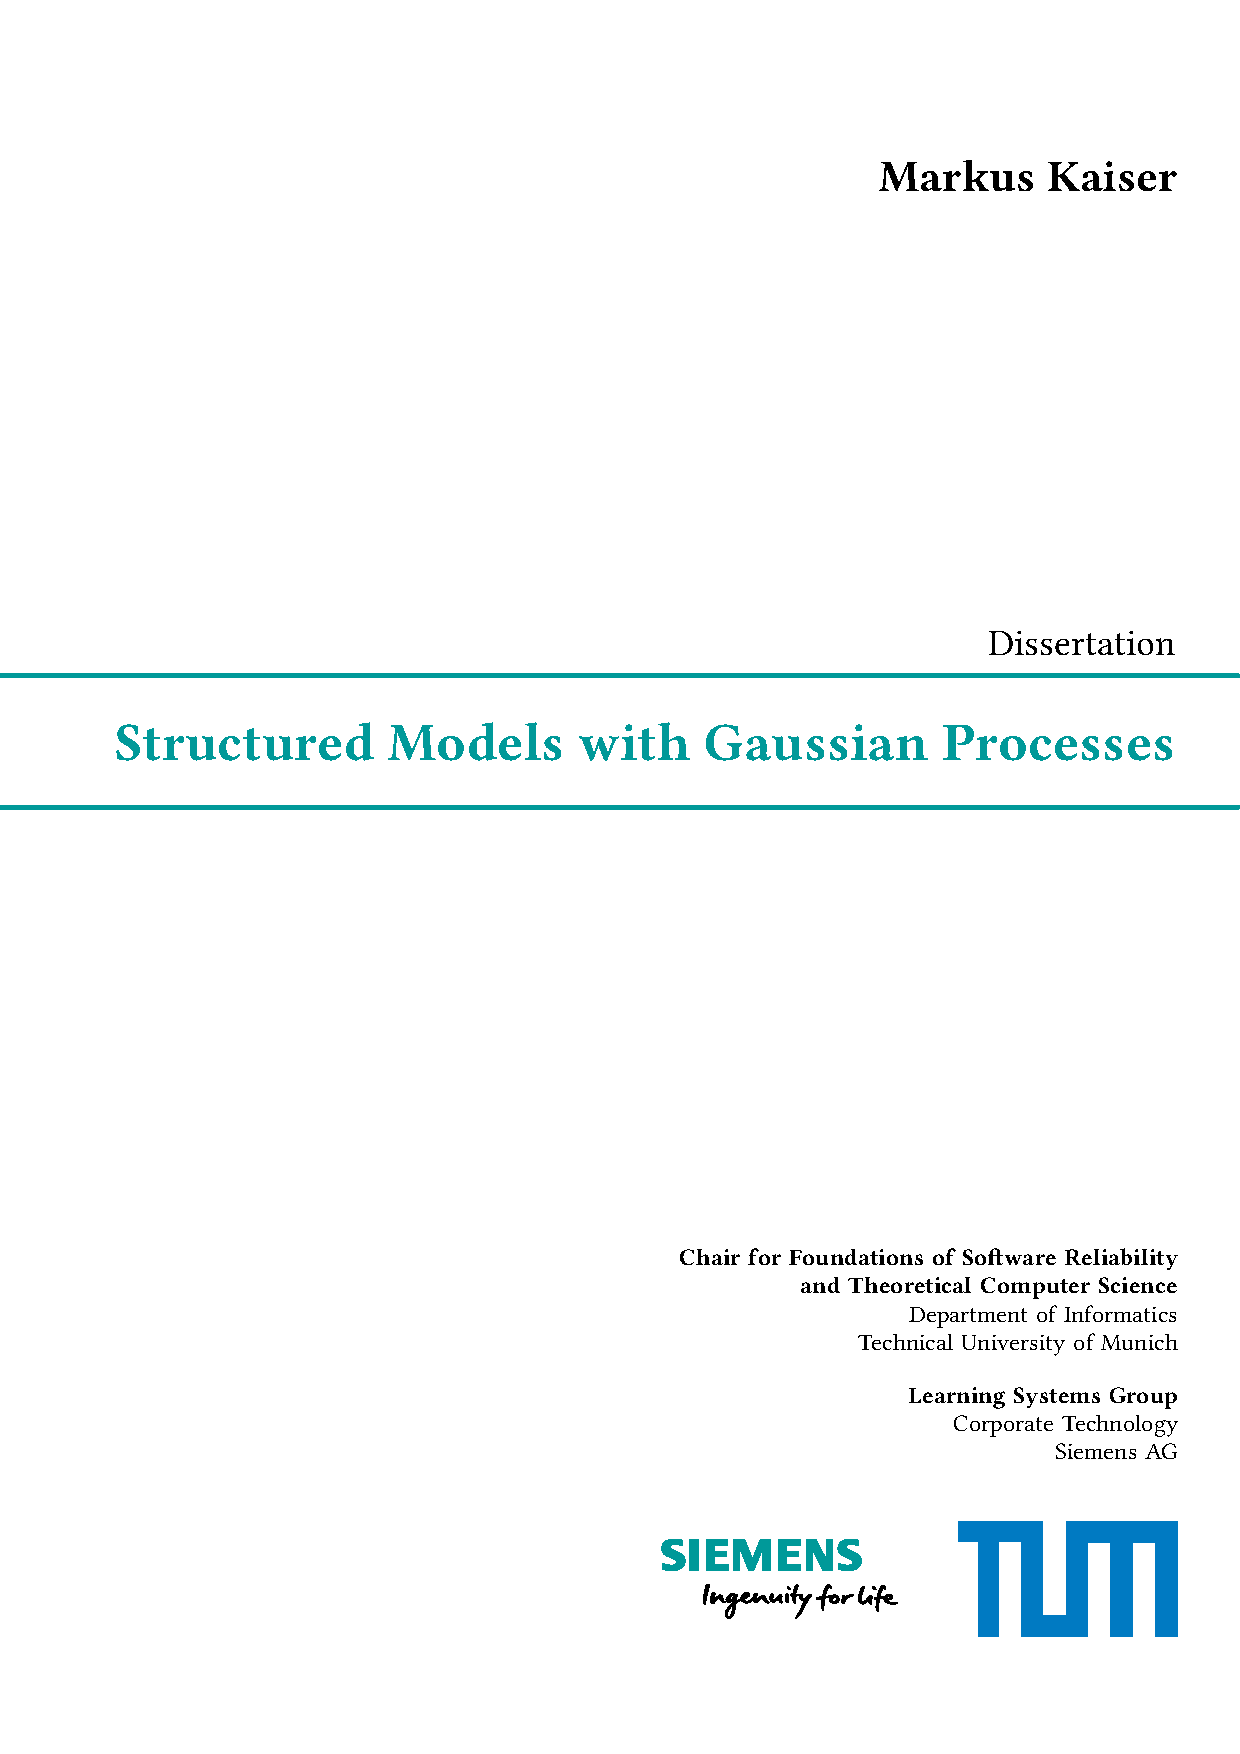
\includepdf{figures/title_page}
\end{titlepage}

\begin{titlepage}
    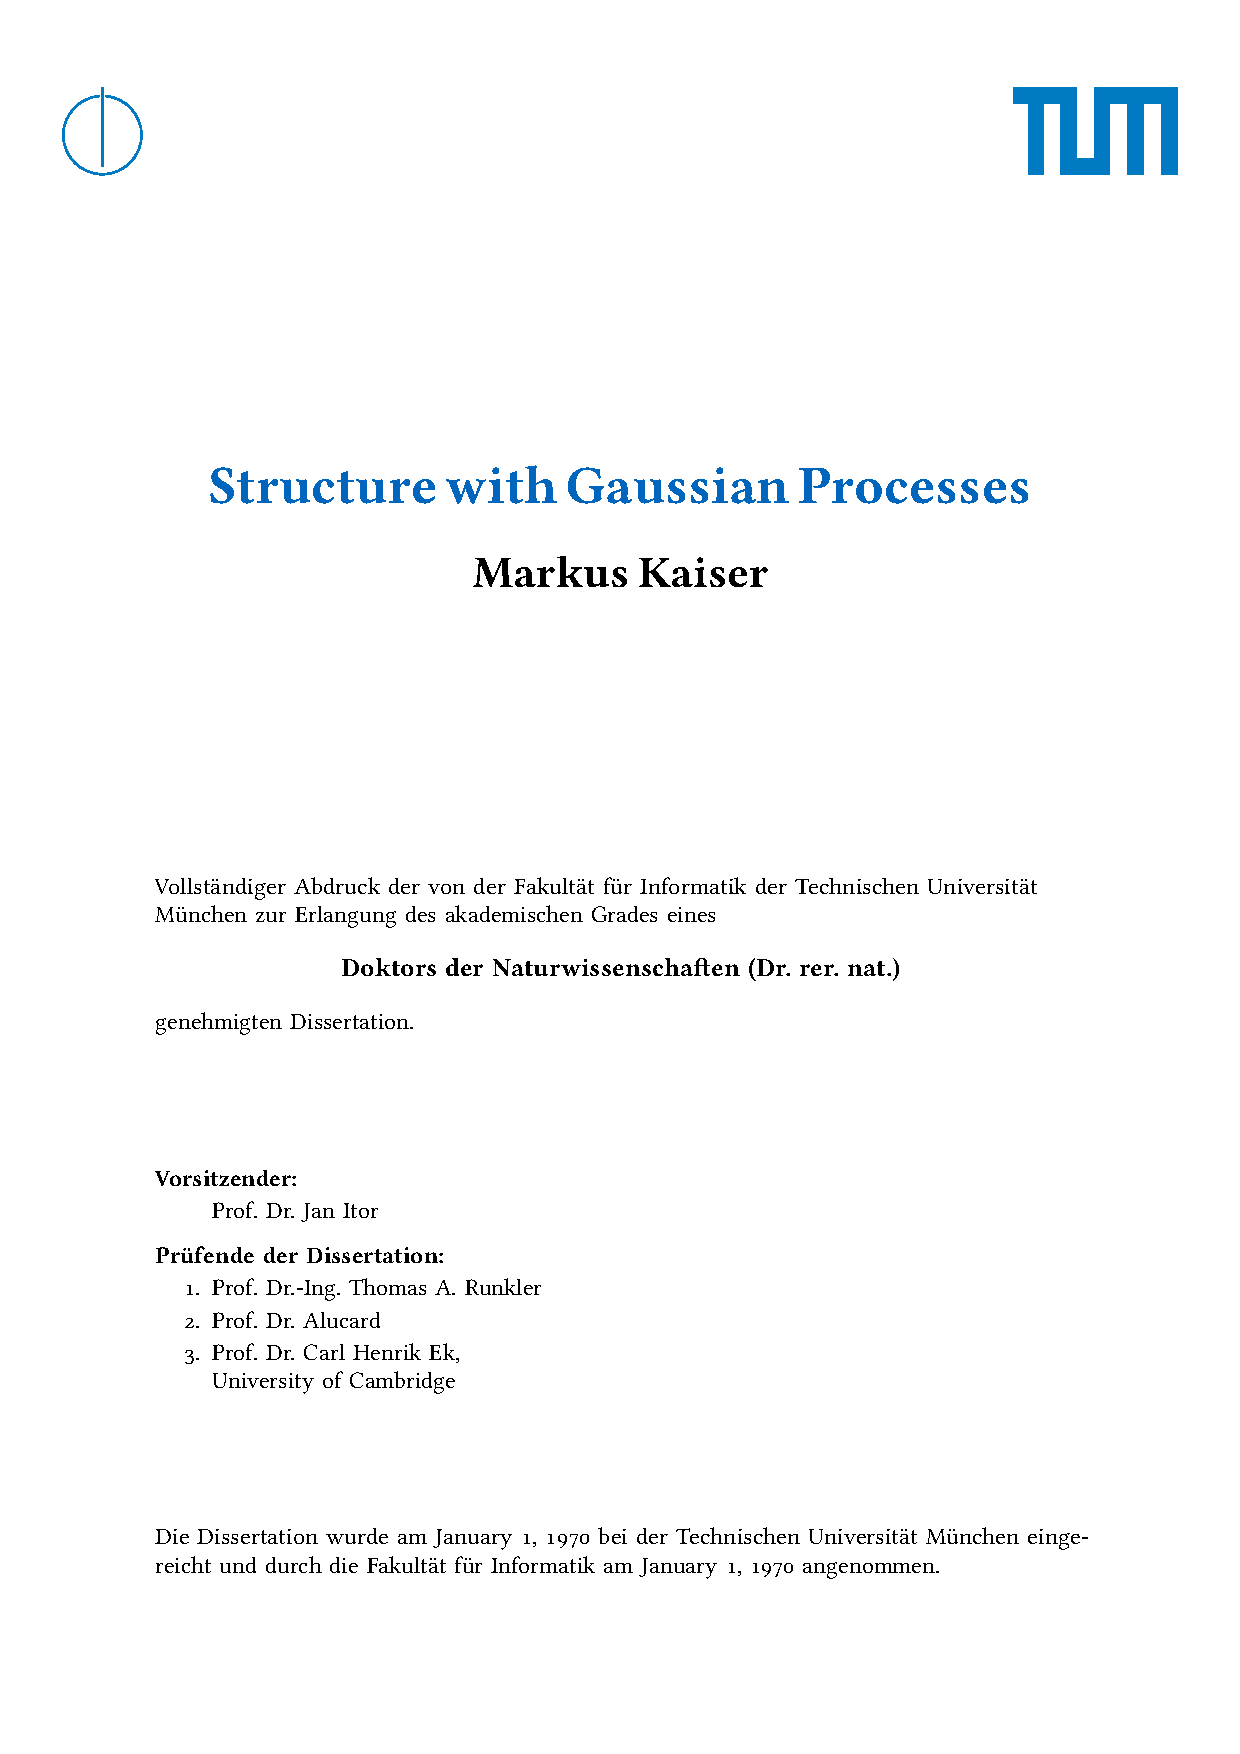
\includepdf{figures/title_page_tum}
\end{titlepage}

\begin{Abstract}{ngerman}
    \todoi{German abstract}
\end{Abstract}

\begin{Abstract}{english}
    Machine learning methods have seen great success recently in a wide range of digital domains such as speech recognition, computer vision or video games.
    However, bridging the gap to applications in the physical world has proved challenging as they introduce a new set of requirements.
    Machine learning systems must make efficient use of expert knowledge, handle low data regimes, and quantify uncertainties.
    This thesis studies how structured probabilistic models allow us to cope with these requirements.
    Structured models combine black-box and white-box modeling approaches to formalize expert knowledge while still being able to gain new insights from data.
    While in white-box models experts design components to describe a generative process in great detail, black-box models rely on general function approximators and trust that structure can be extracted given enough data.
    In structured models, we make use of available expert knowledge but accept that there are parts of the system we do not understand and model them using black-box components.
    Imposing structure allows us to characterize desired solutions and formulate what we want to learn from data.

    In this work, we study how to formulate Bayesian structural models using methods from Bayesian nonparametrics.
    We interpret recent advances in inference schemes for deep Gaussian processes in the context of structural models and formulate informative hierarchical priors.
    We discuss two approaches to adding structure based on mathematical formalization and expert-understanding of an underlying physical process.
    Using real-world industrial applications such as the detection of faulty sensors and the prediction of power generation in a wind-farm as examples, we show how structural priors lead to models with rich internal structure and physically plausible results.

    In situations where internal structure or generalization behavior come into focus, model selection using marginal likelihoods can be insufficient to identify desirable models.
    We consider how to formalize the subjectiveness in model selection through the task a model will be used to solve.
    We show that in a reinforcement learning problem, semantic models outperform other models with similar performance metrics and allow experts to influence agent behavior.
    We finally discuss why models with suboptimal marginal likelihoods can perform well in hierarchical systems and consider how to formulate Bayesian inference problems that take downstream tasks into account.
\end{Abstract}

\begin{Acknowledgements}
    I want to thank my supervisor Prof.~Dr.~Thomas A.~Runkler for his guidance and support.
    Thomas has always encouraged me to explore my ideas while offering invaluable advice and making sure I do not lose focus.
    I am very grateful to my co-supervisor Prof.~Dr.~Carl Henrik Ek for his enthusiasm and mentorship.
    He is an inspiring teacher and shows me what is important in academia.
    Thank you for welcoming me to your research group, making Bristol a second home for me, and the countless discussions about the big picture and the small details.
    I also want to thank my advisor Dr.~Clemens Otte for his valuable input and his exceptional ability to combine research and applications.
    I could not have asked for better supervision or a more encouraging research environment during my studies.

    I am thankful to everyone at Siemens and the Learning Systems group, especially Volkmar Sterzing for giving us PhD candidates the freedom to pursue our interests and enabling us to work on exciting industrial applications.
    I am grateful to Steffen Udluft and Hans Georg Zimmermann for always taking the time to discuss new ideas and for broadening my horizon as well as my fellow PhD candidates Stefan Depeweg, Daniel Hein and Phillip Swazinna for many discussions, whiteboard-drawings and meetings at the Biergarten.
    Thanks to Marion Eigner for her refreshing perspective and friendship.

    I feel lucky to be part of a motivating and unique group in Bristol and Bath.
    Thank you to Prof.~Dr.~Neill Campbell for your passion for good research and for your help in pursuing worthwhile ideas.
    I want to thank Erik Bodin, Ieva Kazlauskaite and Ivan Ustyuzhaniov for many thoughtful discussions and collaborations.

    A big thank you to my siblings Matthias and Andrea for your support and encouragement.
    I sincerely thank my parents, Pia and Robert Kaiser, for enabling and inspiring us to follow our dreams and for your unconditional support.
    Above all I want to thank Hannah for her patience and understanding while being in COVID-19 lockdown with a person writing their thesis.
    Thank you for all the lunches, the much-needed distractions, the happiness, and your love.
\end{Acknowledgements}

\listoftodos
\todototoc

\tableofcontents

\tableofcontents

\mainmatter
\chapter{Introduction}
\label{toc:introduction}
Everything is awesome, everything is cool when you're part of a team.
Everything is awesome, when you're living out a dream.

\chapter{Hierarchical Gaussian Processes}
\label{cha:hierarchical_gaussian_processes}

\section{Gaussian Processes}
\label{sec}
The transition dynamics $\Dyn \colon \Es \times \Ah \to \Dists(\Es^+)$ is a function mapping states and actions to a probability distribution of following states.
In order to estimate them using Gaussian processes, some assumptions about the structure of this function are needed.
First, it will be assumed that both the set of states $\Es$ and the set of actions $\Ah$ are euclidean real-valued vector spaces and that the set of terminal states $\Tee$ is empty, that is, $\Es^+$ and $\Es$ are assumed equal, requiring that episode endings have to be modelled separately.
And secondly, the probability distribution of the following state is assumed to be unimodal.
This unimodality can result from deterministic transition functions, such as the one of the bicycle benchmark defined in \cref{cha:the_bicycle_benchmark}, being disturbed slightly by Gaussian noise.

Estimating a function $f$ on the basis of observations $\mat{y_i} = f(\mat{x_i}) + \epsilon_i \in \R$ with input vectors $\mat{x_i} \in \R^d$ and a noise term $\epsilon_i$ is a \emph{regression problem}.
Since the number of observations is finite and the function $f$ lives in an infinite dimensional function space, the estimation of $f$ is uncertain and based on prior assumptions about its structure.

In classic control scenarios, these prior assumptions often follow from physical descriptions of the system to be modelled.
While the physics of driving a bicycle is understood quite well and can be described using differential equations, a controller for a specific bicycle depends on some parameters $\rv{\eta}$ such as the masses and measures detailed in \cref{tab:bicycle_constants}.
In this setting, solving the regression problem corresponds to finding a choice of parameters $\rv{\eta^\ast}$ which explain the observations of the true system best.

In a Bayesian context, instead of deciding on one specific vector of parameters, it might be more interesting to derive a distribution $\Prob{\rv{\eta^\ast}}$ of probable parameter values which then represents the uncertainty about their true value.
When making a prediction for a new input point $\mat{x_\ast}$, this uncertainty can be used to derive a predictive distribution $\Prob{y_\ast \given \mat{x_\ast}, \mat{\eta^\ast}}$, which propagates this uncertainty through the model to the prediction.

This approach represents uncertainty about the correct choice of parameters but assumes that the predefined structure of the function is correct, making it a \emph{parametric model}.
Such structure has the advantage of making it easier to find the best set of parameters, since the search space is relatively limited.
It does, however, limit the expressiveness of the model, which can lead to bad performance.
A physical description of the system might be too idealized and not account for all real-world factors, such as the assumptions of frictionless mechanics or limited turbulences in fluid mechanics.
Accounting for all possible effects can make the model very complicated.
This means that both the number of parameters becomes large and it may be hard to interpret the model in a physical sense.

\emph{Non-parametric models} are not based on insights about the concrete structure of the function to be modelled but rather only make assumptions about properties of the function itself, such as smoothness or differentiability.
Instead of modeling a distribution of parameter values, a Bayesian non-parametric model is concerned with finding a distribution $\Prob{f^\ast}$ of probable functions which represents the belief of the model about the function $f$ to be estimated.

\emph{Gaussian processes (GPs)} are a state-of-the-art framework for non-parametric regression.
They are a way of representing a probability distribution over functions in a way which is both computationally feasible and allows for Bayesian inference.
This section introduces Gaussian processes and describes how to encode a prior distribution over functions to represent preference in the space of all possible functions $f$.
Based on observed data, GPs can be used make predictions about the predictive distribution $\Prob{y_\ast \given \mat{x_\ast}, f^\ast}$ taking all functions in the distribution $\Prob{f^\ast}$ into account.
Since these predictions are not computationally cheap, an extension of Gaussian processes for large data sets, sparse Gaussian processes using pseudo-inputs \cite{snelson_sparse_2005}, is reviewed last.

\subsection{Definition}
Gaussian processes are a generalization of the Gaussian distribution to function spaces.
A multivariate Gaussian $\mat{x} \sim \Gaussian{\mat{\mu}, \mat{\Sigma}}$ describes a distribution over the finitely many elements in the vector $\mat{x}$ \cite{gauss_theoria_1809}.
Every such element $\rv{x_i}$ is normally distributed according to $\rv{x_i} \sim \Gaussian{\mu_i, \Sigma_{ii}}$ with a particular dependency structure between them.
For every pair $(\rv{x_i}, \rv{x_j})$, their covariance is given by $\Moment{\cov}{\rv{x_i}, \rv{x_j}} = \mat{\Sigma}_{ij}$.

Modeling functions in general requires an infinite number of random variables, one for every function value.
An infinite number of possibly dependent random variables mapping from the same probability space to the same value space is called a \emph{stochastic process} and is represented via a function.

\begin{definition}[Stochastic Process]
    \label{def:stochastic_process}
    Given a probability space $(\Omega, \mathcal{F}, P)$, an index set $T$ and a measurable space $Y$, a \emph{stochastic process $\rv{X}$} is a function
    \begin{align}
        \rv{X} \colon \left\{\begin{aligned}
            T \times \Omega &\to Y \\
            (t, \omega) &\mapsto \rv{X_t}(\omega)
        \end{aligned}\right.
    \end{align}
    mapping indices $t$ to $Y$-valued random-variables.
    For a fixed $\omega \in \Omega$, $\rv{X}(\cdot, \omega)$ is called a \emph{trajectory} of the process \cite{astrom_introduction_1971}.
\end{definition}

The index set of a stochastic process can be an arbitrary set.
It is often interpreted as a time index which can be both discrete and continuous.
A Gaussian process is a particular stochastic process.
\begin{definition}[Gaussian Process]
    \label{def:gaussian_process}
    A stochastic process $\rv{X}$ is called a \emph{Gaussian process} if for any finite subset $\tau \subseteq T$ of its index set, the random variables $\rv{X}_\tau$ have a joint Gaussian distribution \cite{astrom_introduction_1971}.
\end{definition}
When using a Gaussian process $\rv{X}$ to model a function $f \colon A \to B$, the index set $T$ is assumed to be $A$ and all random variables are $B$-valued.
The random variable $\rv{X_a}$ then models the function value $f(a)$ for all $a \in A$.
Sampling a trajectory from $\rv{X}$ corresponds to sampling one possible function $f^\ast$.

Similar to the finite case, the random variables have a dependency structure.
Instead of a mean vector $\mat{\mu}$ and a covariance matrix $\mat{\Sigma}$, a Gaussian process is completely determined by a \emph{mean function} $\mu_f(a) = \Moment{\E}{f(a)}$ and a \emph{covariance function}
\begin{align}
    \begin{split}
        \K(a, a^\prime) &\coloneqq \Moment{\E}{(f(a) - \mu_f(a))(f(a^\prime) - \mu_f(a^\prime))} \\
        &= \Moment{\cov}{f(a), f(a^\prime)} \\
        &= \Moment{\cov}{\rv{X_a}, \rv{X_{a^\prime}}}
    \end{split}
\end{align}
with $a, a^\prime \in A$.
The mean function encodes the point-wise mean over all trajectories which could be sampled from $\rv{X}$.
The covariance function is also called a \emph{kernel} and describes the interaction between different parts of the function.
A function which is distributed according to a Gaussian process is denoted as $f \sim \GP\Cond{\mu_f, \K}$.

For convenience it is often assumed that the prior mean function $\mu_f$ is constant zero.
This assumption is without loss of generality \cite{rasmussen_gaussian_2006} since otherwise, the observations $\left( \mat{X}, \mat{y} \right)$ can be transformed to $\mat{y^\prime} = \mat{y} - \mu(\mat{X})$.
The Gaussian process based on the observations $\left( \mat{X}, \mat{y^\prime} \right)$ then only models the differences to the mean function.
It is the covariance functions which encode the assumptions about the underlying function.

\subsection{Kernels}
Gaussian processes are collections of random variables, any finite subset of which have a joint multivariate Gaussian distribution.
For any pair $(\rv{X_i}, \mat{X_j})$ of these random variables, their covariance is given by the covariance function $\Moment{\cov}{\rv{X_i}, \rv{X_j}} = \K(i, j)$.
The pairwise covariances in a multivariate Gaussian $\Gaussian{\mat{\mu}, \mat{\Sigma}}$ are given by its \emph{covariance matrix} $\mat{\Sigma}$.
For any finite set of random variables, the matrix obtained by pairwise application of the covariance function is called the \emph{Gram matrix}.
\begin{definition}[Gram Matrix]
    Given a non-empty set $A$, a function $\K \colon A^2 \to \R$ and two sets $X = \Set*{x_i \in A \with i \in [n]}$ and $Y = \Set*{y_j \in A \with j \in [m]}$.
    The $n \times m$ matrix
    \begin{align}
        \K(X, Y) = \mat{K_{XY}} \coloneqq \bigg( \K(x_i, y_j) \bigg)_{\substack{i \in [n], \\ j \in [m]}}
    \end{align}
    is called the \emph{Gram matrix} of $\K$ with respect to $X$ and $Y$ \cite{scholkopf_learning_2002}.
    The notation $[n]$ describes the set $\Set{1, \dots, n}$ of integers.
\end{definition}
In order for the Gram matrix to be a valid covariance matrix $\mat{\Sigma}$ of a Gaussian distribution, it must be positive definite.
\emph{Kernels} are functions which fulfill the property that for every possible subset of random variables, or more generally every set of elements in their domain, their induced Gram matrix is positive definite.
\begin{definition}[Kernel]
    Given a non-empty set $A$, a function
    \begin{align}
        \K \colon A^2 \to \R
    \end{align}
    is called a \emph{(positive definite) kernel} or \emph{covariance function}, if for any finite subset $X \subseteq A$, the Gram matrix $\K(X, X)$ is positive definite \cite{scholkopf_learning_2002}.
\end{definition}
The kernel is crucial in encoding the assumptions about the function a Gaussian process should estimate.
It is a measure of \emph{similarity} of different points in the observed data and of new points to be predicted.
A natural assumption to make is to assume that the closer together in the domain two points lie, the more similar their function values will be.
Similarly, to predict a test point, training points close to it are probably more informative than those further away.

But closeness is not the only possible reason two points could be similar.
Assume a function to be modeled which is a possibly noisy sinusoidal wave with a known frequency.
Then, two points which are a multiple of wavelengths apart should also have similar function values.
A kernel which is not only dependent on the distance between two points but also their position in the input space is called \emph{non-stationary}.
A simple example of such a non-stationary kernel is the linear kernel.
\begin{definition}[Linear Kernel]
    For a finite dimensional euclidean vector space $\R^d$, the \emph{linear kernel} is defined as
    \begin{align}
        \K_{\text{linear}}(\mat{x}, \mat{y}) \coloneqq \mat{x}\tran \mat{y} = \left\langle \mat{x}, \mat{y}\right\rangle.
    \end{align}
\end{definition}
Consider a function $f \colon \R \to \R$ which is distributed according to a Gaussian process with the linear kernel $f \sim \GP\Cond{\mat{0}, \K_{\text{linear}}}$.
According to the definition of Gaussian processes, for any two input numbers $x$, $y \in \R$ their corresponding random variables $\rv{f_x}$ and $\rv{f_y}$ have a joint Gaussian distribution
\begin{align}
    \begin{pmatrix}
        \rv{f_x} \\ \rv{f_y}
    \end{pmatrix} \sim \Gaussian*{\mat{0}, \begin{bmatrix}
        \K(x, x) & \K(x, y) \\
        \K(y, x) & \K(y, y)
    \end{bmatrix}}
\end{align}
where $\K = \K_{\text{linear}}$.
Assuming that both $x$ and $y$ are not equal to zero, the correlation coefficient $\corr$ of these two variables is given by
\begin{align}
    \begin{split}
        \Moment{\corr}{\rv{f_x}, \rv{f_y}} &= \frac{\Moment{\cov}{\rv{f_x}, \rv{f_y}}}{\sqrt{\Moment{\var}{\rv{f_x}\vphantom{\rv{f_y}}}}\sqrt{\Moment{\var}{\rv{f_y}}}} \\
              &= \frac{\K(x, y)}{\sqrt{\K(x, x)} \sqrt{\K(y, y)}} = \frac{xy}{\sqrt{\vphantom{y^2}x^2}\sqrt{\vphantom{y^2}y^2}} \in \left\{ -1, 1 \right\}.
    \end{split}
\end{align}
A correlation coefficient of plus or minus one implies that the value of one of the random variables is a linear function of the other.
Any function drawn from this Gaussian process, such as the ones shown in \cref{fig:gp_samples:linear}, is therefore a linear function.
This observation generalizes to higher dimensions \cite{rasmussen_gaussian_2006}.
Gaussian process regression with a linear kernel is equivalent to Bayesian linear regression.
\begin{figure}[p]
    \begin{subfigure}[b]{\halffigurewidth}
        \centering
        \includestandalonewithpath{figures/gp_prior_linear}
        \caption{
            Linear
            \label{fig:gp_samples:linear}
        }
    \end{subfigure}
    \hfill
    \begin{subfigure}[b]{\halffigurewidth}
        \centering
        \includestandalonewithpath{figures/gp_prior_rbf}
        \caption{
            RBF with $\sigma_f = 1$ and $l=1$
            \label{fig:gp_samples:rbf_normal}
        }
    \end{subfigure}\\[4ex]
    \begin{subfigure}[b]{\halffigurewidth}
        \centering
        \includestandalonewithpath{figures/gp_prior_rbf_amplitude}
        \caption{
            RBF with $\sigma_f = \sqrt{2}$ and $l=1$
            \label{fig:gp_samples:rbf_noisy}
        }
    \end{subfigure}
    \hfill
    \begin{subfigure}[b]{\halffigurewidth}
        \centering
        \includestandalonewithpath{figures/gp_prior_rbf_lengthscale}
        \caption{
            RBF with $\sigma_f = 1$ and $l=\sfrac{1}{4}$
            \label{fig:gp_samples:rbf_lengthscale}
        }
    \end{subfigure}
    \caption[Samples from GP priors]{
        Since the mean function $\mu_f$ is assumed to be constant zero, the kernel specifies the prior assumptions about the function.
        A dashed sample function can be drawn by sampling a multivariate Gaussian with the kernel's Gram matrix using a grid of discrete sampling positions.
        While samples from the linear kernel are always hyperplanes, the RBF kernel describes arbitrary smooth functions.
        The hyperparameters $l$ and $\sigma_f$ of the kernel describe the assumed dynamic range in $x$ and $y$ directions respectively.
        \label{fig:gp_samples}
    }
\end{figure}

Because of its restrictiveness, the linear kernel is not very relevant for real-world applications of Gaussian processes.
As described above, the similarity of two data points $\mat{x}$ and $\mat{y}$ is often dependent on their relative position.
A kernel which is a function of $\mat{x} - \mat{y}$ is called \emph{stationary} and is invariant to translations in the input space.
The most important stationary kernel is the squared exponential kernel.
\begin{definition}[Squared Exponential Kernel]
    \label{def:rbf_kernel}
    For a finite dimensional euclidean vector space $\R^d$, the \emph{squared exponential kernel} (or \emph{RBF kernel}) is defined as
    \begin{align}
        \K_{\text{SE}}(\mat{x}, \mat{y}) \coloneqq \sigma_f^2 \cdot \exp\!\left( -\frac{1}{2} (\mat{x} - \mat{y})\tran \mat{\Lambda}^{-1} (\mat{x} - \mat{y}) \right).
    \end{align}
    The parameter $\sigma_f^2 \in \R_{>0}$ is called the \emph{signal variance} and $\mat{\Lambda} = \diag(l_1^2, \dots, l_d^2)$ is a diagonal matrix of the squared \emph{length scales} $l_i \in \R_{>0}$.
\end{definition}
The similarity of two data points approaches one when they are close together and for larger distances approaches zero with exponential drop off.
It can be shown that this kernel represents all infinitely differentiable functions \cite{rasmussen_gaussian_2006}.
Gaussian processes with this covariance function are universal function approximators.

The squared exponential kernel is dependent on multiple parameters which influence its behaviour.
In contrast to weight parameters in linear regression or constants in physical models, these parameters do not specify the estimated function but rather the prior belief about this function.
In order to separate the two, they are called \emph{hyperparameters}.
The vector of all hyperparameters in a model is called $\mat{\theta}$.

The hyperparameters of the RBF kernel describe the expected dynamic range of the function.
The signal variance $\sigma_f^2$ specifies the average distance of function values from the mean function.
The different length scale parameters $l_i$ roughly specify the distance of data points along their respective axis required for the function values to change considerably.
\Cref{fig:gp_samples} compares sample functions drawn from Gaussian processes with the linear kernel and squared exponential kernels with different hyperparameters.

These plots show continuous functions being drawn from their respective processes.
It is however only possible to evaluate the Gaussian process at finitely many points and then connect the resulting samples.
Drawing the function values of a finite amount of sample input points $\mat{X_\ast}$ from a Gaussian process prior is equivalent to drawing a sample from the Gaussian $\Gaussian{\mat{0}, \mat{K_\ast}}$ where $\mat{K_\ast}$ is a short hand notation for $\K(\mat{X_\ast}, \mat{X_\ast})$.

\subsection{Predictions and Posterior}
In order to use Gaussian processes for regression, it is necessary to combine observations with a Gaussian process prior $f \sim \GP\Cond{\mat{0}, \K}$ in order to obtain a predictive posterior.
The $N$ data points observed are denoted as $\D = \left( \mat{X}, \mat{y} \right)$ with $\mat{y} = f(\mat{X}) + \Gaussian{\mat{0}, \sigma_n^2 \Eye}$ and $\abs{\mat{y}} = N$.
The observed function values $\mat{y}$ are assumed to not be the true latent function values $\mat{f} = f(\mat{X})$ but rather have some additive Gaussian noise which is independent and identically distributed for all observations.
The variance of this noise $\sigma_n^2$ is a hyperparameter of the Gaussian process model.

Assuming further that given the latent function and the input points, the observations are conditionally independent, their likelihood is given by
\begin{align}
    \begin{split}
        \Prob{\mat{y} \given f, \mat{X}} = \Prob{\mat{y} \given \mat{f}} &= \prod_{i = 1}^N \Prob{y_i \given f_i} \\
        &= \prod_{i = 1}^N \Gaussian{y_i \given f_i, \sigma_n^2} = \Gaussian{\mat{y} \given \mat{f}, \sigma_n^2 \Eye}
    \end{split}
\end{align}
because of the assumed noise model.
Given some vector of hyperparameters $\mat{\theta}$, the definition of Gaussian processes yields a joint Gaussian distribution for the latent function values $\mat{f}$ given by
\begin{align}
    \Prob{\mat{f} \given \mat{X}, \mat{\theta}} = \Gaussian*{\mat{f} \given \mat{0}, \mat{K_N}}
\end{align}
where $\mat{K_N} = \K(\mat{X}, \mat{X})$ denotes the Gram matrix of the observed data.
Combining the two distributions according to the law of total probability yields the probability distribution of the outputs conditioned on the inputs and is given by
\begin{align}
    \begin{split}
        \label{eq:gp_marginal_likelihood}
        \Prob{\mat{y} \given \mat{X}, \mat{\theta}} &= \int \Prob{\mat{y} \given \mat{f}} \Prob{\mat{f} \given \mat{X}, \mat{\theta}} \diff \mat{f} \\
        &= \int \Gaussian{\mat{y} \given \mat{f}, \sigma_n^2 \Eye} \Gaussian*{\mat{f} \given \mat{0}, \mat{K_N}} \diff \mat{f} \\
        &= \Gaussian{\mat{y} \given \mat{0}, \mat{K_N} + \sigma_n^2 \Eye}.
    \end{split}
\end{align}
Note that this distribution is obtained by integrating over all possible latent function values $\mat{f}$ and thereby taking all possible function realizations into account.
This integration is called the \emph{marginalization} of $\mat{f}$.
The closed form solution of the integral is obtained using well-known results about Gaussian distributions which are for example detailed in \cite{petersen_matrix_2008}.

Now consider a set of test points $\mat{X_\ast}$ for which the predictive posterior should be obtained.
By definition, the latent function values $\mat{f}$ of the training set and the latent function values of the test set $\mat{f_\ast} = f(\mat{X_\ast})$ have the joint Gaussian distribution
\begin{align}
    \Prob*{\begin{pmatrix}
        \mat{f} \\
        \mat{f_\ast}
    \end{pmatrix} \given \mat{X}, \mat{X_\ast}, \mat{\theta}} &= \Gaussian*{\begin{pmatrix}
        \mat{f} \\
        \mat{f_\ast}
    \end{pmatrix} \given \mat{0}, \begin{bmatrix}
        \mat{K_N} & \mat{K_{N\ast}} \\
        \mat{K_{\ast N}} & \mat{K_{\ast}}
    \end{bmatrix}}.
\end{align}
Adding the noise model to this distribution leads to the joint Gaussian of training outputs $\mat{y}$ and test outputs $\mat{f_\ast}$ which is given by
\begin{align}
    \Prob*{\begin{pmatrix}
        \mat{y} \\
        \mat{f_\ast}
    \end{pmatrix} \given \mat{X}, \mat{X_\ast}, \mat{\theta}} &= \Gaussian*{\begin{pmatrix}
        \mat{y} \\
        \mat{f_\ast}
    \end{pmatrix} \given \mat{0}, \begin{bmatrix}
        \mat{K_N} + \sigma_n^2 \Eye & \mat{K_{N\ast}} \\
        \mat{K_{\ast N}} & \mat{K_{\ast}}
    \end{bmatrix}}.
\end{align}

In this distribution, the training outputs $\mat{y}$ are known.
The predictive posterior for the test outputs $\mat{f_\ast}$ can be obtained by applying the rules for marginalization of multivariate Gaussians \cite{petersen_matrix_2008}, yielding another Gaussian distribution $\Prob{\mat{f_\ast} \given \mat{X}, \mat{y}, \mat{X_\ast}}$.
\begin{lemma}[GP predictive posterior]
    \label{lem:gp_posterior}
    Given a latent function with a Gaussian process distribution $f \sim \GP(\mat{0}, \K)$ and $N$ training points $\mat{X}$ with noisy observations of the form $\mat{y} = f(\mat{X}) + \Gaussian{\mat{0}, \sigma_n^2 \Eye}$.
    The predictive posterior $\mat{f_\ast}$ of the test points $\mat{X_\ast}$ is then given by
    \begin{align}
        \begin{split}
            \Prob{\mat{f_\ast} \given \mat{X}, \mat{y}, \mat{X_\ast}} &= \Gaussian*{\mat{f_\ast} \given \mat{\mu_\ast}, \mat{\Sigma_\ast}} \text{, where} \\
            \mat{\mu_\ast} &= \mat{K_{\ast N}} \left( \mat{K_N} + \sigma_n^2 \Eye \right)^{-1} \mat{y} \\
            \mat{\Sigma_\ast} &= \mat{K_\ast} - \mat{K_{\ast N}} \left( \mat{K_N} + \sigma_n^2 \Eye \right)^{-1} \mat{K_{N\ast}}.
        \end{split}
    \end{align}
\end{lemma}
\begin{figure}[t]
    \begin{subfigure}[b]{\halffigurewidth}
        \centering
        \includestandalonewithpath{figures/gp_posterior_prior}
        \caption{GP Prior}
        \label{fig:gp_posterior:prior}
    \end{subfigure}
    \hfill
    \begin{subfigure}[b]{\halffigurewidth}
        \centering
        \includestandalonewithpath{figures/gp_posterior_posterior}
        \caption{GP Posterior}
        \label{fig:gp_posterior:posterior}
    \end{subfigure}
    \caption[GP posterior]{
        \Cref{fig:gp_posterior:prior} shows a GP prior with an RBF kernel.
        After observing the black data points, the mean function of the posterior GP in \cref{fig:gp_posterior:posterior} is no longer constant zero.
        The dashed function samples of the posterior GP interpolate the data but can be different in-between.
        The shaded area represents the point wise mean plus and minus two times the standard deviation.
        \label{fig:gp_posterior}
    }
\end{figure}

This predictive posterior makes it possible to evaluate the function approximation based on the input at arbitrary points in the input space.
Since any set of these points always has a joint Gaussian distribution, the predictive posterior defines a new Gaussian process, which is the posterior Gaussian process given the observations.
This posterior process $\GP(\mu_\text{post}, \K_\text{post})$ has new mean and covariance functions given by
\begin{align}
    \begin{split}
        \mu_\text{post}(\mat{a}) &= \K(\mat{a}, \mat{X}) \left(\mat{K_N} + \sigma_n^2 \Eye \right)^{-1} \mat{y} \\
        \K_\text{post}(\mat{a}, \mat{b}) &= \K(\mat{a}, \mat{b}) - \K(\mat{a}, \mat{X}) \left( \mat{K_N} + \sigma_n^2 \Eye \right)^{-1} \K(\mat{X}, \mat{b}).
    \end{split}
\end{align}
Note that the posterior mean function is not necessarily the constant zero function.
\Cref{fig:gp_posterior} shows samples from a pair of prior and posterior Gaussian processes.

Computing the inverse $\left(\mat{K_N} + \sigma_n^2 \Eye \right)^{-1}$ costs $\Oh(N^3)$ but can be done as a preprocessing step since it is independent of the test points.
Predicting the mean function value of a single test point is a weighted sum of $N$ basis functions $\mu_\ast = \mat{K_{\ast N}} \mat{\beta}$ where $\mat{\beta} = \left(\mat{K_N} + \sigma_n^2 \Eye \right)^{-1} \mat{y}$ which can be precomputed.
After this precomputation, predicting the mean of a single test point costs $\Oh(N)$.
To predict its variance, it is still necessary to perform a matrix multiplication which costs $\Oh(N^2)$.
Since all of these operations are dependent on the number of training points, evaluating Gaussian processes on large data sets can be computationally expensive.
Before introducing sparse approximations with better asymptotic complexity, the next section deals with choosing good values for the vector of hyperparameters $\mat{\theta}$.

\subsection{Choosing Hyperparameters}
In the previous section, the hyperparameters $\mat{\theta}$ were assumed to be known and constant, that is, the prior assumptions about the function to be estimated were fixed.
In this case, Gaussian processes do not have a training stage, since any test point can be predicted according to the predictive posterior.
Usually however, the correct choice of hyperparameters is not clear a priori.
A major advantage of Gaussian processes is the ability to select hyperparameters from training data directly instead of requiring a scheme such as cross validation.

In a fully Bayesian setup, the correct way to model uncertainty about hyperparameters is to assign them a prior $\Prob{\mat{\theta}}$ and marginalize it to derive the dependent distributions
\begin{align}
    \Prob{f} &= \int \Prob{f \given \mat{\theta}} \Prob{\mat{\theta}} \diff \mat{\theta} \\
    \Prob{\mat{y} \given \mat{X}} &= \int \Prob{\mat{y} \given \mat{X}, \mat{\theta}} \Prob{\mat{\theta}} \diff \mat{\theta}. \label{eq:theta_posterior_integration}
\end{align}
Updating the belief about the distribution of the hyperparameters then becomes part of the process of obtaining a posterior model.
A new distribution is obtained by combining the prior with the likelihood of the training data observed using Bayes' theorem:
\begin{align}
    \begin{split}
        \Prob{\mat{\theta} \given \mat{X}, \mat{y}} &= \frac{\Prob{\mat{y} \given \mat{X}, \mat{\theta}} \Prob{\mat{\theta}}}{\Prob{\mat{y} \given \mat{X}}} \\
        &= \frac{\Prob{\mat{y} \given \mat{X}, \mat{\theta}} \Prob{\mat{\theta}}}{\int \Prob{\mat{y} \given \mat{X}, \mat{\theta}} \Prob{\mat{\theta}} \diff \theta}
    \end{split}
\end{align}
The integration required in \cref{eq:theta_posterior_integration} is very hard in practice \cite{rasmussen_gaussian_2006}, since $\mat{y}$ is a complicated function of $\mat{\theta}$.
Instead, a common approximation is to use a \emph{maximum-a-postiori (MAP)} estimate of the correct hyperparameters.
This estimate is obtained by maximizing $\Prob{\mat{\theta} \given \mat{X}, \mat{y}}$ and does not require evaluation of the denominator since it is constant.

For many choices of priors $\Prob{\mat{\theta}}$ this is still a hard problem.
But assuming a flat prior which assigns almost equal probability to all choices of hyperparameters, it holds that
\begin{align}
    \begin{split}
        \Prob{\mat{\theta} \mid \mat{X}, \mat{y}} &\propto \Prob{\mat{y} \given \mat{X}, \mat{\theta}} \\
        &= \int \Prob{\mat{y} \given \mat{f}, \mat{\theta}} \Prob{\mat{f} \given \mat{X}, \mat{\theta}} \diff \mat{f},
    \end{split}
\end{align}
that is, the posterior distribution is proportional to the likelihood term and can be obtained using a maximum likelihood estimate on the \emph{marginal likelihood} after integrating out the function values $\mat{f}$.
Optimizing this term is called a \emph{type II maximum likelihood estimate (ML-II)}.

The marginal likelihood is an integral over a product of Gaussians obtained from the noise model and the distribution of function values according to the Gaussian process definition.
It is given by
\begin{align}
    \begin{split}
        \label{eq:gp_f_marginalization}
        \Prob{\mat{y} \mid \mat{X}, \mat{\theta}} &= \int \Prob{\mat{y} \given \mat{f}, \mat{\theta}} \Prob{\mat{f} \given \mat{\theta}} \diff \mat{f} \\
        &= \int \Gaussian{\mat{y} \given \mat{f}, \sigma_n^2 \Eye} \cdot \Gaussian{\mat{f} \given \mat{0}, \mat{K_N}} \diff \mat{f} \\
        &= \Gaussian{\mat{y} \given \mat{0}, \mat{K_N} + \sigma_n^2 \Eye}
    \end{split}
\end{align}
The solution of this integral is a Gaussian density function \cite{petersen_matrix_2008}.
For practical reasons, it is convenient to minimize the negative logarithm of the likelihood which is given by
\begin{align}
    \begin{split}
        \Ell(\mat{\theta}) &= -\log\Prob{\mat{y} \given \mat{X}, \mat{\theta}} \\
        &= \frac{1}{2} \mat{y}\tran \left( \mat{K_N} + \sigma_n^2 \Eye \right)^{-1} \mat{y} +
        \frac{1}{2} \log \abs{\mat{K_N} + \sigma_n^2 \Eye} +
        \frac{N}{2} \log(2\pi).
    \end{split}
\end{align}
The estimation of hyperparameters is the solution of the optimization problem
\begin{align}
    \mat{\theta}^\ast &\in \argmin_{\mat{\theta}} \Ell(\mat{\theta})
\end{align}
and is calculated using standard approaches to non-convex optimization such as scaled conjugate gradient (SCD) techniques, since finding the derivatives of $\Ell$ is comparatively easy \cite{rasmussen_gaussian_2006}.
The computational complexity of evaluating the likelihood term and its derivatives is dominated by the inversion of $\mat{K_N} + \sigma_n^2 \Eye$.

Since this optimization scheme does not choose parameters of the function approximation directly but rather changes a small number of broad and high-level assumptions about it, overfitting does not tend to be a problem for Gaussian processes in general \cite{snelson_flexible_2007}.
The sparse approximation of Gaussian processes presented in the next section chooses a small number of points in the input space to represent a large training set.
The positions of these input points can be interpreted as hyperparameters to the original Gaussian process and induce a kernel function with many hyperparameters, where overfitting can become relevant.


\section{Sparse Approximations using Inducing Inputs}
A major drawback of Gaussian processes in real-world applications is their high computational cost for large data sets.
Assume a data set $(\mat{X}, \mat{y})$ with $N$ training samples, then the operations on a posterior Gaussian process are usually dominated by the inversion of the kernel matrix $\mat{K_N}$ which takes $\Oh(N^3)$ time.
While this is only a preprocessing step, the cost of predicting the mean and variance of one test point remains $\Oh(N)$ and $\Oh(N^2)$ respectively.
Additionally, these operations have a space requirement of $\Oh(N^2)$.
The goal of sparse approximations of Gaussian processes is to find model representations which avoid the cubic complexities or at least restrict them to the training phase of finding hyperparameters.
This section introduces one type of approximation based on representing the complete data set through a smaller set of points.

The most simple approach to achieve this is to only use a small subset of $M \ll N$ \emph{inducing} points of the original training set and learn a normal Gaussian process.
This approach can work for data sets with a very high level of redundancy but does impose the problem of choosing an appropriate subset.
While choosing a random subset can be effective \cite{snelson_flexible_2007}, the optimal choice is dependent on the hyperparameters and both should therefore be chosen in a joint optimization scheme.
This is a combinatorical optimization problem which can be very hard to solve in practice since the function to be optimized is very non-smooth.

To overcome this problem, \emph{sparse pseudo input Gaussian processes (SPGP)} \cite{snelson_flexible_2007} lift the restriction of choosing inducing points from the training set and instead allow arbitrary positions in the input space.
The original data set is replaced by a \emph{pseudo data set} $(\ps{\mat{X}}, \ps{\mat{f}})$ of \emph{pseudo inputs} $\ps{\mat{X}}$ and \emph{pseudo targets} $\ps{\mat{f}} = f(\ps{\mat{X}})$ which are equal to the true latent values of the function function $f \sim \GP(\mat{0}, \K)$.
Since they are not true observations, they are assumed to be noise-free.

With known positions of the pseudo inputs and fixed hyperparameters $\mat{\theta}$, the predictive posterior of a Gaussian process based on this pseudo data set for test points $(\mat{X_\ast}, \mat{f_\ast})$ is given by
\begin{align}
    \Prob{\mat{f_\ast} \given \mat{X_\ast}, \ps{\mat{X}}, \ps{\mat{f}}, \mat{\theta}} &= \Gaussian{\mat{K_{\ast M}}\mat{K_M}^{-1} \ps{\mat{f}}, \mat{K_\ast} - \mat{K_{\ast M}} \mat{K_M}^{-1} \mat{K_{M \ast}}}
\end{align}
according to \cref{lem:gp_posterior} with the notation $\mat{K_M} = \K(\ps{\mat{X}}, \ps{\mat{X}})$ meaning the Gram matrix of the pseudo inputs compared to $\mat{K_N} = \K(\mat{X}, \mat{X})$, the Gram matrix of the original training data.

The true data set is independent given the latent function and can therefore be assumed independent given the pseudo data set which should be a good representation of it.
The likelihood of the original data under the Gaussian process trained on the pseudo data set is given by
\begin{align}
    \begin{split}
        \Prob{\mat{y} \given \mat{X}, \ps{\mat{X}}, \ps{\mat{f}}, \mat{\theta}} &= \prod_{i=1}^N \Prob{y_n \given \mat{x_n}, \ps{\mat{X}}, \ps{\mat{f}}, \mat{\theta}} \\
        &= \prod_{i=1}^N \Gaussian*{y_n \given \mat{K_{n M}}\mat{K_M}^{-1} \ps{\mat{f}}, \mat{K_n} - \mat{K_{n M}} \mat{K_M}^{-1} \mat{K_{M n}} + \sigma_n^2} \\
        &= \Gaussian*{\mat{y} \given \mat{K_{N M}}\mat{K_M}^{-1} \ps{\mat{f}}, \diag\left( \mat{K_N} - \mat{K_{N M}} \mat{K_M}^{-1} \mat{K_{M N}} \right) + \sigma_n^2 \Eye} \\
        &= \Gaussian*{\mat{y} \given \mat{K_{N M}}\mat{K_M}^{-1} \ps{\mat{f}}, \diag\left( \mat{K_N} - \mat{Q_N} \right) + \sigma_n^2 \Eye}
    \end{split}
\end{align}
with $\mat{Q_N} \coloneqq \mat{K_{N M}} \mat{K_M}^{-1} \mat{K_{M N}}$.
The additive term $\sigma_n^2$ comes from the noise model assumed about the observations $\mat{y}$ in the original data set.
Rather than using maximum likelihood on this term to learn the complete pseudo data set $(\ps{\mat{X}}, \ps{\mat{f}})$, the pseudo targets $\ps{\mat{f}}$ can be marginalized.
This can be combared to the marginalization of the latent function values $\mat{f}$ in the derivation of Gaussian processes in \cref{eq:gp_f_marginalization}.
Assuming the pseudo targets to be distributed very similarly to the real data, a reasonable prior for them is given by
\begin{align}
    \Prob{\ps{\mat{f}} \given \ps{\mat{X}}} = \Gaussian{\ps{\mat{f}} \given \mat{0}, \mat{K_M}}.
\end{align}

The marginalization is stated as the integral of a product of two Gaussian distributions which has a closed form solution and is given by
\begin{align}
    \begin{split}
        \Prob{\mat{y} \given \mat{X}, \ps{\mat{X}}, \mat{\theta}} &= \int \Prob{\mat{y} \given \mat{X}, \ps{\mat{X}}, \ps{\mat{f}}, \mat{\theta}} \Prob{\ps{\mat{f}} \given \ps{\mat{X}}} \diff \ps{\mat{f}} \\
        &= \int \Prob{\mat{y} \given \mat{X}, \ps{\mat{X}}, \ps{\mat{f}}, \mat{\theta}} \Gaussian{\ps{\mat{f}} \given \mat{0}, \mat{K_M}} \diff \ps{\mat{f}} \\
        &= \Gaussian*{\mat{y} \given \mat{0}, \mat{K_{NM}} \mat{K_M}^{-1} \mat{K_M} \left( \mat{K_{NM}} \mat{K_M}^{-1} \right)\tran + \diag\left( \mat{K_N} - \mat{Q_N} \right) + \sigma_n^2 \Eye} \\
        &= \Gaussian*{\vphantom{\left( \mat{K_M}^{-1} \right)\tran} \mat{y} \given \mat{0}, \mat{Q_N} + \diag\left( \mat{K_N} - \mat{Q_N} \right) + \sigma_n^2 \Eye}.
    \end{split}
\end{align}
This \emph{SPGP marginal likelihood} can be interpreted as the marginal likelihood of a Gaussian process given the original data set $(\mat{X}, \mat{y})$ in \cref{eq:gp_marginal_likelihood}.
In this Gaussian process, the original kernel $\K$ is replaced by the kernel $\K_{\text{SPGP}}$.
With $\Ind$ denoting the indicator function, it is defined as
\begin{align}
    \begin{split}
        \Q(\mat{a}, \mat{b}) &\coloneqq \mat{K_{aM}} \mat{K_M}^{-1} \mat{K_{Mb}} \\
        \K_{\text{SPGP}}(\mat{a}, \mat{b}) &\coloneqq \Q(\mat{a}, \mat{b}) + \Indicator{\mat{a} = \mat{b}} \left( \K(\mat{a}, \mat{b}) - \Q(\mat{a}, \mat{b}) \right).
    \end{split}
\end{align}
This kernel is equal to $\K$ when both arguments are identical and equal to $\Q$ everywhere else.
For well-chosen pseudo inputs, $\mat{Q_N}$ is a low-rank approximation of $\mat{K_N}$ \cite{snelson_flexible_2007}.
Because of this identity, an SPGP is a normal Gaussian process with an altered kernel function.
The pseudo inputs $\ps{\mat{X}}$ are hidden in the kernel matrix $\mat{K_M}$ and are additional hyperparameters to this kernel.
This observation directly yields the SPGP predictive posterior using \cref{lem:gp_posterior}.
\begin{lemma}[SPGP predictive posterior]
    \label{lem:spgp_posterior}
    Given a latent function with a sparse pseudo-input Gaussian process distribution $f \sim \GP(\mat{0}, \K_{\text{SPGP}})$, $N$ training points $\mat{X}$ with noisy observations of the form $\mat{y} = f(\mat{X}) + \Gaussian{\mat{0}, \sigma_n^2 \Eye}$ and $M$ positions of pseudo-inputs $\ps{\mat{X}}$.
    The predictive posterior $\mat{f_\ast}$ of the test points $\mat{X_\ast}$ is then given by
    \begin{align}
        \begin{split}
            \Prob{\mat{f_\ast} \given \mat{X_\ast}, \mat{X}, \mat{y}, \ps{\mat{X}}} &= \Gaussian*{\mat{f_\ast} \given \mat{\mu_\ast}, \mat{\Sigma_\ast}} \text{, where} \\
            \mat{\mu_\ast} &= \mat{Q_{\ast N}} \left( \mat{Q_N} + \diag(\mat{K_N} - \mat{Q_N}) + \sigma_n^2 \Eye \right)^{-1} \mat{y} \\
            \mat{\Sigma_\ast} &= \mat{K_\ast} - \mat{Q_{\ast N}} \left( \mat{Q_N} + \diag(\mat{K_N} - \mat{Q_N}) + \sigma_n^2 \Eye \right)^{-1} \mat{Q_{N \ast}}.
        \end{split}
    \end{align}
    and $\mat{Q_N} \coloneqq \mat{K_{N M}} \mat{K_M}^{-1} \mat{K_{M N}}$.
\end{lemma}
\begin{figure}[tp]
    \begin{subfigure}{\halffigurewidth}
        \centering
        \includestandalonewithpath{figures/spgp_full}
        \caption{Full GP
            \label{fig:spgp_example:gp}
        }
    \end{subfigure}
    \hfill
    \begin{subfigure}{\halffigurewidth}
        \centering
        \includestandalonewithpath{figures/spgp_sparse}
        \caption{
            SPGP
            \label{fig:spgp_example:spgp}
        }
    \end{subfigure}
    \caption[SPGP example]{
        The black crosses signify data sampled from a noisy sine function.
        \Cref{fig:spgp_example:gp} shows a full GP trained on the complete data.
        \Cref{fig:spgp_example:spgp} shows an SPGP with pseudo inputs located at the dart positions.
        Since the pseudo function values are marginalized, only their $x$-coordinate is meaningful.
        Three pseudo inputs are enough to approximate the full GP with reasonable accuracy.
        \label{fig:spgp_example}
    }
\end{figure}

The predictive distribution as written in the previous equations can easily be compared to the predictive posterior of Gaussian processes in \cref{lem:gp_posterior}.
They do however still involve the inversion of matrices of size $N \times N$ and therefore do not offer computational improvements.
Using the matrix inversion lemma \cite{petersen_matrix_2008}, they can be rewritten to the form
\begin{align}
    \begin{split}
        \mat{\mu_\ast} &= \mat{K_{\ast M}} \mat{B}^{-1} \mat{K_{MN}} \left( \diag(\mat{K_N} - \mat{Q_N}) + \sigma_n^2 \Eye \right)^{-1} \mat{y} \\
        \mat{\Sigma_\ast} &= \mat{K_\ast} - \mat{K_{\ast M}} \left( \mat{K_M}^{-1} - \mat{B}^{-1} \right) \mat{K_{M \ast}}\vphantom{\left(\mat{K_M}^{-1} \right)^{-1}} \\
        \mat{B} &= \mat{K_M} + \mat{K_{MN}} \left( \diag(\mat{K_N} - \mat{Q_N}) + \sigma_n^2 \Eye \right)^{-1} \mat{K_{NM}},
    \end{split}
\end{align}
which only involves the inversion of $M \times M$ matrices and one diagonal $N \times N$ matrix.
Implemented this way, the calculation of all terms independent of the test points has a complexity of $\Oh(NM^2)$ and predicting means and variances takes $\Oh(M)$ and $\Oh(M^2)$ time respectively.
The space requirement also drops to $\Oh(M^2)$.

Since the positions of the pseudo inputs $\ps{\mat{X}}$ are additional hyperparameters in $\K_{\text{SPGP}}$, they can be chosen together with the hyperparameters of the original kernel $\mat{\theta}$ using maximum likelihood as explained in \cref{sub:gp_hyperparameters}.
Because they can be placed anywhere in the input space, the derivatives of the marginal likelihood by their positions are smooth functions \cite{snelson_sparse_2005}.
This optimization chooses the positions in such a way that together with appropriate other hyperparameters, the original data is represented as good as possible.
The curse of dimensionality of requiring exponentially many points in a grid given the number of input dimensions does therefore not necessarily apply to the number of pseudo inputs needed in an SPGP approximation.
\Cref{fig:spgp_example} shows that a surprisingly small number of pseudo inputs can be enough to represent the dynamics of a function.

With a large number of pseudo inputs, the number of hyperparameters can grow large.
This implies the danger of overfitting since the altered Gaussian process has no direct connection to the original Gaussian process over the complete training set.
As an alternative to selecting pseudo inputs by optimization of the SPGP marginal likelihood, \citeauthor{titsias_variational_2009} proposed a variational approach \cite{titsias_variational_2009} which optimizes a lower bound of the marginal likelihood of the original Gaussian process.
This formulation has the property of minimizing the Kullback-Leibler divergence between the variational distribution and the exact posterior distribution of the latent function values of the full GP.
Since this strategy of selecting hyperparameters leads to batter convergence and more robust results in practice, this variational SPGP is used to model transition dynamics within this thesis.

In order to solve the control problem of the bicycle benchmark, the next step after modeling the transition dynamics using Gaussian processes is to find a policy representation.
Instead of a closed form representation of the policy, the choice of which action to take is made by directly optimizing over the value function using Particle Swarm Optimization.
This technique is presented in the next section.


\section{Hierarchical Gaussian Processes}
\label{sec:hierarchical_gaussian_processes}
?


\section{Composite Uncertainties}
\label{sec:composite_uncertainties}


\chapter{Structure from Composite Problems}
\label{cha:structure_from_composite_problems}


\section{Semantic Hierarchies}
\label{sec:semantic_hierarchies}
?


\section{Data Association}
\label{sec:data_association:data_association}
The data association problem is concerned with separating data coming from different generating processes, for example when data comes from different data sources, contain significant noise, or exhibit multimodality.
We present a fully Bayesian approach to this problem.
Our model is capable of simultaneously solving the data association problem and the induced supervised learning problem.
Underpinning our approach is the use of Gaussian process priors to encode the structure of both the data and the data associations.
We present an efficient learning scheme based on doubly stochastic variational inference and discuss how it can be applied to deep Gaussian process priors.


\subsection{Introduction}
\label{sub:data_association:introduction}
Real-world data often include multiple operational regimes of the considered system, for example a wind turbine or gas turbine~\parencite{hein_benchmark_2017}.
As an example, consider a model describing the lift resulting from airflow around the wing profile of an airplane as a function of the attack angle.
At low values the lift increases linearly with the attack angle until the wing stalls and the characteristic of the airflow changes fundamentally.
Building a truthful model of such data requires learning two separate models and correctly associating the observed data to each of the dynamical regimes.
A similar example would be if our sensors that measure the lift are faulty in a manner such that we either get an accurate reading or a noisy one.
Estimating a model in this scenario is often referred to as a \emph{data association problem}~\parencite{barshalom_tracking_1990,cox_review_1993}, where we consider the data to have been generated by a mixture of processes and we are interested in factorising the data into these components.

\cref{fig:data_association:choicenet_data} shows an example of faulty sensor data, where sensor readings are disturbed by uncorrelated and asymmetric noise.
Applying standard machine learning approaches to such data can lead to model pollution, where the expressive power of the model is used to explain noise instead of the underlying signal.
Solving the data association problem by factorizing the data into signal and noise gives rise to a principled approach to avoid this behavior.

\begin{figure}[t]
    \centering
    \includestandalone{figures/choicenet_data_intro}
    \caption{
        \label{fig:data_association:choicenet_data}
        A data association problem consisting of two generating processes, one of which is a signal we wish to recover and one is an uncorrelated noise process.
    }
\end{figure}
Early approaches to explaining data using multiple generative processes are based on separating the input space and training local expert models explaining easier subtasks~\parencite{jacobs_adaptive_1991,tresp_mixtures_2001, rasmussen_infinite_2002}.
The assignment of data points to local experts is handled by a gating network, which learns a function from the inputs to assignment probabilities.
However, it is still a central assumption of these models that at every position in the input space exactly one expert should explain the data.
Another approach is presented in~\parencite{bishop_mixture_1994}, where the multimodal regression tasks are interpreted as a density estimation problem.
A high number of candidate distributions is reweighed to match the observed data without modeling the underlying generative process.

In contrast, we are interested in a generative process, where data at the same location in the input space could have been generated by a number of global independent processes.
Inherently, the data association problem is ill-posed and requires assumptions on both the underlying functions and the association of the observations.
In~\parencite{lazaro-gredilla_overlapping_2012} the authors place Gaussian process (GP) priors on the different generative processes which are assumed to be relevant globally.
The associations are modelled via a latent association matrix and inference is carried out using an expectation maximization algorithm.
This approach takes both the inputs and the outputs of the training data into account to solve the association problem.
A drawback is that the model cannot give a posterior estimate about the relevance of the different generating processes at different locations in the input space.
This means that the model can be used for data exploration but additional information is needed in order to perform predictive tasks.
Another approach in~\parencite{bodin_latent_2017} expands this model by allowing interdependencies between the different generative processes and formulating the association problem as an inference problem on a latent space and a corresponding covariance function.
However, in this approach the number of components is a free parameter and is prone to overfitting, as the model has no means of turning off components.

In this paper, we formulate a Bayesian model for the data association problem.
Underpinning our approach is the use of GP priors which encode structure both on the functions and the associations themselves, allowing us to incorporate the available prior knowledge about the proper factorization into the learning problem.
The use of GP priors allows us to achieve principled regularization without reducing the solution space leading to a well-regularized learning problem.
Importantly, we simultaneously solve the association problem for the training data taking both inputs and outputs into account while also obtaining posterior belief about the relevance of the different generating processes in the input space.
Our model can describe non-stationary processes in the sense that a different number of processes can be activated in different locations in the input space.
We describe this non-stationary structure using additional GP priors which allows us to make full use of problem specific knowledge.
This leads to a flexible yet interpretable model with a principled treatment of uncertainty.

The paper has the following contributions:
In \cref{sub:data_association:model}, we propose the data association with Gaussian processes model (DAGP).
In \cref{sub:data_association:variational_approximation}, we present an efficient learning scheme via a variational approximation which allows us to simultaneously train all parts of our model via stochastic optimization and show how the same learning scheme can be applied to deep GP priors.
We demonstrate our model on a noise separation problem, an artificial multimodal data set, and a multi-regime regression problem based on the cart-pole benchmark in \cref{sub:data_association:experiments}.


\subsection{Data Association with Gaussian Processes}
\label{sub:data_association:model}
\begin{figure}[t]
    \centering
    \includestandalone{figures/data_association_graphical_model}
    \caption{
        \label{fig:data_association:data_association_graphical_model}
        The graphical model of DAGP.
        The violet observations $(\mat{x_n}, \mat{y_n})$ are generated by the latent process (green).
        Exactly one of the $K$ latent functions $f^{\pix{k}}$ and likelihood $\mat{y_n^{\pix{k}}}$ are evaluated to generate $\mat{y_n}$.
        We can place shallow or deep GP priors on these latent function values $\mat{f_n^{\pix{k}}}$.
        The assignment $\mat{a_n}$ to a latent function is driven by input-dependent weights $\mat{\alpha_n^{\pix{k}}}$ which encode the relevance of the different functions at $\mat{x_n}$.
        The different parts of the model are determined by the hyperparameters $\mat{\theta}, \mat{\sigma}$ (yellow) and variational parameters $\mat{u}$ (blue).
    }
\end{figure}
The data association with Gaussian processes (DAGP) model assumes that there exist $K$ independent functions $\Set*{f^{\pix{k}}}_{k=1}^K$, which generate pairs of observations $\Dc = \Set*{(\mat{x_n}, \mat{y_n})}_{n=1}^N$.
Each data point is generated by evaluating one of the $K$ latent functions and adding Gaussian noise from a corresponding likelihood.
The assignment of the $\nth{n}$ data point to one of the functions is specified by the indicator vector $\mat{a_n} \in \Set*{0, 1}^K$, which has exactly one non-zero entry.
Our goal is to formulate simultaneous Bayesian inference on the functions $f^{\pix{k}}$ and the assignments $\mat{a_n}$.

For notational conciseness, we follow the GP related notation in \parencite{hensman_scalable_2015} and collect all $N$ inputs as $\mat{X} = \left(\mat{x_1}, \ldots, \mat{x_N}\right)$ and all outputs as $\mat{Y} = \left(\mat{y_1}, \ldots, \mat{y_N}\right)$.
We further denote the $\nth{k}$ latent function value associated with the $\nth{n}$ data point as $\rv{f_n^{\pix{k}}} = \Fun{f^{\pix{k}}}{\mat{x_n}}$ and collect them as $\mat{F^{\pix{k}}} = \left( \rv{f_1^{\pix{k}}}, \ldots, \rv{f_N^{\pix{k}}} \right)$ and $\mat{F} = \left( \mat{F^{\pix{1}}}, \ldots, \mat{F^{\pix{K}}} \right)$.
We refer to the $\nth{k}$ entry in $\mat{a_n}$ as $a_n^{\pix{k}}$ and denote $\mat{A} = \left(\mat{a_1}, \ldots, \mat{a_N}\right)$.

Given this notation, the marginal likelihood of DAGP can be separated into the likelihood, the latent function processes, and the assignment process and is given by,
\begin{align}
\begin{split}
    \label{eq:data_association:true_marginal_likelihood}
    \Prob*{\mat{Y} \given \mat{X}} &=
    \int
    \Prob*{\mat{Y} \given \mat{F}, \mat{A}}
    \Prob*{\mat{F} \given \mat{X}}
    \Prob*{\mat{A} \given \mat{X}}
    \diff \mat{A} \diff \mat{F} \\
    \Prob*{\mat{Y} \given \mat{F}, \mat{A}} &=
    \prod_{n=1}^N\prod_{k=1}^K
    \Gaussian*{\mat{y_n} \given \mat{f_n^{\pix{k}}}, \left(\sigma^{\pix{k}}\right)^2}_{^{\displaystyle,}}^{\Fun{\Ind}{a_n^{\pix{k}} = 1}}
\end{split}
\end{align}
where $\sigma^{\pix{k}}$ is the noise of the $\nth{k}$ Gaussian likelihood and $\Ind$ is the indicator function.

Since we assume the $K$ processes to be independent given the data and assignments, we place independent GP priors on the latent functions
$\Prob*{\mat{F} \given \mat{X}} = \prod_{k=1}^K \Gaussian*{\mat{F^{\pix{k}}} \given \Fun*{\mu^{\pix{k}}}{\mat{X}}, \Fun*{\K^{\pix{k}}}{\mat{X}, \mat{X}}}$ with mean function $\mu^{\pix{k}}$ and kernel $\K^{\pix{k}}$.
Our prior on the assignment process is composite.
First, we assume that the $\mat{a_n}$ are drawn independently from multinomial distributions with logit parameters $\mat{\alpha_n} = \left( \alpha_n^{\pix{1}}, \ldots, \alpha_n^{\pix{K}} \right)$.
One approach to specify $\mat{\alpha_n}$ is to assume them to be known a priori and to be equal for all data points~\parencite{lazaro-gredilla_overlapping_2012}.
Instead, we want to infer them from the data.
Specifically, we assume that there is a relationship between the location in the input space $\mathbf{x}$ and the associations.
By placing independent GP priors on $\mat{\alpha^{\pix{k}}}$, we can encode our prior knowledge of the associations by the choice of covariance function
$\Prob*{\mat{\alpha} \given \mat{X}} = \prod_{k=1}^K \Gaussian*{\rv{\alpha^{\pix{k}}} \given \mat{0}, \Fun{\K_\alpha^{\pix{k}}}{\mat{X}, \mat{X}}}$.
The prior on the assignments $\mat{A}$ is given by marginalizing the $\mat{\alpha^{\pix{k}}}$, which, when normalized, parametrize a batch of multinomial distributions,
\begin{align}
\begin{split}
    \label{eq:data_association:multinomial_likelihood}
    \Prob*{\mat{A} \given \mat{X}} &=
    \int
    \Multinomial*{\mat{A} \given \Fun{\softmax}{\mat{\alpha}}} \Prob*{\mat{\alpha} \given \mat{X}}
    \diff \rv{\alpha}.
\end{split}
\end{align}
Modelling the relationship between the input and the associations allows us to efficiently model data, which, for example, is unimodal in some parts of the input space and bimodal in others.
A simple smoothness prior will encode a belief for how quickly the components switch across the input domain.

Since the GPs of the $\mat{\alpha^{\pix{k}}}$ use a zero mean function, our prior assumption is a uniform distribution of the different generative processes everywhere in the input space.
If inference on the $\mat{a_n}$ reveals that, say, all data points at similar positions in the input space can be explained by the same $\nth{k}$ process, the belief about $\mat{\alpha}$ can be adjusted to make a non-uniform distribution favorable at this position, thereby increasing the likelihood via $\Prob*{\mat{A} \given \mat{X}}$.
This mechanism introduces an incentive for the model to use as few functions as possible to explain the data and importantly allows us to predict a relative importance of these functions when calculating the posterior of the new observations $\mat{x_\ast}$.

\cref{fig:data_association:data_association_graphical_model} shows the resulting graphical model, which divides the generative process for every data point in the application of the latent functions on the left side and the assignment process on the right side.
The interdependencies between the data points are introduced through the GP priors on $\rv{f_n^{\pix{k}}}$ and $\rv{\alpha_n^{\pix{k}}}$ and depend on the hyperparameters $\mat{\theta} = \Set*{\mat{\theta^{\pix{k}}}, \mat{\theta_\alpha^{\pix{k}}}, \sigma^{\pix{k}}}_{k=1}^K$.

The priors for the $f^{\pix{k}}$ can be chosen independently to encode different prior assumptions about the underlying processes.
In \cref{sub:data_association:choicenet}, we use different kernels to separate a non-linear signal from a noise process.
Going further, we can also use deep GP as priors for the $f^{\pix{k}}$~\parencite{damianou_deep_2013, salimbeni_doubly_2017}.
Since many real word systems are inherently hierarchical, prior knowledge can often be formulated more easily using composite functions~\parencite{kaiser_bayesian_2018}.


\subsection{Variational Approximation}
\label{sub:data_association:variational_approximation}
Exact inference is intractable in this model.
Instead, we formulate a variational approximation following ideas from~\parencite{hensman_gaussian_2013, salimbeni_doubly_2017}.
Because of the rich structure in our model, finding a variational lower bound which is both faithful and can be evaluated analytically is hard.
To proceed, we formulate an approximation which factorizes along both the $K$ processes and $N$ data points.
This bound can be sampled efficiently and allows us to optimize both the models for the different processes $\Set*{f^{\pix{k}}}_{k=1}^K$ and our belief about the data assignments $\Set*{\mat{a_n}}_{n=1}^N$ simultaneously using stochastic optimization.

\subsection{Variational Lower Bound}
\label{sub:data_association:lower_bound}
As first introduced by~\textcite{titsias_variational_2009}, we augment all GP in our model using sets of $M$ inducing points $\mat{Z^{\pix{k}}} = \left(\mat{z_1^{\pix{k}}}, \ldots, \mat{z_M^{\pix{k}}}\right)$ and their corresponding function values $\mat{u^{\pix{k}}} = \Fun*{f^{\pix{k}}}{\mat{Z^{\pix{k}}}}$, the inducing variables.
We collect them as $\mat{Z} = \Set*{\mat{Z^{\pix{k}}}, \mat{Z_\alpha^{\pix{k}}}}_{k=1}^K$ and $\mat{U} = \Set*{\mat{u^{\pix{k}}}, \mat{u_\alpha^{\pix{k}}}}_{k=1}^K$.
Taking the function $f^{\pix{k}}$ and its corresponding GP as an example, the inducing variables $\mat{u^{\pix{k}}}$ are jointly Gaussian with the latent function values $\mat{F^{\pix{k}}}$ of the observed data by the definition of GPs.
We follow~\parencite{hensman_gaussian_2013} and choose the variational approximation $\Variat*{\mat{F^{\pix{k}}}, \mat{u^{\pix{k}}}} = \Prob*{\mat{F^{\pix{k}}} \given \mat{u^{\pix{k}}}, \mat{X}, \mat{Z^{\pix{k}}}}\Variat*{\mat{u^{\pix{k}}}}$ with $\Variat*{\mat{u^{\pix{k}}}} = \Gaussian*{\mat{u^{\pix{k}}} \given \mat{m^{\pix{k}}}, \mat{S^{\pix{k}}}}$.
This formulation introduces the set $\Set*{\mat{Z^{\pix{k}}}, \mat{m^{\pix{k}}}, \mat{S^{\pix{k}}}}$ of variational parameters indicated in~\cref{fig:data_association:data_association_graphical_model}.
To simplify notation we drop the dependency on $\mat{Z}$ in the following.

A central assumption of this approximation is that given enough well-placed inducing variables $\mat{u^{\pix{k}}}$, they are a sufficient statistic for the latent function values $\mat{F^{\pix{k}}}$.
This implies conditional independence of the $\mat{f_n^{\pix{k}}}$ given $\mat{u^{\pix{k}}}$ and $\mat{X}$.
The variational posterior of a single GP can then be written as,
\begin{align}
\begin{split}
    \Variat*{\mat{F^{\pix{k}}} \given \mat{X}}
    &=
    \int \Variat*{\mat{u^{\pix{k}}}}
    \Prob*{\mat{F^{\pix{k}}} \given \mat{u^{\pix{k}}}, \mat{X}}
    \diff \mat{u^{\pix{k}}}
    \\
    &=
    \int \Variat*{\mat{u^{\pix{k}}}}
    \prod_{n=1}^N \Prob*{\mat{f_n^{\pix{k}}} \given \mat{u^{\pix{k}}}, \mat{x_n}}
    \diff \mat{u^{\pix{k}}},
\end{split}
\end{align}
which can be evaluated analytically, since it is a convolution of Gaussians.
This formulation simplifies inference within single GPs.
Next, we discuss how to handle the correlations between the different functions and the assignment processes.

Given a set of assignments $\mat{A}$, this factorization along the data points is preserved in our model due to the assumed independence of the different functions in~\cref{eq:data_association:true_marginal_likelihood}.
The independence is lost if the assignments are unknown.
In this case, both the (a priori independent) assignment processes and the functions influence each other through data with unclear assignments.
Following the ideas of doubly stochastic variational inference (DSVI) presented by~\textcite{salimbeni_doubly_2017} in the context of deep GPs, we maintain these correlations between different parts of the model while assuming factorization of the variational distribution.
That is, our variational posterior takes the factorized form,
\begin{align}
\begin{split}
    \label{eq:data_association:variational_distribution}
    \Variat*{\mat{F}, \mat{\alpha}, \mat{U}}
    &= \Variat*{\mat{\alpha}, \Set*{\mat{F^{\pix{k}}}, \mat{u^{\pix{k}}}, \mat{u_\alpha^{\pix{k}}}}_{k=1}^K} \\
    \MoveEqLeft = \prod_{k=1}^K\prod_{n=1}^N \Prob*{\mat{\alpha_n^{\pix{k}}} \given \mat{u_\alpha^{\pix{k}}}, \mat{x_n}}\Variat*{\mat{u_\alpha^{\pix{k}}}}
    \prod_{k=1}^K \prod_{n=1}^N \Prob*{\mat{f_n^{\pix{k}}} \given \mat{u^{\pix{k}}}, \mat{x_n}}\Variat*{\mat{u^{\pix{k}}}}.
\end{split}
\end{align}

Our goal is to recover a posterior for both the generating functions and the assignment of data.
To achieve this, instead of marginalizing $\mat{A}$, we consider the variational joint of $\mat{Y}$ and $\mat{A}$,
\begin{align}
\begin{split}
    \Variat*{\mat{Y}, \mat{A}} &=
    \int
    \Prob*{\mat{Y} \given \mat{F}, \mat{A}}
    \Prob*{\mat{A} \given \mat{\alpha}}
    \Variat*{\mat{F}, \mat{\alpha}}
    \diff \mat{F} \diff \mat{\alpha},
\end{split}
\end{align}
which retains both the Gaussian likelihood of $\mat{Y}$ and the multinomial likelihood of $\mat{A}$ in \cref{eq:data_association:multinomial_likelihood}.
A lower bound $\Lc_{\text{DAGP}}$ for the log-joint $\log\Prob*{\mat{Y}, \mat{A} \given \mat{X}}$ of DAGP is given by,
\begin{align}
\begin{split}
    \label{eq:data_association:variational_bound}
    \Lc_{\text{DAGP}} &= \Moment*{\E_{\Variat*{\mat{F}, \mat{\alpha}, \mat{U}}}}{\log\frac{\Prob*{\mat{Y}, \mat{A}, \mat{F}, \mat{\alpha}, \mat{U} \given \mat{X}}}{\Variat*{\mat{F}, \mat{\alpha}, \mat{U}}}} \\
    &= \sum_{n=1}^N \Moment*{\E_{\Variat*{\mat{f_n}}}}{\log \Prob*{\mat{y_n} \given \mat{f_n}, \mat{a_n}}}
    + \sum_{n=1}^N \Moment*{\E_{\Variat*{\mat{\alpha_n}}}}{\log \Prob*{\mat{a_n} \given \mat{\alpha_n}}} \\
    &\quad - \sum_{k=1}^K \KL{\Variat*{\mat{u^{\pix{k}}}}}{\Prob*{\mat{u^{\pix{k}}} \given \mat{Z^{\pix{k}}}}}
    - \sum_{k=1}^K \KL{\Variat*{\mat{u_\alpha^{\pix{k}}}}}{\Prob*{\mat{u_\alpha^{\pix{k}}} \given \mat{Z_\alpha^{\pix{k}}}}}.
\end{split}
\end{align}
Due to the structure of~\cref{eq:data_association:variational_distribution}, the bound factorizes along the data enabling stochastic optimization.
This bound has complexity $\Fun*{\Oh}{NM^2K}$ to evaluate.

\subsection{Optimization of the Lower Bound}
\label{sub:data_association:computation}
An important property of the variational bound for DSVI~\parencite{salimbeni_doubly_2017} is that taking samples for single data points is straightforward and can be implemented efficiently.
Specifically, for some $k$ and $n$, samples $\mat{\hat{f}_n^{\pix{k}}}$ from $\Variat*{\mat{f_n^{\pix{k}}}}$ are independent of all other parts of the model and can be drawn using samples from univariate unit Gaussians using reparametrizations~\parencite{kingma_variational_2015,rezende_stochastic_2014}.

Note that it would not be necessary to sample from the different processes, since $\Variat*{\mat{F^{\pix{k}}}}$ can be computed analytically~\parencite{hensman_gaussian_2013}.
However, we apply the sampling scheme to the optimization of both the assignment processes $\mat{\alpha}$ and the assignments $\mat{A}$ as for $\mat{\alpha}$, the analytical propagation of uncertainties through the $\softmax$ renormalization and multinomial likelihoods is intractable but can easily be evaluated using sampling.

We optimize $\Lc_{\text{DAGP}}$ to simultaneously recover maximum likelihood estimates of the hyperparameters $\mat{\theta}$, the variational parameters $\Set*{\mat{Z}, \mat{m}, \mat{S}}$, and assignments $\mat{A}$.
For every $n$, we represent the belief about $\mat{a_n}$ as a $K$-dimensional discrete distribution $\Variat*{\mat{a_n}}$.
This distribution models the result of drawing a sample from $\Multinomial*{\mat{a_n} \given \Fun{\softmax}{\mat{\alpha_n}}}$ during the generation of the data point $(\mat{x_n}, \mat{y_n})$.

Since we want to optimize $\Lc_{\text{DAGP}}$ using (stochastic) gradient descent, we need to employ a continuous relaxation to gain informative gradients of the bound with respect to the binary (and discrete) vectors $\mat{a_n}$.
One straightforward way to relax the problem is to use the current belief about $\Variat*{\mat{a_n}}$ as parameters for a convex combination of the $\mat{f_n^{\pix{k}}}$, that is, to approximate $\mat{f_n} \approx \sum_{k=1}^K \Variat*{\mat{a_n^{\pix{k}}}}\mat{\hat{f}_n^{\pix{k}}}$.
Using this relaxation is problematic in practice.
Explaining data points as mixtures of the different generating processes violates the modelling assumption that every data point was generated using exactly one function but can substantially simplify the learning problem.
Because of this, special care must be taken during optimization to enforce the sparsity of $\Variat*{\mat{a_n}}$.

To avoid this problem, we propose using a different relaxation based on additional stochasticity.
Instead of directly using $\Variat*{\mat{a_n}}$ to combine the $\mat{f_n^{\pix{k}}}$, we first draw a sample $\mat{\hat{a}_n}$ from a concrete random variable as suggested by~\textcite{maddison_concrete_2016}, parameterized by $\Variat*{\mat{a_n}}$.
Based on a temperature parameter $\lambda$, a concrete random variable enforces sparsity but is also continuous and yields informative gradients using automatic differentiation.
Samples from a concrete random variable are unit vectors and for $\lambda \to 0$ their distribution approaches a discrete distribution.

Our approximate evaluation of the bound in \cref{eq:data_association:variational_bound} during optimization has multiple sources of stochasticity, all of which are unbiased.
First, we approximate the expectations using Monte Carlo samples $\mat{\hat{f}_n^{\pix{k}}}$, $\mat{\hat{\alpha}_n^{\pix{k}}}$, and $\mat{\hat{a}_n}$.
And second, the factorization of the bound along the data allows us to use mini-batches for optimization~\parencite{salimbeni_doubly_2017, hensman_gaussian_2013}.


\subsection{Approximate Predictions}
\label{sub:data_association:predictions}
Predictions for a test location $\mat{x_\ast}$ are mixtures of $K$ independent Gaussians, given by,
\begin{align}
\begin{split}
    \label{eq:data_association:predictive_posterior}
    \Variat*{\mat{f_\ast} \given \mat{x_\ast}}
    &= \int \sum_{k=1}^K \Variat*{a_\ast^{\pix{k}} \given \mat{x_\ast}} \Variat*{\mat{f_\ast^{\pix{k}}} \given \mat{x_\ast}} \diff \mat{a_\ast^{\pix{k}}}
    \approx \sum_{k=1}^K \hat{a}_\ast^{\pix{k}} \mat{\hat{f}_\ast^{\pix{k}}}.
\end{split}
\end{align}
The predictive posteriors of the $K$ functions $\Variat*{\mat{f_\ast^{\pix{k}}} \given \mat{x_\ast}}$ are given by $K$ independent shallow GPs and can be calculated analytically~\parencite{hensman_gaussian_2013}.
Samples from the predictive density over $\Variat*{\mat{a_\ast} \given \mat{x_\ast}}$ can be obtained by sampling from the GP posteriors $\Variat*{\mat{\alpha_\ast^{\pix{k}}} \given \mat{x_\ast}}$ and renormalizing the resulting vector $\mat{\alpha_\ast}$ using the $\softmax$-function.
The distribution $\Variat*{\mat{a_\ast} \given \mat{x_\ast}}$ reflects the model's belief about how many and which of the $K$ generative processes are relevant at the test location $\mat{x_\ast}$ and their relative probability.


\subsection{Deep Gaussian Processes}
\label{sub:data_association:deep_gp}
For clarity, we have described the variational bound in terms of a shallow GP.
However, as long as their variational bound can be efficiently sampled, any model can be used in place of shallow GPs for the $f^{\pix{k}}$.
Since our approximation is based on DSVI, an extension to deep GPs is straightforward.
Analogously to~\parencite{salimbeni_doubly_2017}, our new prior assumption about the $\nth{k}$ latent function values $\Prob*{\mat{F^{\prime\pix{k}}} \given \mat{X}}$ is given by,
\begin{align}
\begin{split}
    \Prob*{\mat{F^{\prime\pix{k}}} \given \mat{X}} = \prod_{l=1}^L \Prob*{\mat{F_l^{\prime\pix{k}}} \given \mat{u_l^{\prime\pix{k}}} \mat{F_{l-1}^{\prime\pix{k}}}, \mat{Z_l^{\prime\pix{k}}}},
\end{split}
\end{align}
for an $L$-layer deep GP and with $\mat{F_0^{\prime\pix{k}}} \coloneqq \mat{X}$.
Similar to the single-layer case, we introduce sets of inducing points $\mat{Z_l^{\prime\pix{k}}}$ and a variational distribution over their corresponding function values $\Variat*{\mat{u_l^{\prime\pix{k}}}} = \Gaussian*{\mat{u_l^{\prime\pix{k}}} \given \mat{m_l^{\prime\pix{k}}}, \mat{S_l^{\prime\pix{k}}}}$.
We collect the latent multi-layer function values as $\mat{F^\prime} = \Set{\mat{F_l^{\prime\pix{k}}}}_{k=1,l=1}^{K,L}$ and corresponding $\mat{U^\prime}$ and assume an extended variational distribution,
\begin{align}
\begin{split}
    \label{eq:data_association:deep_variational_distribution}
    \Variat*{\mat{F^\prime}, \mat{\alpha}, \mat{U^\prime}}
    &= \Variat*{\mat{\alpha}, \Set*{\mat{u_\alpha^{\pix{k}}}}_{k=1}^K, \Set*{\mat{F_l^{\prime\pix{k}}}, \mat{u_l^{\prime\pix{k}}}}_{k=1,l=1}^{K,L}} \\
    \MoveEqLeft[4] = \prod_{k=1}^K\prod_{n=1}^N \Prob*{\mat{\alpha_n^{\pix{k}}} \given \mat{u_\alpha^{\pix{k}}}, \mat{x_n}}\Variat*{\mat{u_\alpha^{\pix{k}}}}
    \prod_{k=1}^K \prod_{l=1}^L \prod_{n=1}^N \Prob*{\mat{f_{n,l}^{\prime\pix{k}}} \given \mat{u_l^{\prime\pix{k}}}, \mat{x_n}}\Variat*{\mat{u_l^{\prime\pix{k}}}},
\end{split}
\end{align}
where we identify $\mat{f_n^{\prime\pix{k}}} = \mat{f_{n,L}^{\prime\pix{k}}}$.
As the $\nth{n}$ marginal of the $\nth{L}$ layer depends only on the $\nth{n}$ marginal of all layers above sampling from them remains straightforward~\parencite{salimbeni_doubly_2017}.
The marginal is given by,
\begin{align}
\begin{split}
    \Variat{\mat{f_{n,L}^{\prime\pix{k}}}} =
    \int
    \Variat{\mat{f_{n,L}^{\prime\pix{k}}} \given \mat{f_{n,L-1}^{\prime\pix{k}}}}
    \prod_{l=1}^{L-1} \Variat{\mat{f_{n,l}^{\prime\pix{k}}} \given \mat{f_{n,l-1}^{\prime\pix{k}}}}
    \diff \mat{f_{n,l}^{\prime\pix{k}}}.
\end{split}
\end{align}

The complete bound is structurally similar to \cref{eq:data_association:variational_bound} and given by,
\begin{align}
\begin{split}
    \label{eq:data_association:deep_variational_bound}
    \Lc^\prime_{\text{DAGP}}
    &= \sum_{n=1}^N \Moment*{\E_{\Variat*{\mat{f^\prime_n}}}}{\log \Prob*{\mat{y_n} \given \mat{f^\prime_n}, \mat{a_n}}}
    + \sum_{n=1}^N \Moment*{\E_{\Variat*{\mat{\alpha_n}}}}{\log \Prob*{\mat{a_n} \given \mat{\alpha_n}}} \\
    \MoveEqLeft - \sum_{k=1}^K \sum_{l=1}^L \KL{\Variat{\mat{u_l^{\pix{k}}}}}{\Prob{\mat{u_l^{\pix{k}}} \given \mat{Z_l^{\pix{k}}}}}
    - \sum_{k=1}^K \KL{\Variat*{\mat{u_\alpha^{\pix{k}}}}}{\Prob*{\mat{u_\alpha^{\pix{k}}} \given \mat{Z_\alpha^{\pix{k}}}}}.
\end{split}
\end{align}
To calculate the first term, samples have to be propagated through the deep GP structures.
This extended bound thus has complexity $\Fun*{\Oh}{NM^2LK}$ to evaluate in the general case and complexity $\Fun*{\Oh}{NM^2\cdot\Fun{\max}{L, K}}$ if the assignments $\mat{a_n}$ take binary values.


\subsection{Experiments}
\label{sub:data_association:experiments}
\begin{table}[t]
    \centering
    \caption{
        \label{tab:data_association:model_capabilities}
        Comparison of qualitative model capabilities.
        A model has a capability if it contains components which enable it to solve the respective task in principle.
    }
    \scriptsize
    \newcolumntype{Y}{>{\centering\arraybackslash}X}%
    \newcommand{\yes}{✔}
    \newcommand{\no}{--}
    \newcommand{\resultrow}[9]{#1 & #4 & #7 & #3 & #9 & #5 & #6 & #8 \\}
    % \setlength{\tabcolsep}{1pt}
    \begin{tabularx}{\linewidth}{lYYYYYYYY}
        \toprule
        \resultrow{}{Bayesian}{Scalable Inference}{Predictive Posterior}{Data Association}{Predictive Assoc.}{Multimodal Data}{Separate Models}{Interpretable Priors}
        \midrule
        Experiment & & & & & \cref{tab:data_association:choicenet} & \cref{tab:data_association:cartpole} & \cref{fig:data_association:semi_bimodal} \\
        \midrule
        \resultrow{DAGP}{\yes}{\yes}{\yes}{\yes}{\yes}{\yes}{\yes}{\yes}
        \addlinespace
        \resultrow{OMGP \parencite{lazaro-gredilla_overlapping_2012}}{\yes}{\no}{\yes}{\yes}{\no}{\yes}{\yes}{\yes}
        \resultrow{RGPR \parencite{rasmussen_infinite_2002}}{\yes}{\no}{\yes}{\no}{\no}{\yes}{\no}{\yes}
        \resultrow{MLE \parencite{tresp_mixtures_2001}}{\yes}{\no}{\yes}{\no}{\no}{\no}{\no}{\yes}
        \resultrow{LatentGP \parencite{bodin_latent_2017}}{\yes}{\no}{\yes}{\no}{\no}{\yes}{\no}{\yes}
        \resultrow{GPR \parencite{rasmussen_gaussian_2006}}{\yes}{\yes}{\yes}{\no}{\no}{\no}{\no}{\yes}
        \addlinespace
        \resultrow{BNN+LV \parencite{depeweg_learning_2016}}{\yes}{\yes}{\yes}{\no}{\no}{\yes}{\no}{\no}
        \resultrow{MDN \parencite{bishop_mixture_1994}}{\no}{\yes}{\yes}{\no}{\no}{\yes}{\no}{\no}
        \resultrow{MLP}{\no}{\yes}{\yes}{\no}{\no}{\no}{\no}{\no}
        \bottomrule
    \end{tabularx}
\end{table}
In this section, we investigate the behavior of the DAGP model.
We use an implementation of DAGP in TensorFlow~\parencite{tensorflow2015-whitepaper} based on GPflow~\parencite{matthews_gpflow_2017} and the implementation of DSVI~\parencite{salimbeni_doubly_2017}.
\cref{tab:data_association:model_capabilities} compares qualitative properties of DAGP and related work.
All models can solve standard regression problems and yield unimodal predictive distributions or, in case of multi-layer perceptrons (MLP), a single point estimate.
Both standard Gaussian process regression (GPR) and MLP do not impose structure which enables the models to handle multi-modal data.
Mixture density networks (MDN)~\parencite{bishop_mixture_1994} and the infinite mixtures of Gaussian processes (RGPR)~\parencite{rasmussen_infinite_2002} model yield multi-modal posteriors through mixtures with many components but do not solve an association problem.
Similarly, Bayesian neural networks with added latent variables (BNN+LV)~\parencite{depeweg_learning_2016} represent such a mixture through a continuous latent variable.
Both the overlapping mixtures of Gaussian processes (OMGP)~\parencite{lazaro-gredilla_overlapping_2012} model and DAGP explicitly model the data association problem and yield independent models for the different generating processes.
However, OMGP assumes global relevance of the different modes.
In contrast, DAGP infers a spacial posterior of this relevance.
We evaluate our model on three problems to highlight the following advantages of the explicit structure of DAGP:

\emph{Interpretable priors give structure to ill-posed data association problems.}
In \cref{sub:data_association:choicenet}, we consider a noise separation problem, where a signal of interest is disturbed with uniform noise.
To solve this problem, assumptions about what constitutes a signal are needed.
The hierarchical structure of DAGP allows us to formulate independent and interpretable priors on the noise and signal processes.

\emph{Predictive associations represent knowledge about the relevance of generative processes.}
In \cref{sub:data_association:semi_bimodal}, we investigate the implicit incentive of DAGP to explain data using as few processes as possible.
Additional to a joint posterior explaining the data, DAGP also gives insight into the relative importance of the different processes in different parts of the input space.
DAGP is able to explicitly recover the changing number of modes in a data set.

\emph{Separate models for independent generating processes avoid model pollution.}
In \cref{sub:data_association:cartpole}, we simulate a system with multiple operational regimes via mixed observations of two different cart-pole systems.
DAGP successfully learns an informative joint posterior by solving the underlying association problem.
We show that the DAGP posterior contains two separate models for the two original operational regimes.


\subsection{Noise Separation}
\label{sub:data_association:choicenet}
%
\begin{table}[t]
    \centering
    \caption{
        \label{tab:data_association:choicenet}
        Results on the ChoiceNet data set.
        The gray part of the table shows RMSE results for baseline models from~\parencite{choi_choicenet_2018}.
        For our experiments using the same setup, we report RMSE comparable to the previous results together with MLL.
        Both are calculated based on a test set of 1000 equally spaced samples of the noiseless underlying function.
    }%
    \newcolumntype{H}{>{\setbox0=\hbox\bgroup}c<{\egroup}@{}}
    \newcolumntype{Y}{>{\centering\arraybackslash}X}%
    \newcolumntype{Z}{>{\columncolor{sStone!33}\centering\arraybackslash}X}%
    \setlength{\tabcolsep}{4pt}
    \begin{tabularx}{\linewidth}{rYYYY|ZZZZHZ}
        \toprule
        Outliers & DAGP & OMGP & DAGP & OMGP & CN & MDN & MLP & GPR & LGPR & RGPR \\
        & \scriptsize MLL & \scriptsize MLL & \scriptsize RMSE & \scriptsize RMSE & \scriptsize RMSE & \scriptsize RMSE & \scriptsize RMSE & \scriptsize RMSE & \scriptsize RMSE & \scriptsize RMSE \\
        \midrule
        0\,\% & \textbf{2.86} & 2.09 & 0.008 & \textbf{0.005} & 0.034 & 0.028 & 0.039 & 0.008 & 0.022 & 0.017 \\
        20\,\% & \textbf{2.71} & 1.83 & 0.008 & \textbf{0.005} & 0.022 & 0.087 & 0.413 & 0.280 & 0.206 & 0.013 \\
        40\,\% & \textbf{2.12} & 1.60 & \textbf{0.005} & 0.007 & 0.018 & 0.565 & 0.452 & 0.447 & 0.439 & 1.322 \\
        60\,\% & 0.874 & \textbf{1.23} & 0.031 & \textbf{0.006} & 0.023 & 0.645 & 0.636 & 0.602 & 0.579 & 0.738 \\
        80\,\% & \textbf{0.126} & -1.35 & 0.128 & 0.896 & \textbf{0.084} & 0.778 & 0.829 & 0.779 & 0.777 & 1.523 \\
        \bottomrule
    \end{tabularx}
\end{table}
\begin{figure}[t]
    \centering
    \includestandalone{figures/choicenet_data_40}\hspace{-7pt}%
    \includestandalone{figures/choicenet_joint_40}\hspace{-7pt}%
    \includestandalone{figures/choicenet_attrib_40}\\%
    \vspace{\figureskip}%
    \includestandalone{figures/choicenet_data}\hspace{-7pt}%
    \includestandalone{figures/choicenet_joint}\hspace{-7pt}%
    \includestandalone{figures/choicenet_attrib}%
    \caption{
        \label{fig:data_association:choicenet}
        DAGP on the ChoiceNet data set with 40\,\% outliers (upper row) and 60\,\% outliers (lower row).
        We show the raw data (left), joint posterior (center) and assignments (right).
        The bimodal DAGP identifies the signal perfectly up to 40\,\% outliers.
        For 60\,\% outliers, some of the noise is interpreted as signal, but the latent function is still recovered.
    }
\end{figure}
%
We consider an experiment based on a noise separation problem.
We apply DAGP to a one-dimensional regression problem with uniformly distributed asymmetric outliers in the training data.
We use a task proposed by~\textcite{choi_choicenet_2018} where we sample $x \in [-3, 3]$ uniformly and apply the function $\Fun{f}{x} = (1 - \delta)(\Fun{\cos}{\sfrac{\pi}{2} \cdot x}\Fun{\exp}{-(\sfrac{x}{2})^2} + \gamma) + \delta \cdot \epsilon$, where $\delta \sim \Fun{\Ber}{\lambda}$, $\epsilon \sim \Fun{\Uni}{-1, 3}$ and $\gamma \sim \Gaussian{0, 0.15^2}$.
That is, a fraction $\lambda$ of the training data, the outliers, are replaced by asymmetric uniform noise.
We sample a total of 1000 data points and use $25$ inducing points for every GP in our model.

Every generating process in our model can use a different kernel and therefore encode different prior assumptions.
For this setting, we use two processes, one with a squared exponential kernel and one with a white noise kernel.
This encodes the problem statement that every data point is either part of the signal we wish to recover or uncorrelated noise.
To avoid pathological solutions for high outlier ratios, we add a prior to the likelihood variance of the first process, which encodes our assumption that there actually is a signal in the training data.

The model proposed in~\parencite{choi_choicenet_2018}, called ChoiceNet (CN), is a specific neural network structure and inference algorithm to deal with corrupted data.
In their work, they compare their approach to the MLP, MDN, GPR, and RGPR models.
We add experiments for both DAGP and OMGP.
\cref{tab:data_association:choicenet} shows results for outlier rates varied from 0\,\% to 80\,\%.
Besides the root mean squared error (RMSE) reported in~\parencite{choi_choicenet_2018}, we also report the mean test log likelihood (MLL).

Since we can encode the same prior knowledge about the signal and noise processes in both OMGP and DAGP, the results of the two models are comparable:
For low outlier rates, they correctly identify the outliers and ignore them, resulting in a predictive posterior of the signal equivalent to standard GP regression without outliers.
In the special case of 0\,\% outliers, the models correctly identify that the process modelling the noise is not necessary, thereby simplifying to standard GP regression.
For high outlier rates, stronger prior knowledge about the signal is required to still identify it perfectly.
\cref{fig:data_association:choicenet} shows the DAGP posterior for an outlier rate of 60\,\%.
While the function has still been identified well, some of the noise is also explained using this process, thereby introducing slight errors in the predictions.


\subsection{Multimodal Data}
\label{sub:data_association:semi_bimodal}
%
\begin{figure}[tp]
    \centering
    \includestandalone{figures/semi_bimodal_joint}\\%
    \vspace{\figureskip}%
    \includestandalone{figures/semi_bimodal_attrib}\\%
    \vspace{\figureskip}%
    \includestandalone{figures/semi_bimodal_attrib_process}%
    \caption{
        \label{fig:data_association:semi_bimodal}
        The DAGP posterior on an artificial data set with bimodal and trimodal parts.
        The joint predictions (top) are mixtures of four Gaussians weighed by the assignment probabilities $\mat{\alpha}$ (bottom).
        The weights are represented via the opacity of the modes.
        The model has learned that the mode $k = 2$ is irrelevant, that the mode $k = 1$ is only relevant around the interval $[0, 5]$.
        Outside this interval, the mode $k = 3$ is twice as likely as the mode $k = 4$.
        The concrete assignments $\mat{a}$ (middle) of the training data show that the mode $k = 1$ is only used to explain observations where the training data is trimodal.
        The mode $k = 2$ is never used.
    }
\end{figure}
%
Our second experiment applies DAGP to a multimodal data set.
The data, together with recovered posterior attributions, can be seen in \cref{fig:data_association:semi_bimodal}.
We uniformly sample 350 data points in the interval $x \in [-2\pi, 2\pi]$ and obtain $y_1 = \Fun{\sin}{x} + \epsilon$, $y_2 = \Fun{\sin}{x} - 2 \Fun{\exp}{-\sfrac{1}{2} \cdot (x-2)^2} + \epsilon$ and $y_3 = -1 - \sfrac{3}{8\pi} \cdot x + \sfrac{3}{10} \cdot \Fun*{\sin}{2x} + \epsilon$ with additive independent noise $\epsilon \sim \Gaussian*{0, 0.005^2}$.
The resulting data set $\Dc = \Set{\left( x, y_1 \right), \left( x, y_2 \right), \left( x, y_3 \right)}$ is trimodal in the interval $[0, 5]$ and is otherwise bimodal with one mode containing double the amount of data than the other.

We use squared exponential kernels as priors for both the $f^{\pix{k}}$ and $\alpha^{\pix{k}}$ and $25$ inducing points in every GP.
\cref{fig:data_association:semi_bimodal} shows the posterior of a DAGP with $K = 4$ modes applied to the data, which correctly identified the underlying functions.
The figure shows the posterior belief about the assignments $\mat{A}$ and illustrates that DAGP recovered that it needs only three of the four available modes to explain the data.
One of the modes is only assigned points in the interval $[0, 5]$ where the data is actually trimodal.

This separation is explicitly represented in the model via the assignment processes $\mat{\alpha}$ (bottom panel in \cref{fig:data_association:semi_bimodal}).
Importantly, DAGP does not only cluster the data with respect to the generating processes but also infers a factorization of the input space with respect to the relative importance of the different processes.
The model has disabled the mode $k = 2$ in the complete input space and has learned that the mode $k = 1$ is only relevant in the interval $[0, 5]$ where the three enabled modes each explain about a third of the data.
Outside this interval, the model has learned that one of the modes has about twice the assignment probability than the other one, thus correctly reconstructing the true generative process.
The DAGP is implicitly incentivized to explain the data using as few modes as possible through the likelihood term of the inferred $\mat{a_n}$ in \cref{eq:data_association:variational_bound}.
At $x = -10$ the inferred modes and assignment processes start reverting to their respective priors away from the data.


\subsection{Mixed Cart-pole Systems}
\label{sub:data_association:cartpole}
\begin{table}[t]
    \centering
    \caption{
        \label{tab:data_association:cartpole}
        Results on the cart-pole data set.
        We report mean log likelihoods with their standard error for ten runs.
        The upper results are obtained by training the model on the mixed data set and evaluating it jointly (left) on multi-modal predictions.
        We evaluate the two inferred sub-models for the default system (center) and short-pole system (right).
        We provide gray baseline comparisons with BNN+LV and GPR models which cannot solve the data assignment problem.
        BNN+LV yields joint predictions which cannot be separated into sub-models.
        Specialized GPR models trained the individual training sets give a measure of the possible performance if the data assignment problem would be solved perfectly.
    }%
    \newcolumntype{H}{>{\setbox0=\hbox\bgroup\begin{math}}c<{\end{math}\egroup}@{}}
    \setlength{\tabcolsep}{4pt}
    \begin{tabular}{HlSSHSHS}
        \toprule
      & & \multicolumn{2}{c}{Mixed} & \multicolumn{2}{c}{Default only} & \multicolumn{2}{c}{Short-pole only} \\
      \cmidrule(lr){3-4} \cmidrule(lr){5-6} \cmidrule(lr){7-8}
        Runs & & {Train} & {Test} & {Train} & {Test} & {Train} & {Test} \\
        \midrule
        10 & DAGP & \bfseries 0.575 \pm 0.013 & \bfseries 0.521 \pm 0.009 & 0.855 \pm 0.002 & 0.844 \pm 0.002 & 0.686 \pm 0.009 & \bfseries 0.602 \pm 0.005 \\
        % 10 & U-DAGP & 0.472 \pm 0.002 & 0.425 \pm 0.002 & {---} & {---} & {---} & {---} \\
        10 & DAGP 2 & 0.548 \pm 0.012 & \bfseries 0.519 \pm 0.008 & 0.851 \pm 0.003 & \bfseries 0.859 \pm 0.001 & 0.673 \pm 0.013 & 0.599 \pm 0.011 \\
        10 & DAGP 3 & 0.527 \pm 0.004 & 0.491 \pm 0.003 & 0.858 \pm 0.002 & 0.852 \pm 0.002 & 0.624 \pm 0.011 & 0.545 \pm 0.012 \\
        % 10 & DAGP 4 & 0.517 \pm 0.006 & 0.485 \pm 0.003 & 0.858 \pm 0.001 & 0.852 \pm 0.002 & 0.602 \pm 0.011 & 0.546 \pm 0.010 \\
        % 10 & DAGP 5 & 0.535 \pm 0.004 & 0.506 \pm 0.005 & 0.851 \pm 0.003 & 0.851 \pm 0.003 & 0.662 \pm 0.009 & 0.581 \pm 0.012 \\
        \addlinespace
        10 & OMGP & -1.04 \pm 0.02 & -1.11 \pm 0.03 & 0.64 \pm 0.02 & 0.66 \pm 0.02 & -0.9 \pm 0.2 & -0.81 \pm 0.12 \\
        \midrule
        \rowcolor{sStone!33}
        10 & BNN+LV & 0.519 \pm 0.005 & 0.524 \pm 0.005 & {---} & {---} & {---} & {---} \\
        \rowcolor{sStone!33}
        10 & GPR Mixed & 0.452 \pm 0.003 & 0.421 \pm 0.003 & {---} & {---} & {---} & {---} \\
        \rowcolor{sStone!33}
        10 & GPR Default & {---} & {---} & 0.873 \pm 0.001 & 0.867 \pm 0.001 & -7.01 \pm 0.11 & -7.54 \pm 0.14 \\
        \rowcolor{sStone!33}
        10 & GPR Short & {---} & {---} & -5.24 \pm 0.04 & -5.14 \pm 0.04 & 0.903 \pm 0.003 & 0.792 \pm 0.003 \\
        \bottomrule
    \end{tabular}
\end{table}
Our third experiment is based on the cart-pole benchmark for reinforcement learning as described by~\textcite{barto_neuronlike_1983} and implemented in OpenAI Gym~\parencite{brockman_openai_2016}.
In this benchmark, the objective is to apply forces to a cart moving on a frictionless track to keep a pole, which is attached to the cart via a joint, in an upright position.
We consider the regression problem of predicting the change of the pole's angle given the current state of the cart and the action applied.
The current state of the cart consists of the cart's position and velocity and the pole's angular position and velocity.
To simulate a dynamical system with changing system characteristics our experimental setup is to sample trajectories from two different cart-pole systems and merging the resulting data into one training set.
The task is not only to learn a model which explains this data well, but to solve the association problem introduced by the different system configurations.
This task is important in reinforcement learning settings where we study systems with multiple operational regimes.

We sample trajectories from the system by initializing the pole in an almost upright position and then applying 10 uniform random actions.
We add Gaussian noise $\epsilon \sim \Gaussian*{0, 0.01^2}$ to the observed angle changes.
To increase the non-linearity of the dynamics, we apply the action for five consecutive time steps and allow the pole to swing freely instead of ending the trajectory after reaching a specific angle.
The data set consists of 500 points sampled from the \emph{default} cart-pole system and another 500 points sampled from a \emph{short-pole} cart-pole system in which we halve the mass of the pole to 0.05 and shorten the pole to 0.1, a tenth of its default length.
This short-pole system is more unstable and the pole reaches higher speeds.
Predictions in this system therefore have to take the multimodality into account, as mean predictions between the more stable and the more unstable system can never be observed.
We consider three test sets, one sampled from the default system, one sampled from the short-pole system, and a mixture of the two.
They are generated by sampling trajectories with an aggregated size of 5000 points from each system for the first two sets and their concatenation for the mixed set.

For this data set, we use squared exponential kernels for both the $f^{\pix{k}}$ and $\alpha^{\pix{k}}$ and 100 inducing points in every GP.
We evaluate the performance of deep GPs with up to three layers and squared exponential kernels as models for the different functions.
As described in~\parencite{salimbeni_doubly_2017,kaiser_bayesian_2018}, we use identity mean functions for all but the last layers and initialize the variational distributions with low covariances.
We compare our models with OMGP and three-layer relu-activated Bayesian neural networks with added latent variables (BNN+LV).
The latent variables can be used to effectively model multimodalities and stochasticity in dynamical systems for model-based reinforcement learning~\parencite{depeweg_decomposition_2018}.
We also compare DAGP to three kinds of sparse GPs (GPR)~\parencite{hensman_scalable_2015}.
They are trained on the mixed data set, the default system and the short-pole system respectively and serve as a baseline comparison as these models cannot handle multi-modal data.

\cref{tab:data_association:cartpole} shows results for ten runs of these models.
The GPR model predicts a unimodal posterior for the mixed data set which covers both systems.
Its mean prediction is approximately the mean of the two regimes and is physically implausible.
The DAGP and BNN+LV models yield informative multi-modal predictions with comparable performance.
In our setup, OMGP could not successfully solve the data association problem and thus does not produce a useful joint posterior.
The OMGP's inference scheme is tailored to ordered one-dimensional problems.
It does not trivially translate to the 4D cart-pole problem.

As BNN+LV does not explicitly solve the data association problem, the model does not yield sub-models for the two different systems.
Similar results would be obtained with the MDN and RGPR models, which also cannot be separated into sub-models.
OMGP and DAGP yield such sub-models which can independently be used for predictions in the default or short-pole systems.
Samples drawn from these models can be used to generate physically plausible trajectories in the respective system.
OMGP fails to model the short-pole system but does yield a viable model for the default system which evolves more slowly due to higher torque and is therefore easier to learn.
In contrast, the two sub-models inferred by DAGP perform well on their respective systems, showing that DAGP reliably solves the data association problem and successfully avoids model pollution by separating the two systems well.
Given this separation, shallow and deep models for the two modes show comparable performance.
The more expressive deep GPs model the default system slightly better while sacrificing performance on the more difficult short-pole system.


\subsection{Conclusion}
\label{sub:data_association:conclusion}
We have presented a fully Bayesian model for the data association problem.
Our model factorises the observed data into a set of independent processes and provides a model over both the processes and their association to the observed data.
The data association problem is inherently ill-constrained and requires significant assumptions to recover a solution.
In this paper, we make use of interpretable GP priors allowing global a priori information to be included into the model.
Importantly, our model is able to exploit information both about the underlying functions and the association structure.
We have derived a principled approximation to the marginal likelihood which allows us to perform inference for flexible hierarchical processes.
In future work, we would like to incorporate the proposed model in a reinforcement learning scenario where we study a dynamical system with different operational regimes.


\section{Non-Linear Timeseries Alignment}
\label{sec:timeseries_alignment}
We propose a novel Bayesian approach to modelling nonlinear alignments of time series based on latent shared information.
We apply the method to the real-world problem of finding common structure in the sensor data of wind turbines introduced by the underlying latent and turbulent wind field.
The proposed model allows for both arbitrary alignments of the inputs and non-parametric output warpings to transform the observations.
This gives rise to multiple deep Gaussian process models connected via latent generating processes.
We present an efficient variational approximation based on nested variational compression and show how the model can be used to extract shared information between dependent time series, recovering an interpretable functional decomposition of the learning problem.
We show results for an artificial data set and real-world data of two wind turbines.


\subsection{Introduction}
Many real-world systems are inherently hierarchical and connected.
Ideally, a machine learning method should model and recognize such dependencies.
Take wind power production, which is one of the major providers for renewable energy today, as an example:
To optimize the efficiency of a wind turbine the speed and pitch have to be controlled according to the local wind conditions (speed and direction).
In a wind farm turbines are typically equipped with sensors for wind speed and direction.
The goal is to use these sensor data to produce accurate estimates and forecasts of the wind conditions at every turbine in the farm.
For the ideal case of a homogeneous and very slowly changing wind field, the wind conditions at each geometrical position in a wind farm can be estimated using the propagation times (time warps) computed from geometry, wind speed, and direction \parencite{soleimanzadeh_controller_2011,bitar_coordinated_2013,schepers_improved_2007}.
In the real world, however, wind fields are not homogeneous, exhibit global and local turbulences, and interfere with the turbines and the terrain inside and outside the farm and further, sensor faults may lead to data loss.
This makes it extremely difficult to construct accurate analytical models of wind propagation in a farm.
Also, standard approaches for extracting such information from data, e.g.\ generalized time warping  \parencite{zhou_generalized_2012}, fail at this task because they rely on a high signal to noise ratio.
Instead, we want to construct Bayesian nonlinear dynamic data based models for wind conditions and warpings which handle the stochastic nature of the system in a principled manner.

In this paper, we look at a generalization of this type of problem and propose a novel Bayesian approach to finding nonlinear alignments of time series based on latent shared information.
We view the power production of different wind turbines as the outputs of a multi-output Gaussian process (MO-GP) \parencite{alvarez_kernels_2011} which models the latent wind fronts.
We embed this model in a hierarchy, adding a layer of non-linear alignments on top and a layer of non-linear warpings \parencites{snelson_warped_2004,lazaro-gredilla_bayesian_2012} below which increases flexibility and encodes the original generative process.
We show how the resulting model can be interpreted as a group of deep Gaussian processes with the added benefit of covariances between different outputs.
The imposed structure is used to formulate prior knowledge in a principled manner, restrict the representational power to physically plausible models and  recover the desired latent wind fronts and relative alignments.
The presented model can be interpreted as a group of $D$ deep GPs all of which share one layer which is a MO-GP.
This MO-GP acts as an interface to share information between the different GPs which are otherwise conditionally independent.

The paper has the following contributions:
In \cref{sub:timeseries_alignment:model}, we propose a hierarchical, warped and aligned  multi-output Gaussian process (AMO-GP).
In \cref{sub:timeseries_alignment:variational_approximation}, we present an efficient learning scheme via an approximation to the marginal likelihood which allows us to fully exploit the regularization provided by our structure, yielding highly interpretable results.
We show these properties for an artificial data set and for real-world data of two wind turbines in \cref{sub:timeseries_alignment:experiments}.


\subsection{Model Definition}
\label{sub:timeseries_alignment:model}
\begin{figure}[t]
    \centering
    \includestandalone{figures/wind_graphical_model}
    \caption{
        \label{fig:timeseries_alignment:graphical_model_supervised}
        The graphical model of AMO-GP with variational parameters (blue).
        A CP, informed by $R$ latent processes, models shared information between multiple data sets with nonlinear alignments and warpings.
        This CP connects multiple deep GPs through a shared layer.
    }
\end{figure}
\begin{figure}[t]
    \centering
    \includestandalonewithpath{figures/dampened_sine_decomposition_true}
    \caption{
        \label{fig:timeseries_alignment:dampened_sine_decomposition}
        An artificial example of hierarchical composite data with multiple observations of shared latent information.
        This hierarchy generates two data sets using a dampened sine function which is never observed directly.
    }
\end{figure}
We are interested in formulating shared priors over a set of functions $\Set{f_d}_{d=1}^D$ using GPs, thereby directly parameterizing their interdependencies.
In a traditional GP setting, multiple outputs are considered conditionally independent given the inputs, which significantly reduces the computational cost but also prevents the utilization of shared information.
Such interdependencies can be formulated via \emph{convolution processes (CPs)} as proposed by \textcite{boyle_dependent_2004}, a generalization of the \emph{linear model of coregionalization (LMC)} \parencite{journel_mining_1978,coburn_geostatistics_2000}.
In the CP framework, the output functions are the result of a convolution of the latent processes $w_r$ with smoothing kernel functions $T_{d,r}$ for each output $f_d$, defined as
\begin{align}
    f_d(\mat{x}) = \sum_{r=1}^R \int T_{d,r}(\mat{x} - \mat{z}) \cdot w_r(\mat{z}) \diff \mat{z}.
\end{align}
In this model, the convolutions of the latent processes generating the different outputs are all performed around the same point $\mat{x}$.
We generalize this by allowing different \emph{alignments} of the observations which depend on the position in the input space.
This allows us to model the changing relative interaction times for the different latent wind fronts as described in the introduction.
We also assume that the dependent functions $f_d$ are latent themselves and the data we observe is generated via independent noisy nonlinear transformations of their values.
Every function $f_d$ is augmented with an alignment function $a_d$ and a warping $g_d$ on which we place independent GP priors.

For simplicity, we assume that the outputs are evaluated all at the same positions $\mat{X} = \Set{\mat{x_n}}_{n=1}^N$.
This can easily be generalized to different input sets for every output.
In our application, the $\mat{x_n}$ are one-dimensional time indices.
However, since the model can be generalized to multi-dimensional inputs, we do not restrict ourselves to the one-dimensional case.
We note that in the multi-dimensional case, reasoning about priors on alignments can be challenging.
We call the observations associated with the $d$-th function $\mat{y_d}$ and use the stacked vector $\mat{y} = \left( \mat{y_1}, \dots, \mat{y_D} \right)$ to collect the data of all outputs.
The final model is then given by
\begin{align}
    \mat{y_d} &= g_d(f_d(a_d(\mat{X}))) + \mat{\epsilon_d},
\end{align}
where $\mat{\epsilon_d} \sim \Gaussian{0, \sigma_{y, d}^2\Eye}$ is a noise term.
The functions are applied element-wise.
This encodes the generative process described above:
For every turbine $\rv{y_d}$, observations at positions $\rv{X}$ are generated by first aligning to the latent wind fronts using $a_d$, applying the front in $f_d$, imposing turbine-specific components $g_d$ and adding noise in $\rv{\epsilon_d}$.

We assume independence between $a_d$ and $g_d$ across outputs and apply GP priors of the form $a_d \sim \GP(\id, k_{a, d})$ and $g_d \sim \GP(\id, k_{g, d})$.
By setting the prior mean to the identity function $\id(x) = x$, the standard CP model is our default assumption.
During learning, the model can choose the different $a_d$ and $g_d$ in a way to reveal the independent shared latent processes $\Set{w_r}_{r=1}^R$ on which we also place GP priors $w_r \sim \GP(0, k_{u, r})$.
Similar to \textcite{boyle_dependent_2004}, we assume the latent processes to be independent white noise processes by setting $\Moment{\cov}{w_r(\mat{z}), w_{r^\prime}(\mat{z^\prime})} = \delta_{rr^\prime}\delta_{\mat{z}\mat{z^\prime}}$.
Under this prior, the $f_d$ are also GPs with zero mean and $\Moment{\cov}{f_d(\mat{x}), f_{d^\prime}(\mat{x^\prime})} = \sum_{r=1}^R \int T_{d,r}(\mat{x} - \mat{z}) T_{d^\prime,r}(\mat{x^\prime} - \mat{z}) \diff \mat{z}$.

Using the squared exponential kernel for all $T_{d, r}$, the integral can be shown to have a closed form solution.
With $\Set{\sigma_{d,r}, \mat{\ell_{d, r}}}$ denoting the kernel hyper parameters associated with $T_{d,r}$, it is given by
\begin{align}
\label{eq:timeseries_alignment:dependent_kernel}
\begin{split}
    \MoveEqLeft[1] \Moment{\cov}{f_d(\mat{x}), f_{d^\prime}(\mat{x^\prime})} = \sum_{r=1}^R \frac{(2\pi)^{\frac{K}{2}}\sigma_{d, r}\sigma_{d^\prime, r}}{\prod_{k=1}^K \hat{\ell}_{d, d^\prime, r, k}\inv} \Fun*{\exp}{-\frac{1}{2} \sum_{k=1}^K \frac{(x_k - x^\prime_k)^2}{\hat{\ell}_{d, d^\prime, r, k}^2}},
\end{split}
\end{align}
where $\mat{x}$ is $K$-dimensional and $\hat{\ell}_{d, d^\prime, r, k} = \sqrt{\ell_{d, r, k}^2 + \ell_{d^\prime, r, k}^2}$.


\subsection{Variational Approximation}
\label{sub:timeseries_alignment:variational_approximation}
Since exact inference in this model is intractable, we discuss a variational approximation to the model's true marginal likelihood and posterior in this section.
Analogously to $\mat{y}$, we denote the random vectors which contain the function values of the respective functions and outputs as $\rv{a}$ and $\rv{f}$.
The joint probability distribution of the data can then be written as
\begin{align}
\begin{split}
    \label{eq:timeseries_alignment:full_model}
    \Prob{\rv{y}, \rv{f}, \rv{a} \given \mat{X}} &=
    \Prob{\rv{f} \given \rv{a}} \prod_{d=1}^D \Prob{\rv{y_d} \given \rv{f_d}}\Prob{\rv{a_d} \given \rv{X}}, \\
    \rv{a_d} \mid \mat{X} &\sim \Gaussian{\mat{X}, \mat{K_{a, d}} + \sigma^2_{a, d}\Eye}, \\
    \rv{f} \mid \mat{a} &\sim \Gaussian{\mat{0}, \mat{K_f} + \sigma^2_f\Eye}, \\
    \rv{y_d} \mid \mat{f_d} &\sim \Gaussian{\mat{f_d}, \mat{K_{g, d}} + \sigma^2_{y, d}\Eye}.
\end{split}
\end{align}
Here, we use $\mat{K}$ to refer to the Gram matrix corresponding to the kernel of the respective GP.
All but the CPs factorize over both the different levels of the model as well as the different outputs.

To approximate a single deep GP, \Textcite{hensman_nested_2014} proposed nested variational compression in which every GP in the hierarchy is handled independently.
While this forces a variational approximation of all intermediate outputs of the stacked processes, it has the appealing property that it allows optimization via stochastic gradient descent \parencite{hensman_gaussian_2013} and the variational approximation can after training be used independently of the original training data.

\subsection{Augmented Model}
\label{sub:timeseries_alignment:augmented_model}
Nested variational compression focuses on augmenting a full GP model by introducing sets of \emph{inducing variables} $\mat{u}$ with their \emph{inducing inputs} $\mat{Z}$.
Those variables are assumed to be latent observations of the same functions and are thus jointly Gaussian with the observed data.

It can be written using its marginals \parencite{titsias_variational_2009} as
\begin{align}
\label{eq:timeseries_alignment:augmented_joint}
\begin{split}
    \Prob{\rv{\hat{a}}, \rv{u}} &= \Gaussian{\rv{\hat{a}} \given \mat{\mu_a}, \mat{\Sigma_a}}\Gaussian{\rv{u} \given \rv{Z}, \mat{K_{uu}}}\text{, with} \\
    \mat{\mu_a} &= \mat{X} + \mat{K_{au}}\mat{K_{uu}}\inv(\rv{u} - \mat{Z}), \\
    \mat{\Sigma_a} &= \mat{K_{aa}} - \mat{K_{au}}\mat{K_{uu}}\inv\mat{K_{ua}},
\end{split}
\end{align}
where, after dropping some indices and explicit conditioning on $\mat{X}$ and $\mat{Z}$ for clarity, $\rv{\hat{a}}$ denotes the function values $a_d(\mat{X})$ without noise and we write the Gram matrices as $\mat{K_{au}} = k_{a, d}(\mat{X}, \mat{Z})$.

While the original model in \cref{eq:timeseries_alignment:full_model} can be recovered exactly by marginalizing the inducing variables, considering a specific variational approximation of the joint $\Prob{\rv{\hat{a}}, \rv{u}}$ gives rise to the desired lower bound in the next subsection.
A central assumption of this approximation \parencite{titsias_variational_2009} is that given enough inducing variables at the correct location, they are a sufficient statistic for $\rv{\hat{a}}$, implying conditional independence of the entries of $\rv{\hat{a}}$ given $\mat{X}$ and $\rv{u}$.
We introduce such inducing variables for every GP in the model, yielding the set $\Set{\rv{u_{a, d}}, \rv{u_{f, d}}, \rv{u_{g, d}}}_{d=1}^D$ of inducing variables.
Note that for the CP $f$, we introduce one set of inducing variables $\rv{u_{f, d}}$ per output $f_d$.
These inducing variables play a crucial role in sharing information between the different outputs.


\subsection{Variational Lower Bound}
\label{sub:timeseries_alignment:lower_bound}
To derive the desired variational lower bound for the log marginal likelihood of the complete model, multiple steps are necessary.
First, we will consider the innermost GPs $a_d$ describing the alignment functions.
We derive the Scalable Variational GP (SVGP), a lower bound for this model part which can be calculated efficiently and can be used for stochastic optimization, first introduced by \textcite{hensman_gaussian_2013}.
In order to apply this bound recursively, we will both show how to propagate the uncertainty through the subsequent layers $f_d$ and $g_d$ and how to avoid the inter-layer cross-dependencies using another variational approximation as presented by \textcite{hensman_nested_2014}.
While \citeauthor{hensman_nested_2014} considered standard deep GP models, we will show how to apply their results to CPs.

\paragraph{The First Layer}
\label{sub:timeseries_alignment:first_layer}
Since the inputs $\mat{X}$ are fully known, we do not need to propagate uncertainty through the GPs $a_d$.
Instead, the uncertainty about the $\rv{a_d}$ comes from the uncertainty about the correct functions $a_d$ and is introduced by the processes themselves.
To derive a lower bound on the marginal log likelihood of $\rv{a_d}$, we assume a variational distribution $\Variat{\rv{u_{a, d}}} \sim \Gaussian{\mat{m_{a, d}}, \mat{S_{a, d}}}$ approximating $\Prob{\rv{u_{a, d}}}$ and additionally assume that $\Variat{\rv{\hat{a}_d}, \rv{u_{a, d}}} = \Prob{\rv{\hat{a}_d} \given \rv{u_{a, d}}}\Variat{\rv{u_{a, d}}}$.
After dropping the indices again, using Jensen's inequality we get
\begin{align}
\label{eq:timeseries_alignment:svgp_log_likelihood}
\begin{split}
    \log \Prob{\rv{a} \given \mat{X}} &= \log \int \Prob{\rv{a} \given \rv{u}} \Prob{\rv{u}} \diff \rv{u} \\
    &= \log \int \Variat{\rv{u}} \frac{\Prob{\rv{a} \given \rv{u}} \Prob{\rv{u}}}{\Variat{\rv{u}}} \diff \rv{u} \\
    &\geq \int \Variat{\rv{u}} \log \frac{\Prob{\rv{a} \given \rv{u}} \Prob{\rv{u}}}{\Variat{\rv{u}}} \diff \rv{u} \\
    &= \int \log \Prob{\rv{a} \given \rv{u}} \Variat{\rv{u}} \diff \rv{u} - \int \Variat{\rv{u}} \log \frac{\Variat{\rv{u}}}{\Prob{\rv{u}}} \diff \rv{u} \\
    &= \Moment{\E_{\Variat{\rv{u}}}}{\log \Prob{\rv{a} \given \rv{u}}} - \KL{\Variat{\rv{u}}}{\Prob{\rv{u}}},
\end{split}
\end{align}
where $\Moment{\E_{\Variat{\rv{u}}}}{{}\cdot{}}$ denotes the expected value with respect to the distribution $\Variat{\rv{u}}$ and $\KL{{}\cdot{}}{{}\cdot{}}$ denotes the KL divergence, which can be evaluated analytically.

To bound the required expectation, we use Jensen's inequality again together with \cref{eq:timeseries_alignment:augmented_joint} which gives
\begin{align}
\label{eq:timeseries_alignment:svgp_log_marginal_likelihood}
\begin{split}
    \log\Prob{\rv{a} \given \rv{u}}
    &= \log\int \Prob{\rv{a} \given \rv{\hat{a}}} \Prob{\rv{\hat{a}} \given \rv{u}} \diff \rv{\hat{a}} \\
    &= \log\int \Gaussian{\rv{a} \given \rv{\hat{a}}, \sigma_a^2 \Eye} \Gaussian{\rv{\hat{a}} \given \mat{\mu_a}, \mat{\Sigma_a}} \diff \rv{\hat{a}} \\
    &\geq \int \log\Gaussian{\rv{a} \given \rv{\hat{a}}, \sigma_a^2 \Eye} \Gaussian{\rv{\hat{a}} \given \mat{\mu_a}, \mat{\Sigma_a}} \diff \rv{\hat{a}} \\
    &= \log\Gaussian{\rv{a} \given \mat{\mu_a}, \sigma_a^2 \Eye} - \frac{1}{2\sigma_a^2}\Fun*{\tr}{\mat{\Sigma_a}}.
\end{split}
\end{align}
We apply this bound to the expectation to get
\begin{align}
\begin{split}
    \Moment{\E_{\Variat{\rv{u}}}}{\log \Prob{\rv{a} \given \rv{u}}}
    &\geq \Moment{\E_{\Variat*{\rv{u}}}}{\log\Gaussian{\rv{a} \given \mat{\mu_a}, \sigma_a^2 \Eye}}
    - \frac{1}{2\sigma_a^2} \Fun*{\tr}{\mat{\Sigma_a}}\text{, with}
\end{split} \\
\begin{split}
    \Moment{\E_{\Variat*{\rv{u}}}}{\log\Gaussian{\rv{a} \given \mat{\mu_a}, \sigma_a^2 \Eye}}
    &= \log \Gaussian{\rv{a} \given \mat{K_{au}}\mat{K_{uu}}\inv\mat{m}, \sigma_a^2 \Eye} \\
    &\quad {} + \frac{1}{2\sigma_a^2}\Fun*{\tr}{\mat{K_{au}}\mat{K_{uu}}\inv\mat{S}\mat{K_{uu}}\inv\mat{K_{ua}}}.
\end{split}
\end{align}
Resubstituting this result into \cref{eq:timeseries_alignment:svgp_log_likelihood} yields the final bound
\begin{align}
\label{eq:timeseries_alignment:svgp_bound}
\begin{split}
    \log \Prob{\rv{a} \given \rv{X}}
    &\geq \log \Gaussian{\rv{a} \given \mat{K_{au}}\mat{K_{uu}}\inv\mat{m}, \sigma_a^2 \Eye}
    - \vphantom{\frac{1}{2\sigma_a^2}} \KL*{\Variat{\rv{u}}}{\Prob{\rv{u}}} \\
    &\quad {} - \frac{1}{2\sigma_a^2} \Fun*{\tr}{\mat{\Sigma_a}}
    - \frac{1}{2\sigma_a^2} \Fun*{\tr}{\mat{K_{au}}\mat{K_{uu}}\inv\mat{S}\mat{K_{uu}}\inv\mat{K_{ua}}}.
\end{split}
\end{align}
This bound, which depends on the hyper parameters of the kernel and likelihood $\left\{ \mat{\theta}, \sigma_a \right\}$ and the variational parameters $\left\{\mat{Z}, \mat{m}, \mat{S} \right\}$, can be calculated in $\Oh(NM^2)$ time.
It factorizes along the data points which enables stochastic optimization.

In order to obtain a bound on the full model, we apply the same techniques to the other processes.
Since the alignment processes $a_d$ are assumed to be independent, we have $\log \Prob{\rv{a_1}, \dots, \rv{a_D} \given \mat{X}} = \sum_{d=1}^D \log \Prob{\rv{a_d} \given \mat{X}}$, where every term can be approximated using the bound in \cref{eq:timeseries_alignment:svgp_bound}.
However, for all subsequent layers, the bound is not directly applicable, since the inputs are no longer known but instead are given by the outputs of the previous process.
It is therefore necessary to propagate their uncertainty and also handle the interdependencies between the layers introduced by the latent function values $\rv{a}$, $\rv{f}$ and $\rv{g}$.

\paragraph{The Second and Third Layer}
\label{sub:timeseries_alignment:other_layers}
Our next goal is to derive a bound on the outputs of the second layer
\begin{align}
\begin{split}
    \log \Prob{\rv{f} \given \mat{u_f}} &= \log \int \Prob{\rv{f}, \rv{a}, \mat{u_a} \given \mat{u_f}} \diff \rv{a} \diff \mat{u_a},
\end{split}
\end{align}
that is, an expression in which the uncertainty about the different $\rv{a_d}$  and the cross-layer dependencies on the $\rv{u_{a, d}}$ are both marginalized.
While on the first layer, the different $\rv{a_d}$ are conditionally independent, the second layer explicitly models the cross-covariances between the different outputs via convolutions over the shared latent processes $w_r$.
We will therefore need to handle all of the different $\rv{f_d}$, together denoted as $\rv{f}$, at the same time.

We start by considering the relevant terms from \cref{eq:timeseries_alignment:full_model} and apply \cref{eq:timeseries_alignment:svgp_log_marginal_likelihood} to marginalize $\rv{a}$ in
\begin{align}
\begin{split}
    \log\Prob{\rv{f} \given \rv{u_f}, \rv{u_a}}
    &= \log\int\Prob{\rv{f}, \rv{a} \given \rv{u_f}, \rv{u_a}}\diff\rv{a} \\
    &\geq \log\int \aProb{\rv{f} \given \rv{u_f}, \rv{a}} \aProb{\rv{a} \given \rv{u_a}}
    \cdot \Fun*{\exp}{-\frac{1}{2\sigma_a^2} \Fun*{\tr}{\mat{\Sigma_a}} - \frac{1}{2\sigma_f^2} \Fun*{\tr}{\mat{\Sigma_f}}} \diff \rv{a} \\
    &\geq \Moment{\E_{\aProb{\rv{a} \given \rv{u_a}}}}{\log \aProb{\rv{f} \given \rv{u_f}, \rv{a}}}
    - \Moment*{\E_{\aProb{\rv{a} \given \rv{u_a}}}}{\frac{1}{2\sigma_f^2} \Fun*{\tr}{\mat{\Sigma_f}}}
    - \frac{1}{2\sigma_a^2} \Fun*{\tr}{\mat{\Sigma_a}},
\end{split}
\end{align}
where we write $\aProb{\rv{a} \given \rv{u_a}} = \Gaussian*{\rv{a} \given \mat{\mu_a}, \sigma_a^2 \Eye}$ to incorporate the Gaussian noise in the latent space.
Due to our assumption that $\rv{u_a}$ is a sufficient statistic for $\rv{a}$ we choose
\begin{align}
\label{eq:timeseries_alignment:variational_assumption}
\begin{split}
\Variat{\rv{a} \given \rv{u_a}} &= \aProb{\rv{a} \given \rv{u_a}}\text{, and}\\
\Variat{\rv{a}} &= \int \aProb{\rv{a} \given \rv{u_a}} \Variat{\rv{u_a}} \diff \rv{u_a},
\end{split}
\end{align}
and use another variational approximation to marginalize $\rv{u_a}$.
This yields
\begin{align}
\begin{split}
    \label{eq:timeseries_alignment:f_marginal_likelihood}
    \log \Prob{\rv{f} \given \rv{u_f}}
    &= \log \int \Prob{\rv{f}, \rv{u_a} \given \rv{u_f}} \diff \rv{u_a} \\
    &= \log \int \Prob{\rv{f} \given \rv{u_f}, \rv{u_a}} \Prob{\rv{u_a}} \diff \rv{u_a} \\
    &\geq \int \Variat{\rv{u_a}} \log\frac{\Prob{\rv{f} \given \rv{u_f}, \rv{u_a}} \Prob{\rv{u_a}}}{\Variat{\rv{u_a}}} \diff \rv{u_a} \\
    &= \Moment*{\E_{\Variat{\rv{u_a}}}}{\log \Prob{\rv{f} \given \rv{u_a}, \rv{u_f}}}
    - \KL{\Variat{\rv{u_a}}}{\Prob{\rv{u_a}}} \\
    &\geq \Moment*{\E_{\Variat{\rv{u_a}}}}{\Moment*{\E_{\aProb{\rv{a} \given \rv{u_a}}}}{\log \aProb{\rv{f} \given \rv{u_f}, \rv{a}}}}
    - \KL{\Variat{\rv{u_a}}}{\Prob{\rv{u_a}}} \\
    &\quad {} - \frac{1}{2\sigma_a^2} \Fun*{\tr}{\mat{\Sigma_a}}
    - \Moment*{\E_{\Variat{\rv{u_a}}}}{\Moment*{\E_{\aProb{\rv{a} \given \rv{u_a}}}}{\frac{1}{2\sigma_f^2} \Fun*{\tr}{\mat{\Sigma_f}}}} \\
    &\geq \Moment*{\E_{\Variat{\rv{a}}}}{\log \aProb{\rv{f} \given \rv{u_f}, \rv{a}}},
    - \KL{\Variat{\rv{u_a}}}{\Prob{\rv{u_a}}} \\
    &\quad {} - \frac{1}{2\sigma_a^2} \Fun*{\tr}{\mat{\Sigma_a}}
    - \frac{1}{2\sigma_f^2} \Moment*{\E_{\Variat{\rv{a}}}}{\Fun*{\tr}{\mat{\Sigma_f}}},
\end{split}
\end{align}
where we apply Fubini's theorem to exchange the order of integration in the expected values.
The expectations with respect to $\Variat{\rv{a}}$ involve expectations of kernel matrices, also called $\Psi$-statistics, in the same way as in \parencites{damianou_deep_2013} and are given by
\begin{align}
\begin{split}
    \label{eq:timeseries_alignment:psi_statistics}
    \psi_f &= \Moment*{\E_{\Variat{\rv{a}}}}{\Fun*{\tr}{\mat{K_{ff}}}}, \\
    \mat{\Psi_f} &= \Moment*{\E_{\Variat{\rv{a}}}}{\mat{K_{fu}}}, \\
    \mat{\Phi_f} &= \Moment*{\E_{\Variat{\rv{a}}}}{\mat{K_{uf}}\mat{K_{fu}}}. \\
\end{split}
\end{align}
These $\Psi$-statistics can be computed analytically for multiple kernels, including the squared exponential kernel.
In \cref{sub:timeseries_alignment:kernel_expectations} we show closed-form solutions for these $\Psi$-statistics for the implicit kernel defined in the CP layer.
To obtain the final formulation of the desired bound for $\log \Prob{\rv{f} \given \rv{u_f}}$ we substitute \cref{eq:timeseries_alignment:psi_statistics} into \cref{eq:timeseries_alignment:f_marginal_likelihood} and get the analytically tractable bound
\begin{align}
\begin{split}
    \log \Prob{\rv{f} \given \rv{u_f}} \geq
    &\log\Gaussian*{\rv{f} \given \mat{\Psi_f}\mat{K_{u_fu_f}}\inv \mat{m_f}, \sigma_f^2\Eye}
    - \KL{\Variat{\rv{u_a}}}{\Prob{\rv{u_a}}} - \frac{1}{2\sigma_a^2} \Fun*{\tr}{\mat{\Sigma_a}} \\
    &- \frac{1}{2\sigma_f^2} \left( \psi_f - \Fun*{\tr}{\mat{\Psi_f}\mat{K_{u_fu_f}}\inv} \right) \\
    &- \frac{1}{2\sigma_f^2} \tr\left(\left(\mat{\Phi_f} - \mat{\Psi_f}\tran\mat{\Psi_f}\right) \mat{K_{u_fu_f}}\inv \left(\mat{m_f}\mat{m_f}\tran + \mat{S_f}\right)\mat{K_{u_fu_f}}\inv\right)
\end{split}
\end{align}
The uncertainties in the first layer have been propagated variationally to the second layer.
Besides the regularization terms, $\rv{f} \mid \rv{u_f}$ is a Gaussian distribution.
Because of their cross dependencies, the different outputs $\rv{f_d}$ are considered in a common bound and do not factorize along dimensions.
The third layer warpings $\rv{g_d}$ however are conditionally independent given $\rv{f}$ and can therefore be considered separately.
In order to derive a bound for $\log \Prob{\rv{y} \given \rv{u_g}}$ we apply the same steps as described above, resulting in the final bound, which factorizes along the data, allowing for stochastic optimization methods:
\begin{align}
\label{eq:timeseries_alignment:full_bound}
\begin{split}
    \MoveEqLeft\log \Prob{\rv{y}\given \mat{X}} \geq
    \sum_{d=1}^D \log\Gaussian*{\rv{y_d} \given \mat{\Psi_{g, d}} \mat{K_{u_{g, d}u_{g, d}}}\inv \mat{m_{g, d}}, \sigma_{y, d}^2 \Eye}
    - \sum_{d=1}^D \frac{1}{2\sigma_{a, d}^2} \Fun{\tr}{\mat{\Sigma_{a, d}}} \\
    &- \frac{1}{2\sigma_f^2} \left( \psi_{f} - \Fun*{\tr}{\mat{\Phi_f} \mat{K_{u_fu_f}}\inv} \right)
    - \sum_{d=1}^D\frac{1}{2\sigma_{y, d}^2} \left( \psi_{g, d} - \Fun*\tr{\mat{\Phi_{g, d}} \mat{K_{u_{g, d}u_{g, d}}}\inv} \right) \\
    &- \sum_{d=1}^D \KL{\Variat{\rv{u_{a, d}}}}{\Prob{\rv{u_{a, d}}}}
    - \KL{\Variat{\rv{u_f}}}{\Prob{\rv{u_f}}}
    - \sum_{d=1}^D \KL{\Variat{\rv{u_{y, d}}}}{\Prob{\rv{u_{y, d}}}} \\
    &- \frac{1}{2\sigma_f^2} \tr\left(\left(\mat{\Phi_f} - \mat{\Psi_f}\tran\mat{\Psi_f}\right) \mat{K_{u_fu_f}}\inv \left(\mat{m_f}\mat{m_f}\tran + \mat{S_f}\right)\mat{K_{u_fu_f}}\inv\right) \\
    &- \sum_{d=1}^D\frac{1}{2\sigma_{y, d}^2} \tr\left(\left(\mat{\Phi_{g, d}} - \mat{\Psi_{g, d}}\tran\mat{\Psi_{g, d}}\right)
    \mat{K_{u_{g, d}u_{g, d}}}\inv \left(\mat{m_{g, d}}\mat{m_{g, d}}\tran + \mat{S_{g, d}}\right) \mat{K_{u_{g, d}u_{g, d}}}\inv\right)
\end{split}
\end{align}

\subsection{Convolution Kernel Expectations}
\label{sub:timeseries_alignment:kernel_expectations}
In \cref{sub:timeseries_alignment:model} we assumed the latent processes $w_r$ to be white noise processes and the smoothing kernel functions $T_{d, r}$ to be squared exponential kernels, leading to an explicit closed form formulation for the covariance between outputs shown in \cref{eq:timeseries_alignment:dependent_kernel}.
In this section, we derive the $\Psi$-statistics for this generalized squared exponential kernel needed to evaluate \cref{eq:timeseries_alignment:full_bound}.

The uncertainty about the first layer is captured by the variational distribution of the latent alignments $\rv{a}$ given by $\Variat{\rv{a}} \sim \Gaussian{\mat{\mu_a}, \mat{\Sigma_a}}\text{, with } \rv{a} = \left( \rv{a_1}, \dots, \rv{a_d} \right)$.
Every aligned point in $\rv{a}$ corresponds to one output of $\rv{f}$ and ultimately to one of the $\rv{y_d}$.
Since the closed form of the multi output kernel depends on the choice of outputs, we will use the notation $\Fun{\hat{f}}{\rv{a_n}}$ to denote $\Fun{f_d}{\rv{a_n}}$ such that $\rv{a_n}$ is associated with output $d$.

For notational simplicity, we only consider the case of one single latent process $w_r$.
Since the latent processes are independent, the results can easily be generalized to multiple processes.
Then, $\psi_f$ is given by
\begin{align}
\begin{split}
    \psi_f &= \Moment*{\E_{\Variat{\rv{a}}}}{\Fun*{\tr}{\mat{K_{ff}}}} \\
    &= \sum_{n=1}^N \Moment*{\E_{\Variat{\rv{a_n}}}}{\Moment*{\cov}{\Fun{\hat{f}}{\mat{a_n}}, \Fun{\hat{f}}{\mat{a_n}}}} \\
    &= \sum_{n=1}^N \int \Moment*{\cov}{\Fun{\hat{f}}{\mat{a_n}}, \Fun{\hat{f}}{\mat{a_n}}} \Variat{\rv{a_n}} \diff \rv{a_n} \\
    &= \sum_{n=1}^N \hat{\sigma}_{nn}^2.
\end{split}
\end{align}
Similar to the notation $\Fun{\hat{f}}{\cdot}$, we use the notation $\hat{\sigma}_{nn^\prime}$ to mean the variance term associated with the covariance function $\Moment{\cov}{\Fun{\hat{f}}{\mat{a_n}}, \Fun{\hat{f}}{\mat{a_{n^\prime}}}}$.
The expectation $\mat{\Psi_f} = \Moment*{\E_{\Variat{\rv{a}}}}{\mat{K_{fu}}}$ connecting the alignments and the pseudo inputs is given by
\begin{align}
\begin{split}
    \mat{\Psi_f} &= \Moment*{\E_{\Variat{\rv{a}}}}{\mat{K_{fu}}}\text{, with} \\
    \left( \mat{\Psi_f} \right)_{ni}
    &= \int \Moment*{\cov}{\Fun{\hat{f}}{\mat{a_n}}, \Fun{\hat{f}}{\mat{Z_i}}} \Variat{\rv{a_n}} \diff \rv{a_n} \\
    &= \hat{\sigma}_{ni}^2 \sqrt{\frac{(\mat{\Sigma_a})_{nn}\inv}{\hat{\ell}_{ni} + (\mat{\Sigma_a})_{nn}\inv}}
    \cdot \exp\left(-\frac{1}{2} \frac{(\mat{\Sigma_a})_{nn}\inv\hat{\ell}_{ni}}{(\mat{\Sigma_a})_{nn}\inv + \hat{\ell}_{ni}} \left((\mat{\mu_a})_n - \mat{Z_i}\right)^2\right)
\end{split}
\end{align}
where $\hat{\ell}_{ni}$ is the combined length scale corresponding to the same kernel as $\hat{\sigma}_{ni}$.
Lastly, $\mat{\Phi_f} = \Moment*{\E_{\Variat{\rv{a}}}}{\mat{K_{uf}}\mat{K_{fu}}}$ connects alignments and pairs of pseudo inputs with the closed form
\begin{align}
\begin{split}
    \mat{\Phi_f} &= \Moment*{\E_{\Variat{\rv{a}}}}{\mat{K_{uf}}\mat{K_{fu}}}\text{, with} \\
    \left(\mat{\Phi_f} \right)_{ij} &= \sum_{n=1}^N \int \Moment*{\cov}{\Fun{\hat{f}}{\mat{a_n}}, \Fun{\hat{f}}{\mat{Z_i}}}
    \cdot \Moment*{\cov}{\Fun{\hat{f}}{\mat{a_n}}, \Fun{\hat{f}}{\mat{Z_j}}} \Variat{\rv{a_n}} \diff \rv{a_n} \\
    &= \sum_{n=1}^N \hat{\sigma}_{ni}^2 \hat{\sigma}_{nj}^2 \sqrt{\frac{(\mat{\Sigma_a})_{nn}\inv}{\hat{\ell}_{ni} + \hat{\ell}_{nj} + (\mat{\Sigma_a})_{nn}\inv}}
    \cdot \exp\left( -\frac{1}{2} \frac{\hat{\ell}_{ni}\hat{\ell}_{nj}}{\hat{\ell}_{ni} + \hat{\ell}_{nj}} (\mat{Z_i} - \mat{Z_j})^2 \right. \\
    &\quad {} - \frac{1}{2} \frac{(\mat{\Sigma_a})_{nn}\inv(\hat{\ell}_{ni} + \hat{\ell}_{nj})}{(\mat{\Sigma_a})_{nn}\inv + \hat{\ell}_{ni} + \hat{\ell}_{nj}}
    \cdot \left.\left( (\mat{\mu_a})_n - \frac{\hat{\ell}_{ni} \mat{Z_i} + \hat{\ell}_{nj} \mat{Z_j}}{\hat{\ell}_{ni} + \hat{\ell}_{nj}} \right)^2 \right).
\end{split}
\end{align}

Note that the $\Psi$-statistics factorize along the data and we only need to consider the diagonal entries of $\mat{\Sigma_a}$.
If all the data belong to the same output, the $\Psi$-statistics of the standard squared exponential kernel can be recovered as a special case.
It is used to propagate the uncertainties through the output-specific warpings $\rv{g}$.


\subsection{Approximative Predictions}
\label{sub:timeseries_alignment:predictions}
Using the variational lower bound in \cref{eq:timeseries_alignment:full_bound}, our model can be fitted to data, resulting in appropriate choices of the kernel hyper parameters and variational parameters.
Now assume we want to predict approximate function values $\mat{g_{d, \star}}$ for previously unseen points $\mat{X_{d, \star}}$ associated with output $d$, which are given by $ \mat{g_{d, \star}} = g_d(f_d(a_d(\mat{X_{d, \star}})))$.

Because of the conditional independence assumptions in the model, other outputs $d^\prime \neq d$ only have to be considered in the shared layer $\rv{f}$.
In this shared layer, the belief about the different outputs and the shared information and is captured by the variational distribution $\Variat{\rv{u_f}}$.
Given $\Variat{\rv{u_f}}$, the different outputs are conditionally independent of one another and thus, predictions for a single dimension in our model are equivalent to predictions in a single deep GP with nested variational compression as presented by \textcite{hensman_nested_2014}.

\todo{Below, I write what I currently know about how to calculate this. Should we just stop here?}Given inputs $\mat{X_{d, \star}}$, we propagate Gaussian messages through the different layers. The Gaussians are the variational approximations of $\rv{a_{d, \star}}$, $\rv{f_{d, \star}}$ and $\rv{g_{d, \star}}$.
Using $\rv{f_{d, \star}}$ as an example, in \cref{eq:timeseries_alignment:variational_assumption} we assumed that they are given by a standard integral
\begin{align}
\begin{split}
    \MoveEqLeft\Variat{\rv{f_{d, \star}} \given \rv{a_{d, \star}}} = \\
    &= \int \aProb{\rv{f_{d, \star}} \given \rv{u_f}, \rv{a_{d, \star}}}\Variat{\rv{u_f}} \diff \rv{u_f} \\
    &= \Gaussian*{\rv{f_{d, \star}} \given \mat{\mu_{\star}}, \mat{\Sigma_{\star}} + \sigma_f^2 \Eye}
\end{split}
\end{align}
with
\begin{align*}
    \mat{\mu_{\star}} &= \mat{K_{\star m}}\mat{K_{mm}}\inv \mat{m} \\
    \mat{\Sigma_{\star}} &= \mat{K_{\star\star}} - \mat{K_{\star m}}\mat{K_{mm}}\inv \left(  \mat{K_{mm}} - \mat{S} \right) \mat{K_{mm}}\inv\mat{K_{m\star}}.
\end{align*}
Here, $\mat{K_{\star m}}$ denotes the kernel matrix of the previous layer's output $\rv{a_{d, \star}}$ and the current layer's inducing inputs $\mat{Z_f}$.
Since every message besides the initial $\rv{X_{d, \star}}$ is itself a Gaussian, it needs to be marginalized:
\begin{align}
\begin{split}
    \MoveEqLeft\Variat{\rv{f_{d, \star}} \given \rv{X_{d, \star}}} = \\
    &= \int \Variat{\rv{f_{d, \star}}, \rv{a_{d, \star}} \given \rv{X_{d, \star}}} \diff \rv{a_{d, \star}} \\
    &= \int \Variat{\rv{f_{d, \star}} \given \rv{a_{d, \star}}} \Variat{\rv{a_{d, \star}} \given \rv{X_{d, \star}}} \diff \rv{a_{d, \star}} \\
    &= \int \Variat{\rv{f_{d, \star}} \given \rv{a_{d, \star}}} \Variat{\rv{a_{d, \star}} \given \rv{X_{d, \star}}} \diff \rv{a_{d, \star}} \\
    &= \Moment*{\E_{\Variat{\rv{a_{d, \star}} \given \rv{X_{d, \star}}}}}{\Variat{\rv{f_{d, \star}} \given \rv{a_{d, \star}}}} \\
    &= \Gaussian*{\rv{f_{d, \star}} \given \mat{\bar{\mu}_{\star}}, \mat{\bar{\Sigma}_{\star}}}
\end{split}
\end{align}
with \todo{I am super uncertain about $\mat{\bar{\Sigma}}$.}
\begin{align*}
    \mat{\bar{\mu}_{\star}} &= \mat{\Psi_{f\star}} \mat{K_{mm}}\inv \mat{m}  \\
    \mat{\bar{\Sigma}_{\star}} &= \mat{\Psi_{f\star}}\mat{K_{mm}}\inv\mat{S}\mat{K_{mm}}\inv\mat{\Psi_{f\star}}\tran.
\end{align*}
For the first layer, the expectation collapses to usual SVGP predictions as derived in \cite{hensman_scalable_2015}.
Given the approximation of $\rv{f_{d, \star}}$, the approximation of $\rv{g_{d, \star}}$ can be derived via the same procedure for the next layer.
This yields an approximate prediction for the final function values.


\subsection{Model Interpretation}
\label{sub:timeseries_alignment:interpretation}
The graphical model shown in \cref{fig:timeseries_alignment:graphical_model_supervised} illustrates that the presented model can be interpreted as a group of $D$ deep GPs all of which share one layer which is a CP.
This CP acts as an interface to share information between the different GPs which are otherwise conditionally independent.
This modelling-choice introduces a new quality to the model when compared to standard deep GPs with multiple output dimensions, since the latter are not able in principle to learn dependencies between the different outputs.
Compared to standard multi-output GPs, the AMO-GP introduces more flexibility with respect to the shared information.
CPs make strong assumptions about the relative alignments of the different outputs, that is, they assume constant time-offsets.
The AMO-GP extends this by introducing a principled Bayesian treatment of general nonlinear alignments $a_d$ on which we can place informative priors derived from the problem at hand.
Together with the warping layers $g_d$, our model can learn to share knowledge in an informative latent space learnt from the data.

Alternatively, this model can be interpreted as a shared and warped latent variable model with a very specific prior:
The indices $\mat{X}$ are part of the prior for the latent space $a_d(\mat{X})$ and specify a sense of order for the different data points $\mat{y}$ which is augmented with uncertainty by the alignment functions.
Using this order, the convolution processes enforce the covariance structure for the different datapoints specified by the smoothing kernels.

In order to derive an inference scheme, we need the ability to propagate uncertainties about the correct alignments and latent shared information through subsequent layers.
We adapted the approach of nested variational compression by \textcite{hensman_nested_2014}, which is originally concerned with a single deep GP.
The approximation is expanded to handle multiple GPs at once, yielding the bound in \cref{eq:timeseries_alignment:full_bound}.
The bound reflects the dependencies of the different outputs as the sharing of information between the different deep GPs is approximated through the shared inducing variables $\rv{u_{f,d}}$.
Our main contribution for the inference scheme is the derivation of a closed-form solution for the $\Psi$-statistics of the convolution kernel in \cref{eq:timeseries_alignment:psi_statistics}.


\subsection{Experiments}
\label{sub:timeseries_alignment:experiments}
\begin{figure}[tp]
    \centering
    \begin{subfigure}{\halffigurewidth}
        \centering
        \includestandalonewithpath{figures/dampened_sine_decomposition_shallow_gp}
        \caption{
            Shallow GP with RBF kernel.
            \label{fig:timeseries_alignment:dampened_sine_model_decomposition:a}
        }
    \end{subfigure}
    \hfill
    \begin{subfigure}{\halffigurewidth}
        \centering
        \includestandalonewithpath{figures/dampened_sine_decomposition_mo_gp}
        \caption{
            Multi-Output GP with dependent RBF kernel.
            \label{fig:timeseries_alignment:dampened_sine_model_decomposition:b}
        }
    \end{subfigure}
    \\[\baselineskip]
    \begin{subfigure}{\halffigurewidth}
        \centering
        \includestandalonewithpath{figures/dampened_sine_decomposition_dgp}
        \caption{
            Deep GP with RBF kernels.
            \label{fig:timeseries_alignment:dampened_sine_model_decomposition:c}
        }
    \end{subfigure}
    \hfill
    \begin{subfigure}{\halffigurewidth}
        \centering
        \includestandalonewithpath{figures/dampened_sine_decomposition_ours}
        \caption{
            AMO-GP with (dependent) RBF kernels.
            \label{fig:timeseries_alignment:dampened_sine_model_decomposition:d}
        }
    \end{subfigure}
    \caption{
        \label{fig:timeseries_alignment:dampened_sine_model_decomposition}
        A comparison of the AMO-GP with other GP models.
        The plots show mean predictions and a shaded area of two standard deviations.
        If available, the ground truth is displayed as a dashed line.
        Additional lines are noiseless samples drawn from the model.
        The shallow and deep GPs in \cref{fig:timeseries_alignment:dampened_sine_model_decomposition:a,fig:timeseries_alignment:dampened_sine_model_decomposition:c} model the data independently and revert back to the prior in $\rv{y_2}$.
        Because of the nonlinear alignment, a multi-output GP cannot model the data in \cref{fig:timeseries_alignment:dampened_sine_model_decomposition:b}.
        The AMO-GP in \cref{fig:timeseries_alignment:dampened_sine_model_decomposition:d} recovers the alignment and warping and shares information between the two outputs.
    }
\end{figure}
In this section we show how to apply the AMO-GP to the task of finding common structure in time series observations.
In this setting, we observe multiple time series $\Tc_d = (\mat{X_d}, \mat{y_d})$ and assume that there exist latent time series which determine the observations.

We will first apply the AMO-GP to an artificial data set in which we define a decomposed system of dependent time series by specifying a shared latent function generating the observations together with relative alignments and warpings for the different time series.
We will show that our model is able to recover this decomposition from the training data and compare the results to other approaches of modeling the data.
Then we focus on a real world data set of a neighbouring pair of wind turbines in a wind farm, where the model is able to recover a representation of the latent prevailing wind condition and the relative timings of wind fronts at the two turbines.

\subsection{Artificial data set}
\label{sub:timeseries_alignment:artificial_example}
Our data set consists of two time series $\Tc_1$ and $\Tc_2$ generated by a dampened sine function.
\begin{align}
    f : \left\{ \begin{aligned}
        [0, 1] &\to \Rb \\
        x &\mapsto \left( 1 - \frac{3}{4} \tanh \left( \frac{10\pi}{15} \cdot x \right) \right) \cdot \sin (10\pi \cdot x).
        \end{aligned}\right.
\end{align}
We choose the alignment of $\Tc_1$ and the warping of $\Tc_2$ to be the identity in order to prevent us from directly observing the latent function and apply a sigmoid warping to $\Tc_1$.
The alignment of $\Tc_2$ is selected to be a quadratic function.
\Cref{fig:timeseries_alignment:dampened_sine_decomposition} shows a visualization of this decomposed system of dependent time series.
To obtain training data we uniformly sampled 500 points from the two time series and added Gaussian noise.
We subsequently removed parts of the training sets to explore the generalization behaviour of our model, resulting in $\abs{\Tc_1}= 450$ and $\abs{\Tc_2} = 350$.

We use this setup to train our model using squared exponential kernels both in the conditionally independent GPs $\rv{a_d}$ and $\rv{g_d}$ and as smoothing kernels in $\rv{f}$.
We can always choose one alignment and one warping to be the identity function in order to constrain the shared latent spaces $\rv{a}$ and $\rv{f}$ and provide a reference the other alignments and warpings will be relative to.
Since we assume our artificial data simulates a physical system, we apply the prior knowledge that the alignment and warping processes have slower dynamics compared to the shared latent function which should capture most of the observed dynamics.
To this end we applied priors to the $\rv{a_d}$ and $\rv{g_d}$ which prefer longer length scales and smaller variances compared to $\rv{f}$.
Otherwise, the model could easily get stuck in local minima like choosing the upper two layers to be identity functions and model the time series independently in the $\rv{g_d}$.
Additionally, our assumption of identity mean functions prevents pathological cases in which the complete model collapses to a constant function.

\Cref{fig:timeseries_alignment:dampened_sine_model_decomposition:d} shows the AMO-GP's recovered function decomposition and joint predictions.
The model successfully recovered a shared latent dampened sine function, a sigmoid warping for the first time series and an approximate quadratic alignment function for the second time series.
In \cref{fig:timeseries_alignment:dampened_sine_model_decomposition:a,fig:timeseries_alignment:dampened_sine_model_decomposition:b,fig:timeseries_alignment:dampened_sine_model_decomposition:c}, we show the training results of a standard GP, a multi-output GP and a three-layer deep GP on the same data.
For all of these models, we used RBF kernels and, in the case of the deep GP, applied priors similar to our model in order to avoid pathological cases.
In \cref{tab:timeseries_alignment:dampened_sine_model_log_likelihoods} we report test log-likelihoods for the presented models, which illustrate the qualitative differences between the models.
Because all models are non-parametric and converge well, repeating the experiments with different initializations leads to very similar likelihoods.

Both the standard GP and deep GP cannot learn dependencies between time series and revert back to the prior where no data is available.
The deep GP has learned that two layers are enough to model the data and the resulting model is essentially a Bayesian warped GP which has identified the sigmoid warping for $\Tc_1$.
Uncertainties in the deep GP are placed in the middle layer areas where no data are available for the respective time series, as sharing information between the two outputs is impossible.
In contrast to the other two models, the multi-output GP can and must share information between the two time series.
As discussed in \cref{sub:timeseries_alignment:model} however, it is constrained to constant time-offsets and cannot model the nonlinear alignment in the data.
Because of this, the model cannot recover the latent sine function and can only model one of the two outputs.


\subsection{Pairs of wind turbines}
\label{sub:timeseries_alignment:wind_example}
\begin{figure}[tp]
    \centering
    \includestandalonewithpath{figures/wind_joint_model}
    \caption{
        \label{fig:timeseries_alignment:wind_joint_model}
        The joint posterior for two time series $\rv{y_1}$ and $\rv{y_2}$ of power production for a pair of wind turbines.
        The top and bottom plots show the two observed time series with training data and dashed missing data.
        The AMO-GP recovers an uncertain relative alignment of the two time series shown in the middle plot.
        High uncertainty about the alignment is placed in areas where multiple explanations are plausible due to the high noise or missing data.
    }
\end{figure}
\begin{figure}[tp]
    \centering
    \begin{subfigure}[b]{\halffigurewidth}
        \centering
        \includestandalonewithpath{figures/wind_shallow_gp_samples_left}
        \caption{
            \label{fig:timeseries_alignment:wind_samples:a}
            Samples from a GP.
        }
    \end{subfigure}
    \hfill
    \begin{subfigure}[b]{\halffigurewidth}
        \centering
        \includestandalonewithpath{figures/wind_mo_gp_samples_left}
        \caption{
            \label{fig:timeseries_alignment:wind_samples:b}
            Samples from a MO-GP.
        }
    \end{subfigure}\\[\figureskip]
    \begin{subfigure}[b]{\halffigurewidth}
        \centering
        \includestandalonewithpath{figures/wind_dgp_samples_left}
        \caption{
            \label{fig:timeseries_alignment:wind_samples:c}
            Samples from a DGP.
        }
    \end{subfigure}
    \hfill
    \begin{subfigure}[b]{\halffigurewidth}
        \centering
        \includestandalonewithpath{figures/wind_alignment_samples_left}
        \caption{
            \label{fig:timeseries_alignment:wind_samples:d}
            Samples from the AMO-GP.
        }
    \end{subfigure}
    \caption{
        \label{fig:timeseries_alignment:wind_samples}
        A comparison of noiseless samples drawn from a GP, a MO-GP, a DGP and the AMO-GP.
        The separation of uncertainties implied by the model structure of AMP-GP gives rise to an informative model.
        Since the uncertainty in the generative process is mainly placed in the relative alignment shown in \cref{fig:timeseries_alignment:wind_joint_model}, all samples in \cref{fig:timeseries_alignment:wind_samples:d} resemble the underlying data in structure.
    }
\end{figure}
\begin{table}[tp]
    \centering
    \caption{
        \label{tab:timeseries_alignment:dampened_sine_model_log_likelihoods}
        Test-log-likelihoods for the models presented in \cref{sub:timeseries_alignment:experiments}.
    }
    \newcolumntype{Y}{>{\centering\arraybackslash}X}
    \begin{tabularx}{\linewidth}{rrYYYY}
        \toprule
        Experiment & Test set & GP & MO-GP & DGP & AMO-GP (Ours) \\
        \midrule
        Artificial & $[0.7, 0.8] \subseteq \Tc_1$ & -0.12 & -0.053 & 0.025 & \textbf{1.54} \\
        & $[0.35, 0.65] \subseteq \Tc_2$ & -0.19 & -5.66 & -0.30 & \textbf{0.72} \\
        \midrule
        Wind & $[40, 45] \subseteq \Tc_2 $ & -4.42 & -2.31 & -1.80 & \textbf{-1.43} \\
        & $[65, 75] \subseteq \Tc_2 $ & -7.26 & -0.73 & -1.93 & \textbf{-0.69} \\
        \bottomrule
    \end{tabularx}
\end{table}
This experiment is based on real data recorded from a pair of neighbouring wind turbines in a wind farm.
The two time series $\Tc_1$ and $\Tc_2$ shown in gray in \cref{fig:timeseries_alignment:wind_joint_model} record the respective power generation of the two turbines over the course of one and a half hours, which was smoothed slightly using a rolling average over 60 seconds.
There are 5400 data points for the first turbine (blue) and 4622 data points for the second turbine (green).
We removed two intervals (drawn as dashed lines) from the second turbine's data set to inspect the behaviour of the model with missing data.
This allows us to evaluate and compare the generative properties of our model in \cref{fig:timeseries_alignment:wind_samples}.

The power generated by a wind turbine is mainly dependent on the speed of the wind fronts interacting with the turbine.
For system identification tasks concerned with the behaviour of multiple wind turbines, associating the observations on different turbines due to the same wind fronts is an important task.
However it is usually not possible to directly measure these correspondences or wind propagation speeds between turbines, which means that there is no ground truth available.
An additional problem is that the shared latent wind conditions are superimposed by turbine-specific local turbulences.
Since these local effects are of comparable amplitude to short-term changes of wind speed, it is challenging to decide which parts of the signal to explain away as noise and which part to identify as the underlying shared process.

Our goal is the simultaneous learning of the uncertain alignment in time $\rv{a}$ and of the shared latent wind condition $\rv{f}$.
Modelling the turbine-specific parts of the signals is not the objective, so they need to be explained by the Gaussian noise term.
We use a squared exponential kernel as a prior for the alignment functions $\rv{a_d}$ and as smoothening kernels in $\rv{f}$.
For the given data set we can assume the output warpings $\rv{g_d}$ to be linear functions because there is only one dimension, the power generation, which in this data set is of similar shape for both turbines.
Again we encode a preference for alignments with slow dynamics with a prior on the length scales of $\rv{a_d}$.
As the signal has turbine-specific autoregressive components, plausible alignments are not unique.
To constrain the AMO-GP, we want it to prefer alignments close to the identity function which we chose as a prior mean function.

In non-hierarchical models, this can be achieved by placing a prior on the kernel's variance preferring smaller $\sigma_a^2$.
In our case, the posterior space of the alignment process $\rv{a}$ is a latent space we have not placed any prior on.
The model can therefore choose the posterior distribution of $\rv{u_a}$ in a way to counteract the constrained scale of $\mat{K_{au}}$ and $\mat{K_{uu}}\inv$ in \cref{eq:timeseries_alignment:augmented_joint}\todo{This equation does not exist anymore} and thereby circumvent the prior.
To prevent this, we also place a prior on the mean of $\rv{u_a}$ to remove this degree of freedom.

\Cref{fig:timeseries_alignment:wind_joint_model} shows the joint model learned from the data in which $a_1$ is chosen to be the identity function.
The possible alignments identified match the physical conditions of the wind farm.
For the given turbines, time offsets of up to six minutes are plausible and for most wind conditions, the offset is expected to be close to zero.
For areas where the alignment is quite certain however, the two time series are explained with comparable detail.
The model is able to recover unambiguous associations well and successfully places high uncertainty on the alignment in areas where multiple explanations are plausible due to the noisy signal.

As expected, the uncertainty about the alignment also grows where data for the second time series is missing.
This uncertainty is propagated through the shared function and results in higher predictive variances for the second time series.
Because of the factorization in the model however, we can recover the uncertainties about the alignment and the shared latent function separately.
\Cref{fig:timeseries_alignment:wind_samples} compares samples drawn from our model with samples drawn from a GP, a MO-GP and a DGP.
The GP reverts to their respective priors when data is missing, while the MO-GP does not handle short-term dynamics and smoothens the signal enough such that the nonlinear alignment can be approximated as constant.
Samples drawn from a DGP model showcase the complexity of a DGP prior.
Unconstrained composite GPs are hard to reason about and make the model very flexible in terms of representable functions.
Since the model's evidence is very broad, the posterior is uninformed and inference is hard.
Additionally, as discussed in~\cref{sub:timeseries_alignment:variational_approximation} and~\parencite{hensman_nested_2014}, the nested variational compression bound tends to loosen with high uncertainties.
AMO-GP shows richer structure:
Due to the constraints imposed by the model, more robust inference leads to a more informed model.
Samples show that it has learned that a maximum which is missing in the training data has to exist somewhere, but the uncertainty about the correct alignment due to the local turbulence means that different samples place the maximum at different locations in $\mat{X}$-direction.


\subsection{Conclusion}
\label{sub:timeseries_alignment:conclusion}
We have proposed the warped and aligned multi-output Gaussian process (AMO-GP), in which MO-GPs are embedded in a hierarchy to find shared structure in latent spaces.
We extended convolution processes \parencite{boyle_dependent_2004} with conditionally independent Gaussian processes on both the input and output sides, giving rise to a highly structured deep GP model.
This structure can be used to both regularize the model and encode expert knowledge about specific parts of the system.
By applying nested variational compression \parencite{hensman_nested_2014} to inference in these models, we presented a variational lower bound which combines Bayesian treatment of all parts of the model with scalability via stochastic optimization.

We compared the model with GPs, deep GPs and multi-output GPs on an artificial data set and showed how the richer model-structure allows the AMO-GP to pick up on latent structure which the other approaches cannot model.
We then applied the AMO-GP to real world data of two wind turbines and used the proposed hierarchy to model wind propagation in a wind farm and recover information about the latent non homogeneous wind field.
With uncertainties decomposed along the hierarchy, our approach handles ambiguities introduced by the stochasticity of the wind in a principled manner.
This indicates the AMO-GP is a good approach for these kinds of dynamical system, where multiple misaligned sensors measure the same latent effect.


\section{Discussion}
\label{sec:discussion}
?

\chapter{Structure from Composite Tasks}
\label{cha:structure_from_composite_tasks}
Prerequisites?
\begin{itemize}
    \item Measureable spaces
    \item Function Spaces
\end{itemize}

\section{Bayesian Probabilistic Numerics}
\label{sec:probabilistic_numerics:probabilistic_numerics}
\begin{figure}[t]
    \centering
    \includestandalone{figures/quantities_of_interest}
    \caption[Quantities of interest]{
        Quantities of interest.
        \label{fig:probabilistic_numerics:quantities_of_interest}
    }
\end{figure}
\begin{definition}[Numerical Method]
    \label{def:probabilistic_numerics:numerical_method}
    Let $\Uc$, $\Yc$ and $\Qc$ be measurable spaces and $Q: \Uc \to \Qc$ a measurable function.
    A \emph{numerical method} $(Y, A)$ for estimation of a quantity of interest $Q$ consists of
    \begin{labeling}{Information operator $Y$\quad}
        \item[Information operator $Y$] A measurable function in $\Uc \to \Yc$;
        \item[Estimation operator $A$] A measurable function in $\Yc \to \Qc$.
    \end{labeling}
\end{definition}

Just like everybody else, we use quadrature as a motivating example to show what quantities of interest are.
We assume $\Uc = \Fun*{C^0}{[a, b]; \Rb}$, the space of continuous real-valued functions on $[a, b]$.
The corresponding quantity of interest space is $\Qc = \Rb$ with the respective values given by the integral
\begin{align}
    Q(u) = \int_a^b u(t) \diff t
\end{align}
We choose $\Yc \subset \Rb^2$ with the information operator
\begin{align}
    Y_{\mat{x}}(u) = \left( \mat{x}, u(\mat{x}) \right)
\end{align}
which evaluates $u$ at the points $\mat{x} \in \Rb^N$ of our choice.
We can freely choose the vector $x_i$, giving rise to different information operators.
Here are a few well-known choices:
\paragraph{Monte Carlo integration}
Here, no explicit assumption about the form of $u$ are made.
\begin{align}
    \mat{x}
        &\sim \Uniform{[a, b]^N}
        &\Fun*{A_{\text{MC}}}{(\mat{x}, u(\mat{x})}
        &= \frac{1}{N} \sum_n u(x_n)
\end{align}

\paragraph{Trapezodial Rule}
The trapezodial rule approximates a function via a piecewise linear surrogate which is then integrated.
\begin{align}
    \mat{x}
    &= a + \frac{b - a}{N - 1} \cdot (0, 1, \cdots, N - 1)
    &\Fun*{A_{\text{TZ}}}{(\mat{x}, u(\mat{x})}
    &= \sum_{n=0}^{N - 1} \frac{b - a}{2} \left( u(x_{n-1}) + u(x_n) \right)
\end{align}

Note that all of these choices up to here are completely arbitrary, so none of those methods need to be particularly good.
They can, of cause, be motivated quite well.
We will show now how this motivation can be put in a probabilistic context.


\begin{figure}[t]
    \centering
    \includestandalone{figures/probabilistic_numerics}
    \caption[Probabilistic Numerics]{
        Probabilistic Numerics.
        \label{fig:probabilistic_numerics:probabilistic_numerics}
    }
\end{figure}
\begin{definition}[Probabilistic Numerical Method]
    \label{def:probabilistic_numerics:probabilistic_numerical_method}
    Let $\Uc$, $\Yc$ and $\Qc$ be measurable spaces and let $Q: \Uc \to \Qc$ be a measurable function.
    A \emph{probabilistic numerical method} $(Y, B)$ for estimation of a quantity of interest $Q$ consists of
    \begin{labeling}{Belief update operator $B$\quad}
        \item[Information operator $Y$] A measurable function in $\Uc \to \Yc$;
        \item[Belief update operator $B$] A measurable function in $\Probs{\Uc} \times \Yc \to \Probs{\Qc}$.
    \end{labeling}
\end{definition}

Explain Monte Carlo here?

\begin{definition}[Disintegration]
    Let $\Uc^y = \Set{u \in \Uc \with Y(u) = y}$.
    For $p \in \Probs{\Uc}$, a collection $\Set{p^y}_{y \in \Yc} \subset \Probs{\Uc}$ is a \emph{disintegration of $p$} with respect to a measurable $Y: \Uc \to \Yc$ if
    \begin{labeling}{Concentration\quad}
        \item[Concentration] $\Fun*{p^y}{\Uc \setminus \Uc^y} = 0$ for $Y_\#p$-almost all $y \in \Yc$;
        \item[Measurability] $y \mapsto p^y(f)$ is measurable;
        \item[Conditioning] $p(f) = \int p^y(f) Y_\#p(\diff y)$;
    \end{labeling}
    for each measurable $f : \Uc \to [0, \infty)$.
\end{definition}
This is an extension to conditionings of Random variables to the case where $\Uc^y$ is a null set.
Existence of disintegrations is guaranteed under weak conditions.

\begin{definition}[Bayesian Probabilistic Numerical Method]
    \label{def:probabilistic_numerics:bayesian_probabilistic_numerical_method}
    A probabilistic numerical method $M = (Y, B)$ is called \emph{Bayesian} for a quantity of interest $Q$ if for all $p \in \Probs{\Uc}$ and for $Y_\#p$-almost-all $y \in \Yc$
    \begin{align}
        \Fun*{B}{p, y} = Q_\#p^y.
    \end{align}
\end{definition}

Explain Trapezodial Rule here.
\begin{theorem}[The good theorem.]
    Everything is true.
\end{theorem}


\section{Bayesian Optimization}
\label{sec:bayesian_optimization}
\emph{Crickets and Tumbleweed.}


\section{Reinforcement Learning}
\label{sec:reinforcement_learning:reinforcement_learning}
\parencite{bertsekas_stochastic_1978}

\begin{definition}[Reinforcement Learning Problem]
    An \emph{infinite horizon stochastic reinforcement learning problem} is a tuple $(\Sc, \Ac, \Zc, \Prob{z \given s, a}, f, \gamma, r)$ consisting of
    \begin{labeling}{Disturbance kernel $\Prob{z \given s, a}$\quad}
        \item[State space $\Sc$] A nonempty measurable space;
        \item[Action space $\Ac$] A nonempty measurable space;
        \item[Disturbance space $\Zc$] A nonempty measurable space;
        \item[Disturbance kernel $\Prob{z \given s, a}$] A measurable function in $\Sc \times \Ac \to \Probs{\Zc}$;
        \item[System function $f$] A measurable function in  $\Sc \times \Ac \times \Zc \to \Sc$;
        \item[Discount factor $\gamma$] A positive real number;
        \item[Reward function $r$] A differentiable function in $\Sc \times \Ac \to \Rb \cup \Set{\pm \infty}$.
    \end{labeling}
\end{definition}
We remove the control constraint because nobody cares.


\subsection{Reinforcement Learning}
\label{sub:reinforcement_learning:reinforcement_learning}
\begin{figure}[t]
    \centering
    \includestandalone{figures/agent_environment_interaction}
    \caption[Agent-environment interaction]{
        The interaction between an agent and its environment in reinforcement learning happens at discrete time steps.
    }
    \label{fig:reinforcement_learning:agent_environment_interaction}
\end{figure}
Reinforcement learning describes the general problem of learning to control a system by interaction in order to achieve a predefined goal.
An \emph{agent} has to decide on specific \emph{actions} to influence their \emph{environment}.
The boundary between agent and environment is shown in \cref{fig:reinforcement_learning:agent_environment_interaction}.
They interact at specific discrete \emph{time steps} $t \in \Nb$.
At every such time step, the agent observes the environment via the \emph{state} $\mat{s}_t \in \Sc$, where $\Sc$ is the space of all possible states.
Based on this information, the agent has to decide which action $\mat{a}_t \in \Ac$ to perform.
The space of all possible actions $\Ac$ is assumed to be constant for all time steps and states.
The decision-process an agent employs in order to choose an action is called the agent's \emph{policy}.

\begin{definition}[Policy]
    A \emph{policy $\pi$} an agent follows encodes the choice it makes when faced with a decision.
    It is a function
    \begin{align}
        \pi: \Sc \to \Ac
    \end{align}
    which maps the current state of the system to the action the agent will perform.
\end{definition}

Once the agent has chosen an action for time step $t$, the state $\mat{s}_{t+1}$ is generated by the \emph{transition dynamics} $f$.
These dynamics are unknown to the agent and can contain probabilistic components such as noise.
However, the agent always observes one realization $\mat{s}_{t+1}$, the actual next state of the system.
This implies that given the same initial state $\mat{s}_0$ and policy $\pi$ it might be possible to generate different \emph{trajectories} $(\mat{s}_0, \dots, \mat{s}_T)$ by applying the transition dynamics $T$ times.
Together with the state and action spaces, the transition dynamics fulfill the Markov property.
That is, the distribution of $\mat{s}_{t+1}$ is independent of all states before $\mat{s}_t$ given $\mat{s}_t$.
\begin{definition}[Transition Dynamics]
    \label{def:reinforcement_learning:transition_dynamics}
    The \emph{transition dynamics $f$} of a system encode its physical behaviour.
    These dynamics
    \begin{align}
        f: \Sc \times \Ac \to \Sc
    \end{align}
    stay constant over time but can be probabilistic.
\end{definition}

At time step $t+1$, the agent observes the state $\mat{s}_{t+1}$.
Additionally, it also receives a \emph{reward $r_{t+1}$}.
The reward is a quality assigned to the state transition from $\mat{s}_t$ to $\mat{s}_{t+1}$ using the action $\mat{a}_t$.
The higher the reward, the better the state transition is considered to be, independently of the future or past development of the system.
In the following, we consider $r_{t+1}$ to be independent of the state $\mat{s}_t$ and the action $\mat{a}_t$ and only depend on $\mat{s}_{t+1}$.
It is obtained from a real-valued and known \emph{reward function $r$} such that $r_{t+1} = r(\mat{s}_{t+1})$.
\begin{definition}[Reward Function]
    \label{def:reinforcement_learning:reward_function}
    The \emph{reward function $r$} assigns a quality to each state in the state space
    \begin{align}
        r : \Sc \to \Rb.
    \end{align}
    This reward is the immediate feedback an agent receives when interacting with the system.
\end{definition}

The goal of the agent is to maximize the sum of all rewards earned while interacting with the system.
A greedy agent which is only concerned with the next immediate reward might not be the most successful, since it may be necessary to make a decision which is bad in the short term to gain an advantage in the long run, such as sacrificing a piece in chess to end up in a better position overall.

The \emph{value function} is a measure for how good a policy behaves in the long run.
Given a policy and an initial state, it is defined as the expected sum of rewards earned in a time horizon $T$.
Since the transition dynamics are assumed to be probabilistic, the states at all time steps greater than zero can be random variables.
Given a distribution of the state $\mat{s_t}$, the distribution for the next state $\mat{s_{t+1}}$ is
\begin{align}
    \Prob{\mat{s_{t+1}}} &= \int \Fun{f}{\mat{s_{t+1}} \given \mat{s_t}, \pi}\Prob{\mat{s_t}} \diff \mat{s_t},
\end{align}
where $f\Cond{\mat{s_{t+1}} \given \mat{s_t}, \pi(\mat{s_t})}$ denotes the probability of $\mat{s_{t+1}}$ under the distribution $f(\mat{s_t}, \pi(\mat{s_t}))$.

The time horizon $T$ can be chosen freely but does not depend on the policy or state.
The larger the time horizon, the more far-sighted an agent has to be to be successful.
For large values of $T$, it can be helpful to focus on rewards earned in the near future and to weight potential rewards further along with a smaller factor.
This is achieved with a constant discount factor $\gamma$.
\begin{definition}[Value Function]
    \label{def:reinforcement_learning:old_value_function}
    Given transition dynamics $f$, a policy $\pi$, a time horizon $T \in \Nb \cup \left\{ \infty \right\}$ and a discount factor $0 \leq \gamma \leq 1$, the \emph{(expected) value function $J^\pi$} denotes the expected accumulated reward of a state and is given by
    \begin{align}
        J^\pi : \left\{
            \begin{aligned}
                \Sc &\to \Rb \\
                \mat{s} &\mapsto \Moment*{\E}{\sum_{t=1}^T \gamma^t r(\mat{s}_t) \given f, \pi, \mat{s}_t = \mat{s}}.
            \end{aligned}
        \right.
    \end{align}
    If the time horizon is infinite, $\gamma$ must be smaller than 1.
\end{definition}

Given a distribution of possible initial states $\Prob{\mat{s}_0}$, the sets $\Sc$ and $\Ac$ of states and actions together with the transition dynamics $f$, and the reward function $r$, reinforcement learning can be interpreted as a fully observable Markov decision process (MDP).
Note that extensions to partially observable MDPs (POMDPs) are regularly considered in the RL setting.

The objective of the reinforcement learning problem is to find the best policy in this decision process under the assumption that the transition dynamics are unknown a priori.
The \emph{optimal policy} $\pi^*$ maximizes the expected value under the distribution of initial states, that is it solves the optimization problem
\begin{align}
    \label{eq:reinforcement_learning:optimal_policy}
    \begin{split}
        \pi^\ast &\in \argmax_{\pi} \Moment*{\E_{\Prob{\mat{s}_0}}}{J^\pi(\mat{s}_0)} \\
        &= \argmax_{\pi} \int J^\pi(\mat{s}_0) \Prob{\mat{s}_0} \diff \mat{s}_0.
    \end{split}
\end{align}


\subsection{Probabilistic Reinforcement Learning}
\label{sub:reinforcement_learning:probabilistic_reinforcement_learning}
\begin{figure}[t]
    \centering
    \includestandalone{figures/quantities_of_interest_rl}
    \caption[Quantities of interest in reinforcement learning]{
        Quantities of interest in reinforcement learning.
        \label{fig:reinforcement_learning:quantities_of_interest_rl}
    }
\end{figure}
\begin{table}[t]
    \centering
    \caption{Great Table!}
    \label{tab:reinforcement_learning:label}
    \newcolumntype{Y}{>{\centering\arraybackslash}X}
    \begin{tabularx}{\textwidth}{cYY}
        \toprule
        & Probabilistic Numerics & Reinforcement Learning \\
        \midrule
        $\Uc$ & Latent function & True system-dynamics \\
        $\Qc$ & Definite Integral & Optimal value \\
        $\Yc$ & Function evaluations & Batch/Online data \\
        \midrule
        $Q : \Uc \to \Qc$ & Integration & Bellman principle \\
        $Y : \Uc \to \Yc$ & Observation & Exploration \\
        $B : \Yc \to \Qc$ & Quadrature & Policy search \\
        \bottomrule
    \end{tabularx}
\end{table}


\subsection{Bayesian Reinforcement Learning}
\label{sub:reinforcement_learning:bayesian_reinforcement_learning}

\chapter{Conclusion}
\label{toc:conclusion}
Everything is better when we stick together.
Side by side you and I are gonna win forever!
Lets party forever.
We're the same, I'm like you, you're like me---we're all working in harmony.


\appendix
\nocite{*}
\printbibliography
\chapter{Lists of Things}
\listoffigures
\listoftables


\nocite{*}
\printbibliography
\end{document}
